% set document class
\documentclass[11pt]{article}

% load packages
\usepackage{setspace}
\usepackage[margin=1in]{geometry}
\usepackage{amsfonts}
\usepackage{comment}
\usepackage{amsmath}
\usepackage{graphicx}
\usepackage{algorithm}
\usepackage{tabularx}
\usepackage{amssymb}
\usepackage{amsthm}
\usepackage{array}
\usepackage{titlesec} 
\usepackage{xcolor}
\usepackage{float}
\usepackage[toc,page]{appendix}
\usepackage{algpseudocode}
\usepackage{afterpage}
\usepackage[
backend=biber,
style=numeric-comp,
maxcitenames=1,
maxbibnames=3,
backref=true,
doi=false,
isbn=false,
url=false,
eprint=false
]{biblatex}

% set options
\doublespacing
\addbibresource{/Users/timbarry/optionFiles/glmeiv.bib}
\newcommand{\PreserveBackslash}[1]{\let\temp=\\#1\let\\=\temp}
\newcolumntype{C}[1]{>{\PreserveBackslash\centering}p{#1}}
\renewcommand{\algorithmicrequire}{\textbf{Input:}}
\renewcommand{\algorithmicensure}{\textbf{Output:}}
\makeatletter
\newcommand{\multiline}[1]{%
	\begin{tabularx}{\dimexpr\linewidth-\ALG@thistlm}[t]{@{}X@{}}
		#1
	\end{tabularx}
}
\makeatother
\setcounter{tocdepth}{2}
\newtheorem{proposition}{Proposition}
\newtheorem{lemma}{Lemma}
\newcommand{\blue}[1]{\textcolor{blue}{#1}}
\allowdisplaybreaks
\usepackage[caption = false]{subfig}
\usepackage{/Users/timbarry/optionFiles/mymacros}
\DeclareMathOperator*{\argmin}{arg\,min}
\titleformat{\subsection}[runin]
{\normalfont\large\bfseries}{\thesubsection}{1em}{}
\titleformat{\subsubsection}[runin]
{\normalfont\normalsize\bfseries}{\thesubsubsection}{1em}{}
\newcommand\blankpage{%
	\null
	\thispagestyle{empty}%
	\addtocounter{page}{-1}%
	\newpage}


\begin{document}
\noindent
\begin{center} 
\textbf{A class of exponential family measurement error models for CRISPR genome engineering and single-cell sequencing} \\
Timothy Barry, Eugene Katsevich, Kathryn Roeder
\end{center}

\begin{abstract}
CRISPR genome engineering and single-cell sequencing have transformed biological discovery. Single-cell CRISPR screens unite these two technologies, linking genetic perturbations in individual cells to changes in gene expression and illuminating regulatory networks underlying diseases. Despite their promise, single-cell CRISPR screens present substantial statistical challenges. We demonstrate through theoretical and real data analyses that a standard method for estimation and inference in single-cell CRISPR screens — “thresholded regression” — exhibits attenuation bias and a bias-variance tradeoff as a function of an intrinsic tuning parameter. To overcome these limitations, we introduce GLM-EIV (``GLM-based errors-in-variables''), a new method for single-cell CRISPR screen analysis. GLM-EIV extends the classical errors-in-variables model to response distributions and sources of measurement error that are (i) exponential family-distributed and (ii) potentially impacted by the same set of confounding variables. We develop a computational infrastructure to deploy GLM-EIV across tens or hundreds of nodes on clouds (e.g., Microsoft Azure) and high-performance clusters. Leveraging this infrastructure, we apply GLM-EIV to analyze two recent, large-scale, single-cell CRISPR screen datasets, demonstrating improved performance in challenging problem settings.
\end{abstract}

\section{Introduction}
CRISPR is a genome engineering tool that has enabled scientists to precisely edit human and nonhuman genomes, opening the door to new medical therapies \cite{Rothgangl2021,Musunuru2021} and transforming basic biology research \cite{Przybyla2021}. Recently, scientists have paired CRISPR genome engineering with single-cell sequencing \cite{Dixit2016,Datlinger2017}. The resulting assays, known as a ``single-cell CRISPR screens,'' link genetic perturbations in individual cells to changes in gene expression, illuminating regulatory networks underlying human diseases and other traits \cite{Morris2021a}.

Despite their promise, single-cell CRISPR screens present substantial statistical challenges. A major difficulty is that CRISPR perturbations are assigned stochastically to cells and cannot be observed directly. As a consequence, one cannot know with certainty which cells were perturbed. Instead, one must leverage an indirect, noisy proxy of perturbation presence or absence -- namely, transcribed guide RNA counts -- to ``guess'' which cells were perturbed. Using these imputed perturbation assignments, one can attempt to estimate the effect of the perturbation on gene expression. The standard approach, which we call ``thresholded regression'' or the ``thresholding method,'' is to assign perturbation identities to cells by simply thresholding the guide RNA counts.

We study estimation and inference in single-cell CRISPR screens from a statistical perspective, formulating the data generating mechanism using a new class of measurement error models. We assume that the response variable $y$ is a GLM of an underlying predictor variable $x^*$ and vector of confounders $z$. We do not observe $x^*$ directly; rather, we observe a noisy version $x$ of $x^*$ that itself is a GLM of $x^*$ and $z$. The goal of the analysis is to estimate the effect of $x^*$ on $y$ using the observed data $(x, y, z)$ only. In the context of the biological application, $x^*$, $x$, $y$, and $z$ are CRISPR perturbations, guide RNA counts, gene expressions, and technical confounders, respectively.

Our work makes two main contributions. First, we conduct a detailed study of the thresholding method. Notably, we demonstrate on real data that the thresholding method exhibits attenuation bias and a bias-variance tradeoff as a function of the selected threshold, and we recover these phenomena in precise mathematical terms in a simplified Gaussian setting. Second, we introduce a new method, GLM-EIV (``GLM-based errors-in-variables''), for single-cell CRISPR screen analysis. GLM-EIV extends the classical errors-in-variables model to response distributions and sources of measurement error that are (i) exponential family-distributed and (ii) potentially impacted by the same set of confounding variables. GLM-EIV thereby implicitly estimates the probability that each cell was perturbed, obviating the need to explicitly impute perturbation assignments via thresholding or another heuristic. % Theoretical analyses and simulation studies indicate that GLM-EIV outperforms the thresholding method in large regions of the parameter space.
We implement several statistical accelerations (that possibly are of independent utility) to bring the cost of GLM-EIV down to within about an order of magnitude of the thresholding method.

Finally, we develop a Docker-containerized application to deploy GLM-EIV at-scale across tens or hundreds of nodes on clouds (e.g., Microsoft Azure) and high-performance clusters. Leveraging this application, we apply GLM-EIV to analyze two recent, large-scale, single-cell CRISPR screen datasets. We find that in some settings, GLM-EIV outperforms thresholded regression by a considerable margin; in other settings the two methods work best in conjunction, with GLM-EIV providing a statistically principled and empirically effective procedure for selecting the threshold.

\section{Background and analysis challenges}

\subsection{Related work}
Motivated by the challenges of single-cell data, several authors recently have extended statistical models that (implicitly or explicitly) assume Gaussianity and homoscedasticity to a broader class of exponential family distributions. For example, Lin et al.\ \cite{Lin2021} and Townes et al.\ \cite{Townes2019}  (separately) developed eSVD and GLM-PCA, generalizations of SVD and PCA, respectively, to exponential family response distributions. Unlike their vanilla counterparts, eSVD and GLM-PCA can model gene expression counts directly, thereby capturing the relationship between the mean and variance of a gene's expression level \cite{Lause2021} and improving performance on dimension reduction tasks. We see our work as a continuation of this effort to ``port'' common statistical methods and models to single-cell count data. Our focus, however, is on regression rather than dimension reduction. We extend the classical errors-in-variables model to response distributions and sources of measurement error that are exponential family-distributed.

The closest parallels to our work in the statistical methodology literature are Gr\"{u}n \& Leisch \cite{Grun2008} and Ibrahim \cite{Ibrahim1990}. Gr\"{u}n \& Leisch derived a method for estimation and inference in a $k$-component mixture of GLMs. While we prefer to view GLM-EIV as a generalized errors-in-variables method,  the GLM-EIV model is equivalent to a two-component mixture of \textit{products} of GLM densities. Ibrahim proposed a procedure for fitting GLMs in the presence of missing-at-random covariates. Our method, by contrast, involves fitting two conditionally independent GLMs in the presence of a totally latent covariate. Thus, while Ibrahim and Gr\"{u}n \& Leisch are helpful references, our estimation and inference tasks are more complex than theirs. Other relevant references include Aigner \cite{Aigner1973} and Savoca \cite{Savoca2000}.

The genomics literature has produced several applied methods for single-cell CRISPR screen analysis. In a prior work we developed SCEPTRE \cite{Barry2020}, a custom implementation of the conditional randomization test \cite{Candes2018, Liu2021} tailored to single-cell CRISPR screen data. SCEPTRE tests whether a given perturbation is associated with the change in expression of a given gene, adjusting for sources of confounding and ensuring robustness to expression model misspecification. In this work we tackle a set of analysis challenges that are complimentary to those addressed by SCEPTRE. Most importantly, we account for the fact that the perturbation is measured with noise, an issue that SCEPTRE circumvents via thresholding. Additionally, we seek to \textit{estimate} (with confidence) the effect size of a perturbation on gene expression change, an objective that is challenging to attain within the nonparametric hypothesis testing framework of SCEPTRE.

 %Other applied methods for single-cell CRISPR screen analysis include MIMOSCA \cite{Dixit2016} and scMAGeCK \cite{Yang2019}. % These methods, like SCEPTRE, focus on hypothesis testing (rather than estimation), but unlike SCEPTRE, they ignore the countedness of the data and are unable to handle confounders.

\subsection{Assay overview}

There are several broad classes of single-cell CRISPR screen assays, each suited to answer a different set of biological questions \cite{Gasperini2019,Datlinger2021,Mimitou2019}. In this work we focus on high-multiplicity of infection (MOI) single-cell CRISPR screens. We expect the ideas that we develop for this assay to apply (with some effort) to other classes of single-cell CRISPR screens as well. In this section we motivate high MOI single-cell screens, overview the experimental protocol, and present relevant analysis challenges.

The human genome consists of genes, enhancers (segments of DNA that regulate the expression of one or more genes), and other genomic elements (that are not of importance to the current work). Genome-wide association studies (GWAS) have revealed that the majority ($>90\%$) of variants associated with diseases lie outside genes and (very likely) inside enhancers \cite{Gallagher2018}. These noncoding variants are thought to contribute to disease by modulating the expression of one or more disease-relevant genes. Scientists do not know the gene (or genes) through which most noncoding variants exert their effect, limiting the interpretability of GWAS results. A central open challenge in genetics, therefore, is to link enhancers that harbor GWAS variants to the genes that they target at genome-wide scale \cite{Gasperini2020}.

High MOI single-cell CRISPR screens are the most promising biotechnology for solving this challenge. High MOI single-cell CRISPR screens combine CRISPR interference (CRISPRi) -- a version of CRISPR that represses a targeted region of the genome -- with single-cell sequencing. The experimental protocol is as follows. First, the scientist develops a library of several hundred to several thousand CRISPRi perturbations, each designed to target a candidate enhancer for repression. The scientist then cultures tens or hundreds of thousands of cells and delivers the CRISPRi perturbations to these cells. The perturbations assort into the cells randomly, with each cell receiving on average 10-40 distinct perturbations. Conversely, a given perturbation enters about 0.1-2\% of cells. 

After waiting several days for CRISPRi to take effect, the scientist profiles each cell's transcriptome (i.e., its gene expressions) and the set of perturbations that it received. Finally, the scientist conducts perturbation-to-gene association analyses. Figure \ref{analysis_challenges}a depicts this process schematically, with colored bars (blue, red, and purple) representing distinct perturbations. For a given perturbation (e.g., the perturbation represented in blue), the scientist partitions the cells into two groups: those that received the perturbation (top) and those that did not (bottom). Next, for a given gene, the scientist runs a differential expression analysis across the two groups of cells, producing an estimate for the magnitude of the gene expression change in response to the perturbation. If the estimated change in expression is large, the scientist can conclude that the enhancer \textit{targeted} by the perturbation exerts a strong regulatory effect on the gene. This procedure is repeated for a large set of preselected perturbation-gene pairs. The enhancer-by-enhancer approach is valid because the perturbations assort into cells approximately independently of one another.

\subsection{Analysis challenges}
High MOI single-cell CRISPR screens present several statistical challenges, four of which we highlight here. Throughout, we consider a single perturbation-gene pair. First, the ``treatment'' variable -- i.e., the presence or absence of a perturbation -- cannot be directly observed. Instead, perturbed cells transcribe molecules called  \textit{guide RNAs} (or \textit{gRNAs}) that serve as indirect proxies of perturbation presence. We must leverage these gRNAs to impute (explicitly or implicitly) perturbation assignments onto the cells (Figure \ref{analysis_challenges}b). Second, ``technical factors'' -- sources of variation that are experimental rather than biological in origin -- impact the measurement of both gene and gRNA expressions and therefore act as confounders (Figure \ref{analysis_challenges}b). Third, the gene and gRNA data are sparse, discrete counts. Consequently, classical statistical approaches that assume Gaussianity or homoscedasticity are inapplicable. Finally, and most subtly, sequenced gRNAs sometimes map to cells that have not received a perturbation. This phenomenon, which we ``background contamination,'' results from errors in the sequencing and alignment processes \cite{Replogle2020}. The marginal distribution of the gRNA counts is best conceptualized as a mixture model (Figure \ref{analysis_challenges}c; Gaussian distributions used for illustration purposes only). Unperturbed and perturbed cells both exhibit nonzero gRNA count distributions, but this distribution is shifted upward for perturbed cells. Figure \ref{analysis_challenges}d shows example data on four (of possibly tens or hundreds of thousands of) cells. The analysis objective is to leverage the gene expressions and gRNA counts to estimate the effect of the (latent) perturbation on gene expression, accounting for the technical factors.

In this work we analyze two large-scale, high MOI, single-cell CRISPR screen datasets published by Gasperini et al.\ \cite{Gasperini2019} and Xie et al.\ \cite{Xie2019a}. Gasperini (resp., Xie) targeted approximately 6,000 (resp., 500) candidate enhancers in a population of approximately 200,000 (resp., 100,000) cells. Gasperini additionally designed several hundred positive control, gene-targeting perturbations and 50 non-targeting, negative control perturbations to assess method sensitivity and specificity.

\section{Thresholding method}
We study thresholding from empirical and theoretical perspectives, highlighting several inherent limitations of the approach. Gasperini and Xie imputed perturbation assignments onto the cells via thresholding, but they carried out the subsequent differential expression analysis in different ways: Gasperini fitted negative binomial regression models to the data, whereas Xie applied nonparametric tests of independence. We study Gasperini's variant of the thresholding method, as it relates more closely to GLM-EIV and (in our view) is the more natural method.

Let $n \in \N$ be the number of cells assayed in the experiment. Consider a single perturbation and a single gene. For cell $i \in \{1, \dots, n\}$, let $m_i \in \N$ be the number of gene transcripts sequenced; let $g_i \in \N$ be the number of gRNA transcripts sequenced; let $d^m_i \in \N$ be the number of gene transcripts sequenced across \textit{all} genes (i.e., the library size or sequencing depth); and finally, let $z_i \in \R^{d-1}$ be the cell-specific technical factors (e.g., sequencing batch, percent mitochondrial reads, etc.) The letters ``m,'' ``g'', and ``d'' stand for ``mRNA,'' ``gRNA,'' and ``depth,'' respectively. The thresholding method is defined as follows:
\begin{itemize}
\item[1.] For a given threshold $c \in \N$, let the imputed perturbation assignment $\hat{p}_i \in \{0, 1\}$ be $$ \hat{p}_i = 0 \textrm{ if } g_i < c; \quad \hat{p}_i = 1 \textrm{ if } g_i \geq c.$$
%$$\begin{cases} \hat{p}_i = 0 \textrm{ if } g_i < c, \\ \hat{p}_i = 1 \textrm{ if } g_i \geq c. \end{cases}$$
\item[2.] Assume that $m_i$ is related to $\hat{p}_i, d^m_i,$ and $z_i$ through the following GLM:
\begin{equation}\label{thresh_glm}
m_i | (\hat{p}_i, z_i, d^m_i) \sim \textrm{NB}_{\theta^m}(\mu_i); \quad
\log(\mu_i) = \beta^m_0 + \beta^m_1 \hat{p}_i + \gamma^T_m z_i + \log\left(d_i^m\right),
\end{equation}
where (i) $NB_{\theta^m}(\mu_i)$ is a negative binomial distribution with mean $\mu_i$ and known size parameter $\theta^m$; (ii) $\beta^m_0 \in \R, \beta^m_1 \in \R,$ and $\gamma_m \in  \R^{d-1}$ are unknown parameters; and (iii) $\log(d_i^m)$ is an offset term.

\item[3.]  Fit a GLM to obtain an estimate and confidence interval for the target of inference $\beta^m_1$.
\end{itemize}
The sequencing depth $d^m_i$ is included as an offset term in (\ref{thresh_glm}) so that $\beta^m_0 + \beta^m_1 \hat{p}_i + \gamma^T_m z_i$ can be interpreted as a relative expression. Exponentiating both sides of (\ref{thresh_glm}) yields
$$\mu_i = \exp \left( \beta^m_0 + \beta^m_1 \hat{p}_i + \gamma^T_m z_i \right) d_i^m.$$ We see that $\exp \left( \beta^m_0 + \beta^m_1 \hat{p}_i + \gamma^T_m z_i \right)$ is the \textit{fraction} of all transcripts sequenced in the cell produced by the gene under consideration.

Fold change in this context is defined as the ratio of mean gene expression in perturbed cells to mean gene expression in unperturbed cells. The target of inference $\beta^m_1$ is the \textit{log} fold change in expression in response to the perturbation, controlling for the technical factors. Therefore, $\exp(\beta^m_1) = 1$ (eq., $\beta^m_1 = 0$) indicates no change in expression, whereas $\exp(\beta^m_1) > 1$ (eq., $\beta^m_1 > 0$) and $\exp(\beta^m_1) < 1$ (eq., $\beta^m_1 < 0$) indicate an increase and decrease in expression, respectively.

\subsection{Empirical challenges of the thresholding method}\label{sec:thresholding_empirical}

We examined the behavior of the thresholding method on real data and uncovered attenuation bias and bias-variance tradeoff effects. We applied the thresholding method to analyze the set of 322 positive control perturbation-gene pairs in the Gasperini dataset. The positive control pairs consisted of perturbations that targeted gene transcription start sites (TSSs) for inhibition. Repressing the TSS of a given gene decreases its expression; therefore, the positive control pairs \textit{a priori} are expected to exhibit a strong decrease in expression.

To investigate the sensitivity of the thresholding method to the selected threshold, we deployed the thresholding method to the positive control data using three different choices for the threshold: 1, 5, and 20. We found that the chosen threshold substantially impacted the results (Figure \ref{thresholding_empirical}a-b). Estimates for fold change produced by threshold = 1 were smaller in magnitude (i.e., closer to the baseline of $1$) than those produced by threshold = 5. (Figure \ref{thresholding_empirical}a.) Estimates produced by threshold = 5 and threshold = 20 were more concordant (Figure \ref{thresholding_empirical}b). 

We reasoned that thresholded regression systematically underestimated true effect sizes, especially for small thresholds. For a given perturbation, the majority ($>98\%$) of cells are unperturbed. This imbalance leads to an asymmetry: misclassifying \textit{unperturbed} cells as \textit{perturbed} is intuitively ``worse'' than misclassifying \textit{perturbed} cells as \textit{unperturbed}. Misclassified unperturbed cells contaminate the set of truly perturbed cells, leading to attenuation bias; by contrast, misclassified perturbed cells are swamped in number and ``neutralized'' by the truly unperturbed cells. Setting the threshold to a large number reduces the unperturbed-to-perturbed misclassification rate, decreasing bias.

We hypothesized, however, that the reduction in bias obtained by selecting a large threshold causes the variance of the estimator to increase. To investigate, we compared $p$-values and confidence intervals produced by threshold = 5 and threshold = 20 for the target of inference $\beta^m_1$. We found that threshold = 5 yielded smaller (i.e., more significant) $p$-values and narrower confidence intervals than did threshold = 20 (Figures \ref{thresholding_empirical}c-d). We concluded that the threshold controls a bias-variance tradeoff: as the threshold increases, the bias of the estimator decreases and the variance increases.

Finally, to determine whether there is an ``obvious'' location at which to draw the threshold, we examined the empirical gRNA count distributions and checked for bimodality. Figures \ref{thresholding_empirical}e and \ref{thresholding_empirical}f display the empirical distribution of a randomly-selected gRNA from the Gasperini and Xie datasets, respectively (counts of $0$ omitted). The distributions peak at $1$ and then taper off gradually; there does not exist a sharp boundary that cleanly separates the perturbed from the unperturbed cells. Overall, we concluded that the thresholding method faces several challenges: (i) the threshold is a tuning parameter that significantly impacts the results; (ii) the threshold mediates an intrinsic bias-variance tradeoff; and (iii) the gRNA count distributions do not imply a clear threshold selection strategy.

\subsection{Theoretical challenges of the thresholding method}\label{sec:thresholding_theory}

Next, we studied the thresholding method from a theoretical perspective, recovering in precise mathematical terms phenomena revealed in the empirical analysis (plus several others). We worked in a simplified Gaussian setting. Suppose we observe gRNA expression and gene expression data $(g_1, m_1), \dots, (g_n, m_n)$ on $n$ cells from the following linear model:
\begin{equation}\label{theoretical_model}
m_i = \beta^m_0 + \beta^m_1 p_i + \ep_i; \quad
g_i = \beta^g_0 + \beta^g_1 p_i + \tau_i; \quad
p_i \sim \textrm{Bern}(\pi); \quad
\ep_i, \tau_i \sim N(0,1),
\end{equation}
where $p_i, \tau_i,$ and $\ep_i$ are independent. For a given threshold $c \in \R$, the imputed perturbation assignment $\hat{p}_i$ is $\hat{p}_i = \mathbb{I}(g_i \geq c).$ The thresholding estimator $\hat{\beta}^m_1$ is the OLS solution, i.e. $\hat{\beta}^m_1 = \left[\sum_{i=1}^n (\hat{p}_i - \overline{\hat{p}})(m_i - \overline{m})\right]\left[\sum_{i=1}^n (\hat{p}_i - \overline{\hat{p}})^2\right]^{-1}.$ We begin by deriving the limit of $\hat{\beta}^m_1$: 
\begin{proposition}\label{prop:convergence}
	The almost sure limit (as $n \to \infty$) of $\hat{\beta}^m_1$ is
	\begin{equation}\label{thresh_est_intercepts}
	\hat{\beta}^m_1 \xrightarrow{a.s.} \beta^m_1 \left(\frac{ \pi( \omega - \E[ \hat{p}_i ])}{ \E[\hat{p}_i] (1 - \E[\hat{p}_i])}\right) \equiv \beta^m_1 \gamma(\beta^g_1, \pi, c, \beta^g_0), 
	\end{equation} where 
	$$
	\E[\hat{p}_i] = \zeta(1-\pi) + \omega\pi; \quad \omega = \Phi\left(\beta_1^g + \beta_0^g -c \right); \quad \zeta = \Phi\left( \beta^g_0 - c \right).$$
\end{proposition}
The function $\gamma: \R^4 \to \R$ does not depend on the gene expression parameters $\beta^m_1$ or $\beta^m_0$. The asymptotic relative bias $b: \R^4 \to \R$ of $\hat{\beta}^m_1$ is given by
$$b(\beta^g_1, \pi, c, \beta^g_0)  \equiv \frac{1}{\beta^m_1} \left(\beta^m_1 - \lim_\textrm{a.s.} \hat{\beta}^m_1 \right) = 1 - \gamma(\beta^g_1, \pi, c, \beta^g_0).$$
Having derived an exact expression for  the asymptotic relative bias of  $\hat{\beta}^m_1$, we can prove several results about this quantity. For the sake of simplicity, we consider a slightly specialized setting in which we set $\pi$ to to a specific value (see Appendix \ref{sec:appendix_theory} for details; proofs and detailed statements likewise deferred to Appendix \ref{sec:appendix_theory}).

First, the thresholding estimator strictly \textit{underestimates} (in absolute value) the true value of $\beta^m_1$ over all choices of the threshold and over all possible values of the model parameters. This phenomenon, called attenuation bias, is a common attribute of estimators that ignore measurement in errors-in-variables models \cite{Stefanski2000a}. Second, the magnitude of the bias decreases monotonically in $\beta^g_1$, comporting with the intuition that the problem becomes easier as the gRNA mixture distribution becomes increasingly well-separated. Third, the Bayes-optimal decision boundary $c_\textrm{bayes} \in \R$ (i.e., the most accurate decision boundary for classifying cells as perturbed or unperturbed) is a critical value of the bias function. Finally, and most subtly, there is no universally applicable rule for selecting a threshold that produces minimal bias: when $\beta^g_1$ is small, setting the threshold to an arbitrarily large number yields smaller bias than setting the threshold to the Bayes decision boundary; when $\beta^g_1$ is large, the reverse is true.

Next, we studied the variance of the thresholding estimator, considering a slightly simpler model for this purpose. Suppose the intercepts in (\ref{theoretical_model}) are fixed at $0$ (i.e., $\beta^m_0$ = $\beta^g_0$ = 0). For notational simplicity write $\beta_m = \beta^m_1$ and $\beta_g = \beta^g_1.$ The thresholding estimator $\hat{\beta}_m$ is the no-intercept OLS solution $\hat{\beta}_m = \left[\sum_{i=1}^n \hat{p}_i m_i \right]\left[\sum_{i=1}^n \hat{p}_i^2 \right]^{-1}.$ We have the following limiting distributional result.
\begin{proposition}\label{prop:bv_decomp}
	The limiting distribution of $\hat{\beta}_m$ is
	$$\sqrt{n}(\hat{\beta}_m - l) \xrightarrow{d} N\left(0, \frac{ \beta_m \omega\pi(\beta_m - 2l) + \E[\hat{p}_i](1 + l^2) }{\left(\E[\hat{p}_i]\right)^2} \right),$$ where $$l = \beta_m \omega \pi/[\zeta(1-\pi) + \omega \pi]; \quad
	\E[\hat{p}_i] = \pi \omega + (1-\pi) \zeta; \quad
	\omega = \Phi(\beta_g - c); \quad
	\zeta = \Phi(-c).$$
\end{proposition}
This proposition yields an asymptotically exact bias-variance decomposition for $\hat{\beta}_m$ (Figure \ref{thresholding_theoretical}): as the threshold tends to infinity, the bias decreases and the variance increases, consistent with empirical observations that we made in Section \ref{sec:thresholding_empirical}. Overall, our empirical and theoretical analyses reveal that thresholded regression poses several difficulties: thresholding incurs strict attenuation bias (that in some settings is large), and selecting a good threshold is challenging. These considerations motivate our core research question: \textit{does modeling the gRNA counts directly, thereby circumventing thresholding, facilitate estimation and inference in single-cell CRISPR screen analysis}?

\section{GLM-EIV}

To answer this question, we introduce GLM-EIV (GLM-based errors-in-variables), a method that models the entire data-generating process.

\subsection{Model}\label{sec:model}
Building on the work of several previous authors \cite{Townes2019,Svensson2020,Hafemeister2019}, Sarkar and Stephens \cite{Sarkar2021} proposed a simple strategy for modeling single-cell gene expression data, which, in the framework of negative binomial GLMs, is equivalent to using the log-transformed library size as an offset term (as in (\ref{thresh_glm})). We generalize Sarkar and Stephens' approach to model \textit{both} gene and gRNA modalities. To this end, let the latent variable $p_i \in \{0,1\}$ indicate whether cell $i \in \{1, \dots, n\}$ was perturbed. We model the gene expression counts according to
\begin{equation}\label{glmeiv_model_1}
m_i |(p_i, z_i, d^m_i) \sim \textrm{NB}_{\theta^m}(\mu_i^m); \quad \log(\mu^m_i) = \beta^m_0 + \beta^m_1 p_i + \gamma_m^T z_i + \log(d^m_i),
\end{equation}
where $\theta^m > 0$ is a known negative binomial size parameter, and $\beta^m_0 \in \R, \beta^m_1 \in \R,$ and $\gamma_m \in \R^{d - 2}$ are unknown constants. The model (\ref{glmeiv_model_1}) is identical to the thresholding model (\ref{thresh_glm}), but the imputed perturbation indicator $\hat{p}_i$ is replaced by the latent perturbation indicator $p_i$. Next, let $d^g_i \in \N$ be the number of gRNA transcripts sequenced across \textit{all} gRNAs in cell $i$ (i.e., the gRNA library size). The model for the gRNA counts is 
\begin{equation}\label{glmeiv_model_2}
g_i | (p_i, z_i, d^g_i) \sim \textrm{NB}_{\theta^g}\left(\mu_i^g\right); \quad \log(\mu_i^g) = \beta^g_0 + \beta^g_1p_i + \gamma^T_g z_i + \log(d^g_i),
\end{equation}
where, similar to above, $\theta^g > 0$ is a known negative binomial size parameter, and $\beta^g_0 \in \R, \beta^g_1 \in \R, \gamma_g \in \R^{d - 2}$ are unknown constants. We use a negative binomial GLM to model the gRNA counts because the gRNA molecules are transcribed in the cell in the same way as gene transcripts \cite{Datlinger2017,Hill2018}. Finally, we model the marginal perturbation probability as $
p_i \sim \textrm{Bern}(\pi),$ where $\pi \in (0,1/2]$. 
 Together, (\ref{glmeiv_model_1}), (\ref{glmeiv_model_2}), and the marginal distribution of $p_i$ define the negative binomial GLM-EIV model. The terms $(\beta^m_0 + \beta^m_1p_i + \gamma^T_m z_i)$ and $(\beta^g_0 + \beta^g_1 p_i + \gamma^T_g z_i)$ can be interpreted as relative gene and gRNA expressions, similar to the analogous term in the thresholding model. Likewise, the target of inference $\beta^m_1$ is the log fold change in gene expression in response to the perturbation, accounting for technical factors. See Appendix \ref{sec:zero_inf_model} for a parallel methodology that we developed in which we model the gRNA distribution as (in a certain sense) zero-inflated counts.
  
\subsubsection*{General model}
To provide greater modeling flexibility, we generalize the GLM-EIV model to arbitrary exponential family response distributions and link functions. To increase notational compactness, let $\tilde{x_i} = [1, p_i, z_i]^T \in \R^d$ be the vector of covariates (including an intercept term) for the $i$th cell. (We use the tilde as a reminder that the vector is partially unobserved.) Let $\beta_m = [\beta^m_0, \beta^m_1, \gamma_m]^T \in \R^d$ and $\beta_g = [\beta^g_0, \beta^g_1, \gamma_g]^T \in \R^d$ be the unknown coefficient vectors corresponding to the gene and gRNA expression models, respectively. Finally, let $o^m_i$ and $o^g_i$ be the (possibly zero) offset terms for the gene and gRNA models; in practice, we typically set $o^m_i$ and $o^g_i$ to the log-transformed library sizes (i.e., $\log(d^m_i)$ and $\log(d^g_i)$, respectively).

We use GLMs to model the gene and gRNA expressions. Considering first the gene expression model, let the $i$th linear component $l^m_i$ of the model be $l^m_i = \langle \tilde{x}_i, \beta_m \rangle + o^m_i.$ Next, let the mean $\mu^m_i$ of the $i$th observation be $r_m(\mu^m_i) = l^m_i,$ where $r_m:\R \to \R$ is a strictly increasing, differentiable link function. Let $\psi_m: \R \to \R$ be the differentiable, cumulant-generating function of the selected exponential family distribution. We can express the canonical parameter $\eta^m_i$ in terms of $\psi_m$ and $r_m$ by
$\eta^m_i = \left([\psi'_m]^{-1} \circ r^{-1}_m\right)(l_i^m) := h_m(l_i^m).$ Finally, let $c_m: \R \to \R$ be the carrying density of the selected exponential family distribution. The density $f_m$ of $m_i$ conditional on the the canonical parameter $\eta_i$ is
$f_m(m_i; \eta^m_i) = \exp\left\{m_i \eta^m_i - \psi_m(\eta^m_i) + c_m(m_i) \right\}.$ The function $c_m$ does not appear in the log likelihood of $m_i$; therefore, the only functions relevant to inference are $\psi_m$ and $r_m$.

Let the terms $l^g_i, o^g_i, \mu^g_i, \eta^g_i, \psi_g, r_g, h_g$ and $c_g$ be defined in an analogous way for the gRNA model:
$$
l^g_i = \langle \tilde{x}_i, \beta_g \rangle + o^g_i; \quad
r_g(\mu^g_i) = l^g_i; \quad
\eta^g_i = \left([\psi'_g]^{-1} \circ r^{-1}_g\right)(l_i^g) := h_g(l_i^g).
$$
The density $f_g$ of $g_i$ given the canonical parameter is $f_g(m_i; \eta^g_i) = \exp\left\{g_i \eta^g_i - \psi_g(\eta^g_i) + c_g(g_i)\right\}.$
Finally, the unobserved variable $p_i$ is assumed to follow a Bernoulli distribution with mean $\pi \in (0, 1/2]$. Its marginal density $f_p$ is given by $f_p(p_i) = \pi^{p_i}(1-\pi)^{1 - p_i}.$
The unknown parameters in the model are
$\theta = [\beta_m, \beta_g, \pi]^{T}  \in \R^{2d + 1}.$

\subsubsection*{Notation}
We briefly introduce notation that we will use throughout. For $j \in \{0,1\}$, let $\tilde{x}_i(j) := [1, j, z_i]^T$ denote the value of $\tilde{x}_i$ that results from setting $p_i$ to $j$. Next, let  $l^m_i(j)$, $\eta^m_i(j),$ and $\mu^m_i(j)$ be the values of $l^m_i$, $\eta^m_i$, and $\mu^m_i$, respectively, that result from setting $p_i$ to $j$, i.e.,
$$
l^m_i(j) := \langle \tilde{x}_i(j), \beta_m \rangle + o^m_i; \quad \eta^m_i(j) := h_m(l^m_i(j)); \quad
\mu_i^m(j) = r_m^{-1}(l^m_i(j)).
$$
Let the corresponding gRNA quantities $l^g_i(j)$, $\eta_i^g(j)$, and $\mu^g_i(j)$ be defined analogously. Let $X \in \R^{n \times {d-1}}$ be the observed design matrix, and let $\tilde{X} \in \R^{n \times d}$ be the augmented design matrix that results from concatenating the column of (unobserved) $p_i$s to $X$, i.e.
$$X := \begin{bmatrix} 
1 & z_1 \\
1 & z_2 \\
\vdots & \vdots \\
1 & z_n
\end{bmatrix}; \quad 
\tilde{X}  := 
\begin{bmatrix}
1 & p_1 & z_1 \\
1 & p_2 & z_2 \\ 
\vdots & \vdots & \vdots \\
1 & p_n & z_n
\end{bmatrix} = \begin{bmatrix}
\tilde{x}_1^T \\ \tilde{x}_2^T \\ \vdots \\ \tilde{x}_n^T
\end{bmatrix}.
$$ 
Furthermore, for $j \in \{0,1\}$, let $\tilde{X}(j) \in \R^{n \times d}$ be the matrix that results from setting $p_i$ to $j$ for all $i \in \{1, \dots, n\}$ in $\tilde{X}$, and let  $[\tilde{X}(0)^T, \tilde{X}(1)^T]^T$ denote the $\R^{2n \times d}$ matrix that results from vertically concatenating $\tilde{X}(0)$ and $\tilde{X}(1)$. Furthermore, define $m := [m_1, \dots, m_n]$, and let $g$, $p$, $o^m$, and $o^g$ be defined analogously. Finally, let $[m,m]^T \in \R^{2n}$ be the vector that results from concatenating $m$ to itself, i.e.
$$ [m,m]^T := [\underbrace{m_1, m_2 \dots, m_{n-1}, m_n}_\textrm{first copy of $m$}, \underbrace{m_1, m_2, \dots, m_{n-1}, m_n}_\textrm{second copy of $m$}],$$ and let $[g,g]^T$, $[o^g,o^g]^T$, and $[o^m,o^m]^T$ be defined similarly. 

\subsubsection*{Log likelihood and model properties}
We derive the log-likelihood of the GLM-EIV model. We conduct estimation and inference conditional on the library sizes and technical factors $l^m_i, l^g_i,$ and $z_i$; therefore, we treat these quantities as fixed constants. We assume that the gene expression $m_i$ and gRNA expression $g_i$ are conditionally independent given the perturbation $p_i$. The the joint density $f$ of $(m_i, g_i, p_i)$ given $\theta$ is $ $
\begin{equation}\label{full_density}
f(m_i,g_i,p_i; \theta) = f_m(m_i | p_i) f_g(g_i | p_i) f_p(p_i) \\ = \pi^{p_i}(1-\pi)^{1-p_i} f_m(m_i; \eta^m_i) f_g(g_i; \eta^g).
\end{equation}
Integrating over the unobserved variable $p_i$, we can write the density $f$ of $(m_i, g_i)$ as
\begin{equation}\label{marginal_density}
f(m_i, g_i; \theta) = (1-\pi) f_m(m_i; \eta^m_i(0)) f_g(g_i; \eta^g_i(0)) + \pi f_m(m_i; \eta^m_i(1)) f_g(g_i; \eta^g_i(1)).
\end{equation}
Therefore, the log-likelihood is
\begin{equation}\label{marginal_log_lik}
\mathcal{L}(\theta; m, g) = \sum_{i=1}^n \log\left[(1-\pi) f_m(m_i; \eta^m_i(0)) f_g(g_i; \eta^g_i(0)) + \pi f_m(m_i; \eta^m_i(1)) f_g(g_i; \eta^g_i(1)) \right].
\end{equation}

We see from (\ref{marginal_density}) that the GLM-EIV model is equivalent to a two-component mixture of \textit{products} of GLM densities. Additionally, the GLM-EIV model is a generalization the simple errors-in-variables model (when the predictor is binary); the latter is defined as follows:
\begin{equation}\label{classical_eiv}
y_i = \beta_0 + \beta_1 x^*_i + \ep_i; \quad
x_i = x^*_i + \tau_i,
\end{equation}
where, $x^*_i \sim \textrm{Bern}(\pi), \ep_i, \tau_i \sim N(0,1),$ and $\ep_i$,$\tau_i$, and $x^*_i$ are independent. GLM-EIV extends (\ref{classical_eiv}) in at least three directions: first, GLM-EIV allows $y_i$ and $x_i$ to follow (possibly different) exponential family distributions; second, GLM-EIV allows $y_i$ and $x_i$ to be related to $x^*_i$ through (possibly different) nonlinear link functions; and finally, GLM-EIV allows confounders $z_i$ to impact both $x_i$ and $y_i$. In such settings $x_i$ and $y_i$ are dependent \textit{even after conditioning on $x^*_i$}, enabling GLM-EIV to capture more complex dependence relationships between $x_i$ and $y_i$ than is possible in (\ref{classical_eiv}) or other standard measurement error models.

\subsection{Estimation and inference}

We derive an EM algorithm (Algorithm \ref{algo:em_full}) to estimate the parameters of the GLM-EIV model. The E step entails computing the membership probability (i.e., the probability of perturbation) in each cell. The membership probability $T_i(1)$ of cell $i \in \{1, \dots, n\}$ given the current parameter estimates $(\beta_m^\textrm{(t)}, \beta_g^\textrm{(t)}, \pi^\textrm{(t)})$ and observed data $(m_i, g_i)$ is
$$T_i(1) = \P(p_i = 1| M_i = m_i, G_i = g_i, \beta^\textrm{(t)}_m, \beta^\textrm{(t)}_g, \pi^\textrm{(t)}).$$ We can calculate this quantity by applying (i) Bayes rule, (ii) the conditional independence property of $M_i$ and $G_i$, (iii) the density of $M_i$ and $G_i$, and (iv) a log-sum-exp-type trick to ensure numerical stability. Next, we produce updated estimates $\pi^{(\textrm{t} +1)}$, $\beta_g^{(\textrm{t}+1)}$, and $\beta_m^{(\textrm{t}+1)}$ of the parameters by maximizing the M step objective function. It turns out that maximizing this objective function is equivalent to setting $\pi^{\textrm{(t+1)}}$ to the mean of the current membership probabilities and setting $\beta_g^{(\textrm{t}+1)}$ and $\beta_m^{(\textrm{t}+1)}$ to the fitted coefficients of a GLM weighted by the current membership probabilities (Algorithm \ref{algo:em_full}). We iterate through the E and M steps until the log likelihood (\ref{marginal_log_lik}) converges (see Appendix \ref{sec:glmeiv_details}). Our EM algorithm is reminiscent of (but distinct from) that of Ibrahim \cite{Ibrahim1990}, who also applied weighted GLM solvers to carry out the M step.

\begin{algorithm}
	\caption{EM algorithm for GLM-EIV model.}\label{algo:em_full}
	\begin{algorithmic}
		\Require Pilot estimates $\beta^\textrm{curr}_m, \beta^\textrm{curr}_g,$ and $\pi^\textrm{curr}$; data $m$, $g$, $o^m$, $o^g$, and $X$; gene expression distribution $f_m$ and link function $r^{-1}_m$; gRNA expression distribution $f_g$ and link function $r^{-1}_g$.  
		\While{Not converged}
			\For{$i \in \{1, \dots, n\}$} \Comment{E step}
			\State $T_i(1) \gets \P\left(p_i = 1 |M_i = m_i, G_i = g_i, \beta_m^\textrm{curr}, \beta_g^\textrm{curr}, \pi^\textrm{curr} \right)$
			\State $T_i(0) \gets 1 - T_i(1)$
		 \EndFor
		 \State $\pi^{\textrm{curr}} \gets (1/n) \sum_{i=1}^n T_i(1)$ \Comment{M step}
		 \State $w \gets [T_1(0), T_2(0), \dots, T_n(0), T_1(1), T_2(1), \dots, T_n(1)]^T$
		 \For{$k \in \{g,m\}$}
		 \State  \multiline{ 
		 	Fit a GLM $GLM_k$ with responses $[k,k]^T$, offsets $[o^k, o^k]^T$, weights $w$, design matrix $[\tilde{X}(0)^T, \tilde{X}(1)^T]^T$, distribution $f_k$, and link function $r^{-1}_k$.
		}
		 \State Set $\beta_k^\textrm{curr}$ to the estimated coefficients of $GLM_k$.
		 \EndFor
		\State Compute log likelihood using $\beta_m^\textrm{curr}$, $\beta_g^\textrm{curr}$, and $\pi^\textrm{curr}$.
		\EndWhile
		\State $\hat{\beta}_m \gets \beta_m^\textrm{curr}$; $\hat{\beta}_g \gets \beta_g^\textrm{curr}$; $\hat{\pi} \gets \pi^\textrm{curr}$.
		\State \textbf{return} $(\hat{\beta}_m, \hat{\beta}_g, \hat{\pi})$
	\end{algorithmic}
\end{algorithm}

After fitting the model, we perform inference on the estimated parameters. The easiest approach, given the complexity of the log likelihood, would be to run a bootstrap. This strategy, however, is prohibitively slow, as the data are large and the EM algorithm is iterative. Therefore, we derive an analytic formula for the asymptotic observed information matrix using Louis's Theorem \cite{Louis1982} (Appendix \ref{sec:glmeiv_details}). Leveraging this analytic formula, we can calculate standard errors quickly, enabling us to perform inference in practice on real, large-scale data.

\subsection{Statistical accelerations}
A downside of the the EM algorithm (Algorithm \ref{algo:em_full}) is that it requires fitting many GLMs. Assuming that we run the algorithm 15 times using randomly-generated pilot estimates, and assuming that the algorithm iterates through E and M steps about 10 times per run, we must fit approximately 300 GLMs. (These numbers are based on exploratory applications of the method to real and simulated data.) We devised a strategy to produce a highly accurate pilot estimate $(\pi^\textrm{pilot}, \beta_m^\textrm{pilot}, \beta_g^\textrm{pilot})$ of the true parameters, enabling us to run the algorithm once and converge upon the MLE within a few iterations. The strategy involves layering several statistical ``tricks'' (some new, some old) on top of one another. We expect these tricks to be independently useful for accelerating other single-cell methods.

\begin{algorithm}
	\caption{Computing $[\beta_0^m]^\textrm{pilot}$, $[\gamma^T_m]^\textrm{pilot}$, $[\beta_0^g]^\textrm{pilot}$, and $[\gamma^T_g]^\textrm{pilot}$ .}\label{algo:pilot_estimates_1}
	\begin{algorithmic}[2]
		\Require Data $m$, $g$, $o^m$, $o^g$, and $X$; gene expression distribution $f_m$ and link function $r^{-1}_m$; gRNA expression distribution $f_g$ and link function $r^{-1}_g$; number of EM starts $B$.
		\For {$k \in \{m,g\}$}
		\State \multiline{Fit a GLM $GLM_k$ with responses $k$, offsets $o^k$, design matrix $X$, distribution $f_k$, and link function $r^{-1}_k$.}
		\State Set $[\beta_0^k]^\textrm{pilot}$ and $[\gamma_k^T]^\textrm{pilot}$ to the fitted coefficients of $GLM_k$.
		\For{$i \in \{1, \dots, n\}$}
		\State $\hat{f}^k_i \gets [\beta_0^k]^\textrm{pilot} + \langle [\gamma_k^T]^\textrm{pilot} , z_i \rangle + o_i^k$ \Comment{untransformed fitted values}
		\EndFor
		\EndFor
		\State \textbf{return} $([\beta_0^m]^\textrm{pilot}$, $\hat{f}^m$, $[\gamma^T_m]^\textrm{pilot}$, $[\beta_0^g]^\textrm{pilot}$, $[\gamma^T_g]^\textrm{pilot}$, $\hat{f}^g)$
	\end{algorithmic}
\end{algorithm}

The first step (Algorithm \ref{algo:pilot_estimates_1}) is to obtain good parameter estimates for $[\beta^m_0, \gamma_m]^T$ and $[\beta^g_0, \gamma_g]^T$ via regression. Recall that the underlying gene expression parameter vector $\beta_m$ is $\beta_m = [\beta^m_0, \beta^m_1, \gamma_m]^T \in \R^d$, where $\beta^m_0$ is the intercept, $\beta^m_1$ is the effect of the perturbation, and $\gamma_m^T$ is the effect of the technical factors. To produce estimates $[\beta^m_0]^\textrm{pilot}$ and $[\gamma_m^T]^\textrm{pilot}$, we regress the gene expressions $m$ onto the technical factors $X$. The intuition for this procedure is as follows: the probability of perturbation $\pi$ is very small. Therefore, the true log likelihood is approximately equal to the log likelihood that results from omitting $p_i$ from the model:
\begin{multline*}
\sum_{i=1}^n f_m(m_i; \eta^m_i) = \underbrace{\sum_{i : p_i =1} f_m(m_i; h_m(\beta_0 + \beta_1 + \gamma^T z_i + o^m_i))}_\textrm{few terms}  + \underbrace{\sum_{i : p_i = 0} f_m(m_i; h_m(\beta_0 + \gamma^T z_i + o^m_i))}_\textrm{many terms} \\ \approx \sum_{i = 1}^n f_m(m_i; h_m(\beta_0 + \gamma^T z_i + o^m_i)).
\end{multline*}
We similarly can obtain pilot estimates $[\beta^g_0]^\textrm{pilot}$ and $[\gamma^T_g]^\textrm{pilot}$ by regressing the gRNA counts $g$ onto the technical factors $X$. We extract the fitted values (on the scale of the linear component) for use in a subsequent step: $\hat{f}^k_i = [\beta^k_0]^\textrm{pilot} + \langle [\gamma^T_k]^\textrm{pilot}, z_i \rangle + o^k_i,$ for $k \in \{m,g\}$.

Next, we obtain estimates $[\beta_1^m]^\textrm{pilot},$ $[\beta_1^g]^\textrm{pilot},$ and $\pi^\textrm{pilot}$ for $\beta^m_1$, $\beta^g_1$, and $\pi$ by fitting a ``reduced'' GLM-EIV. We describe the reduced GLM-EIV procedure in text; the algorithm box (Algorithm \ref{algo:pilot_estimates_2}) is deferred to Appendix \ref{sec:statistical_accelerations}. The log likelihood of the no-intercept, univariate GLM with predictor $p_i$ and offset $\hat{f}^m_i$ is approximately equal to the true log likelihood:
$$ \sum_{i=1}^n f_m(m_i; \eta^m_i) =
\sum_{i=1}^n f_m(m_i; h_m(\beta_0 + \beta_1 p_i + \gamma^T z_i + o^m_i)) \approx \sum_{i=1}^n f_m(m_i; h_m( \beta_1 p_i + \hat{f}^m_i)).
$$
Therefore, to estimate $\beta^m_1$, $\beta^g_1$, and $\pi$, we fit a GLM-EIV model with gene expressions $m$, gRNA counts $g$, gene offsets $\hat{f}^m := [\hat{f}^m_1, \dots, \hat{f}^m_n]^T$, gRNA offsets $\hat{f}^g := [\hat{f}^g_1, \dots, \hat{f}^g_n]^T$, and \textit{no} intercept or covariate terms. Intuitively, we ``encode'' all information about technical factors, library sizes, and baseline expression levels into $\hat{f}^m$ and $\hat{f}^g$. We run the algorithm $B \approx 15$ times over randomly-selected starting values for $\beta^m$, $\beta^g$, and $\pi$ and select the solution with greatest the log likelihood.

The M step of the reduced GLM-EIV algorithm requires fitting two no-intercept, univariate GLMs with offsets. We derive analytic formulas for the MLEs of these GLMs in the three most important cases: Gaussian response with identity link, Poisson response with log link, and negative binomial response with log link (see Appendix \ref{sec:statistical_accelerations}; the latter formula is asymptotically exact). Consequently, we do not need to run the relatively slow IRLS procedure to carry out the M step of the reduced GLM-EIV algorithm. Overall, the proposed method for obtaining the full set of pilot parameter estimates requires fitting only two GLMs (via IRLS).

\subsection{Computing}\label{sec:computing}

We developed a computational infrastructure to apply GLM-EIV to large-scale, single-cell CRISPR screen data. The infrastructure leverages Nextflow, a programming language that facilitates building data-intensive pipelines \cite{DITommaso2017}, and ondisc, an R package that we developed (in a separate project) to facilitate large-scale computing on single-cell data. Nextflow and ondisc together enable the construction of highly portable single-cell pipelines: one can analyze data \textit{out-of-memory} on a laptop or in a \textit{distributed} fashion across tens or hundreds of nodes on a cloud (e.g., Microsoft Azure, Google Cloud) or high-performance cluster.

\begin{algorithm}
	\caption{Applying GLM-EIV at scale.}\label{algo:at_scale}
	\begin{algorithmic}
		\State $G \gets \{\textrm{gene}_1, \dots, \textrm{gene}_{d_g}\}; P \gets \{\textrm{perturbation}_1, \dots, \textrm{perturbation}_{d_p}\}$
		
		\For{gene $\in G$}
		\State Run precomputation (Algorithm \ref{algo:pilot_estimates_1}) on gene; save $\hat{f}^m$, $[\beta^m_0]^\textrm{pilot}$ and $[\gamma^T_m]^\textrm{pilot}$.
		\EndFor
		\For{perturbation $\in P$}
		\State Run precomputation  (Algorithm \ref{algo:pilot_estimates_1}) on perturbation; save $\hat{f}^g$, $[\beta^g_0]^\textrm{pilot}$ and $[\gamma^T_g]^\textrm{pilot}$.
		\EndFor
		\For{(gene, perturbation) $\in G \times P$}
		\State Load $\hat{f}^m, \hat{f}^g,$ $[\beta^m_0]^\textrm{pilot}$ $[\gamma^T_m]^\textrm{pilot}$, $[\beta^g_0]^\textrm{pilot}$ and $[\gamma^T_g]^\textrm{pilot}$.
		\State Compute $[\beta^m_1]^\textrm{pilot}, [\beta^g_1]^\textrm{pilot}, \pi^\textrm{pilot}$ by fitting a reduced GLM-EIV (Algorithm \ref{algo:pilot_estimates_2}).
		\State Run GLM-EIV using the pilot parameters (Algorithm \ref{algo:em_full}).
		\EndFor
	\end{algorithmic}
\end{algorithm}

Leveraging these technologies, we develop a scalable and efficient pipeline for GLM-EIV (Algorithm \ref{algo:at_scale}). First, we run a round of ``precomputations'' on all $d_g$ genes and $d_p$ perturbations. The precomputations involve regressing the gene expressions (or gRNA counts) onto the technical factors, thereby ``factoring out'' Algorithm \ref{algo:pilot_estimates_1}. Next, we run differential expression analyses on the full set of gene-perturbation pairs; for a given pair, this amounts to obtaining the complete set of pilot parameters (by running a reduced GLM-EIV), fitting the GLM-EIV model (Algorithm \ref{algo:em_full}), and performing inference. The three loops in Algorithm \ref{algo:at_scale} are embarassingly parallel and therefore can be massively parallelized. 


% \subsection{Zero-inflated model}
%The GLM-EIV model assumes that unperturbed cells exhibit a nonzero ``background read'' gRNA count distribution due to errors in the sequencing and alignment processes. This assumption very likely is appropriate for most current single-cell CRISPR screen datasets \cite{Replogle2020}. However, background contamination may be negligible for some datasets, in which case the gRNA counts of unperturbed cells should be modeled as point masses at zero. We introduce such an extension -- which we call the ``zero-inflated GLM-EIV model'' -- in Appendix \ref{sec:zero_inf_model}. We additionally derive efficient methods for estimation and inference in the zero-inflated model. Given the ubiquity of background contamination in current single-cell CRISPR screen datasets, we focus our attention on the standard GLM-EIV model for the remainder of the main text.
\section{Simulation studies}\label{sec:simulation}

We conducted a simulation study to compare the empirical performance of GLM-EIV to that of the thresholding method. We generated data on $n = 150,000$ cells from the GLM-EIV model using realistic parameter values, setting the the target of inference $\beta^m_1$ to $\log(0.25)$ and the probability of perturbation $\pi$ to $0.02$. $\beta^m_1 = \log(0.25)$ represents a decrease in gene expression by a factor of $4$, which is a fairly large effect size on the order of what we might observe for a positive control pair. We included ``sequencing batch'' (modeled as a Bernoulli-distributed variable) as a covariate and sequencing depth (modeled as a Poisson-distributed variable) as an offset. We varied the log-fold change in gRNA expression, $\beta^g_1,$ over a grid on the interval $[\log(1), \log(4)];$ $\beta^g_1$ controls problem difficulty, with higher values corresponding to easier problems. Finally, we generated the gene expression and gRNA count data from two response distributions: Poisson and negative binomial (size parameter fixed at $\theta = 20$ for the latter). For each parameter setting (defined by a $\beta^g_1$-distribution pair), we synthesized $n_\textrm{sim} = 500$ i.i.d.\ datasets. Section \ref{sec:extra_sims} presents additional simulation results on Gaussian response distributions.

We applied three methods to the simulated data: ``vanilla'' GLM-EIV, accelerated GLM-EIV, and thresholded regression. We used the Bayes-optimal decision boundary for classification as the threshold for the thresholding method. We ran all methods on the negative binomial data twice: once treating the size parameter $\theta$ as a known constant and once treating $\theta$ as unknown. In the latter case we used the \texttt{glm.nb} function from the \texttt{MASS} package to estimate $\theta$ before applying the methods \cite{Ripley2013}. We display the results of the simulation study in Figure \ref{main_text_sim}. Columns correspond to distributions (i.e., Poisson, NB with known $\theta$, and NB with unknown $\theta$), rows correspond to performance metrics (i.e., bias, mean squared error, CI coverage rate (nominal rate $95\%$), CI width, and method execution time). The problem difficulty parameter $\beta^g_1$ is plotted on the horizontal axis, and the methods are depicted in different colors (GLM-EIV masked by accelerated GLM-EIV in several panels).

First, we observed that GLM-EIV dominated thresholded regression on all statistical metrics: GLM-EIV exhibited lower bias (row 1) and mean squared error (row 2) than thresholded regression; additionally, GLM-EIV had superior confidence interval coverage (row 3) despite having produced generally narrower confidence intervals (row 4). Intuitively, GLM-EIV outperformed the thresholding method because (i) GLM-EIV leveraged information from \textit{both} modalities (rather than the gRNA modality alone) to assign perturbation identities to cells, and (ii) GLM-EIV produced soft rather than hard assignments, capturing the inherent uncertainty in whether a perturbation occurred. We additionally found that accelerated GLM-EIV performed as well as vanilla GLM-EIV on all statistical metrics (rows 1-4) despite having substantially lower computational cost (bottom row). In fact, the execution time of accelerated GLM-EIV was almost within an order of magnitude of that of the thresholding method (bottom row).

Interestingly, thresholded regression exhibited better confidence interval coverage under estimated $\theta$ than under known $\theta$ (row 3). Estimating $\theta$ leads to slight inflation bias (i.e., overestimating the true effect size), whereas, as we showed previously, thresholding leads to attenuation bias (i.e., underestimating the true effect size). These phenomena partially cancel, yielding less biased estimates. GLM-EIV exhibited worse performance under unknown $\theta$ than known $\theta$, likely due to poor $\theta$ estimation. We note that GLM-EIV and the thresholding method in principal are compatible with \textit{any} $\theta$ estimation procedure, including those based on more sophisticated techniques, such as regularization \cite{Hafemeister2019}. We defer rigorous investigation of the impact of different $\theta$ estimation strategies on these methods to future work.

\section{Data analysis}

Leveraging our computational infrastructure (Section \ref{sec:computing}), we applied GLM-EIV and the thresholding method to analyze the entire Gasperini and Xie datasets. (We report only the most important aspects of the analysis and results in the main text; full details are available in Appendix \ref{sec:data_analysis_details}.) We set the threshold to the approximate Bayes-optimal decision boundary, as our theoretical analyses and simulation studies revealed that the Bayes-optimal decision boundary is a good threshold when the gRNA count distribution is well-separated. Operating under the assumption that the effect of the perturbation on gRNA expression is similar across pairs, we leveraged the fitted GLM-EIV models to approximate the Bayes boundary in the following way: we (i) sampled several hundred gene-perturbation pairs, (ii) extracted the fitted values $\hat{\beta}_g$ and $\hat{\pi}$ from the GLM-EIV models fitted to these pairs, (iii) computed the median $\overline{\hat{\beta}_g}$ and $\overline{\hat{\pi}}$ across the $\hat{\beta}_g$s and $\hat{\pi}$s, and (iv) used $\overline{\hat{\beta}_g}$ and $\overline{\hat{\pi}}$ to estimate a dataset-wide Bayes-optimal decision boundary. We repeated this procedure on both datasets, yielding a threshold of $3$ for Gasperini and $7$ for Xie. These thresholds were close to the original thresholds, which were selected in a more heuristic way.

We compared GLM-EIV to thresholded regression on the real data, focusing specifically on the negative control pairs (i.e., gene-perturbation pairs that, by design, are expected to exhibit a fold change of $1$, or no association). We found that GLM-EIV and the thresholding method produced similar results (Figure \ref{fig:real_data}a-b): estimates, CI coverage rates, and CI widths were concordant. The estimated effect of the perturbation on gene expression $\exp(\hat{\beta}_1^g)$ was unexpectedly large: the 95\% CI for this parameter was $[4306, 5186]$ and $[300, 316]$ on the Gasperini and Xie data, respectively. We reasoned that the datasets lay in an ``easy'' region of the parameter space, making thresholding a tenable strategy (provided the threshold is selected well). However, this was not obvious \textit{a priori} and may not be the case for other datasets. We note that GLM-EIV produced outlier estimates (likely due to non-global EM convergence) on a small ($< 2.5 \%$ on Gasperini, $<0.05\%$ on Xie) number of pairs consisting of a handful of genes (not plotted).

We artificially increased the difficulty of the perturbation assignment problem by generating partially-synthetic datasets. First, for a given pair, we sampled gRNA counts directly from the fitted GLM-EIV model. Next, to simulate elevated background contamination, we sampled gRNA counts from a slightly modified version of the fitted model in which we increased the mean gRNA expression of \textit{unperturbed} while holding constant the mean gRNA expression of \textit{perturbed} cells. We defined a parameter called ``excess background contamination'' (normed to take values in $[0,1]$) to quantify the relative distance between the unperturbed and perturbed gRNA count distributions.  We held fixed the real-data gene expressions, library sizes, covariates, and fitted perturbation probabilities in all settings.

We generated partially-synthetic data in the above manner for each of the 322 positive control pairs in the Gasperini dataset, varying excess background contamination over the interval $[0,0.4].$ We then applied GLM-EIV and the thresholding method to analyze the data. We present results on two example pairs (the pair containing gene \textit{LRIF1} and the pair containing gene \textit{NDUFA2}) in Figures \ref{fig:real_data}c-d. We observed that the estimate produced by the methods on the raw data (depicted as a horizontal black line) coincided almost exactly with the estimate produced by the methods on the partially-synthetic data generated by setting excess background contamination to zero (This result replicated across nearly all pairs; average relative difference $0.003$.) We additionally observed that as excess background contamination increased, the performance of thresholded regression degraded considerably while that of GLM-EIV remained stable.

We generalized the above analysis to the entire set of positive control pairs. First, for each pair we computed the ``relative estimate change'' (REC) as a function of excess background contamination, defined as the magnitude of the relative difference between the estimate at a given level of excess contamination and zero excess contamination (Figure \ref{fig:real_data}d). Next, we computed the median REC across all positive control pairs (Figure \ref{fig:real_data}e; bands indicate pointwise 95\% CIs for the population median REC). As excess background contamination increased, thresholded regression exhibited severe attenuation bias (as reflected by large median REC values); GLM-EIV, by contrast, remained mostly stable. Finally, taking the estimate obtained on the raw data as ``ground truth,'' we computed CI coverage across pairs as a function of excess contamination. GLM-EIV exhibited significantly higher CI coverage than thresholded regression as the data became increasingly contaminated (Figure \ref{fig:real_data}f; bands indicate $95\%$ pointwise CIs for population coverage). 

\section{Discussion}

In this work we introduced GLM-EIV (``GLM-based errors in variables''), a new method for single-cell CRISPR screen analysis. GLM-EIV extends the classical errors-in-variables model to response distributions and sources of measurement error that are exponential family-distributed and (optionally) impacted by the same set of confounding variables. These extensions enable GLM-EIV to resolve novel analysis challenges posed by single-cell CRISPR screens. We demonstrated through simulation studies, real data analyses, and theory that GLM-EIV outperforms thresholded regression by a considerable margin in high background contamination settings. GLM-EIV intuitively achieves this performance gain by leveraging information from \textit{both} modalities (rather than the gRNA modality alone) to assign perturbation identities to cells. In low background contamination settings GLM-EIV and thresholded regression work best in conjunction, with GLM-EIV providing a statistically principled and empirically effective procedure for selecting the threshold. Figure \ref{fig:dec_tree} summarizes how we anticipate GLM-EIV being used in practice.

To our knowledge this is the first single-cell CRISPR screen paper oriented toward a statistical audience. We hope that this work helps to introduce the broader statistics community to an emerging class functional genomics assays that likely will exert a major impact on biology research in the coming years \cite{Przybyla2021}. Additionally, this is the first work to leverage the ondisc-Nextflow-cloud/HPC technology stack, a tightly-integrated, user-friendly, and powerful set of computational tools for large-scale single-cell analysis that we expect to be of interest to other researchers.

We anticipate that GLM-EIV could be applied to other types of single-cell CRISPR screen and multimodal single-cell data. For example, we likely (with some effort) could extend GLM-EIV to ``low-multiplicity of infection'' screens \cite{Schraivogel2020} in which each cell receives one or two perturbations rather than dozens (as is the case in ``high multiplicity screens,'' studied in this work). We also likely could apply GLM-EIV to analyze multimodal single-cell chromatin accessibility assays. A question of interest in such experiments is whether chromatin state (i.e., closed or open) is associated with the expression of a gene (or abundance of a protein) \cite{Mimitou2021}. We do not directly observe the chromatin state of a cell; instead, we observe tagged DNA fragments that serve as proxies for whether a given region of chromatin is open or closed. These tagged DNA fragments come in the form of discrete counts; therefore, GLM-EIV might be applied in such experiments to aid in the selection of thresholds or to analyze whole datasets. 

\section{Acknowledgments and code availability}
We thank Xuran Wang helping to process the Xie dataset. We also thank Songcheng Dai for helping to deploy the GLM-EIV pipeline on Azure. This work used the Extreme Science and Engineering Discovery Environment (XSEDE; NSF grant ACI-1548562) and the Bridges-2 system (NSF grant ACI-1928147) at the Pittsburgh Supercomputing Center. Code to replicate the analyses is available at \texttt{/timothy-barry/glmeiv-manuscript}.

\printbibliography

\clearpage
\section*{Figures}
% 1. Challenges
\begin{figure}[h!]
	\centering
	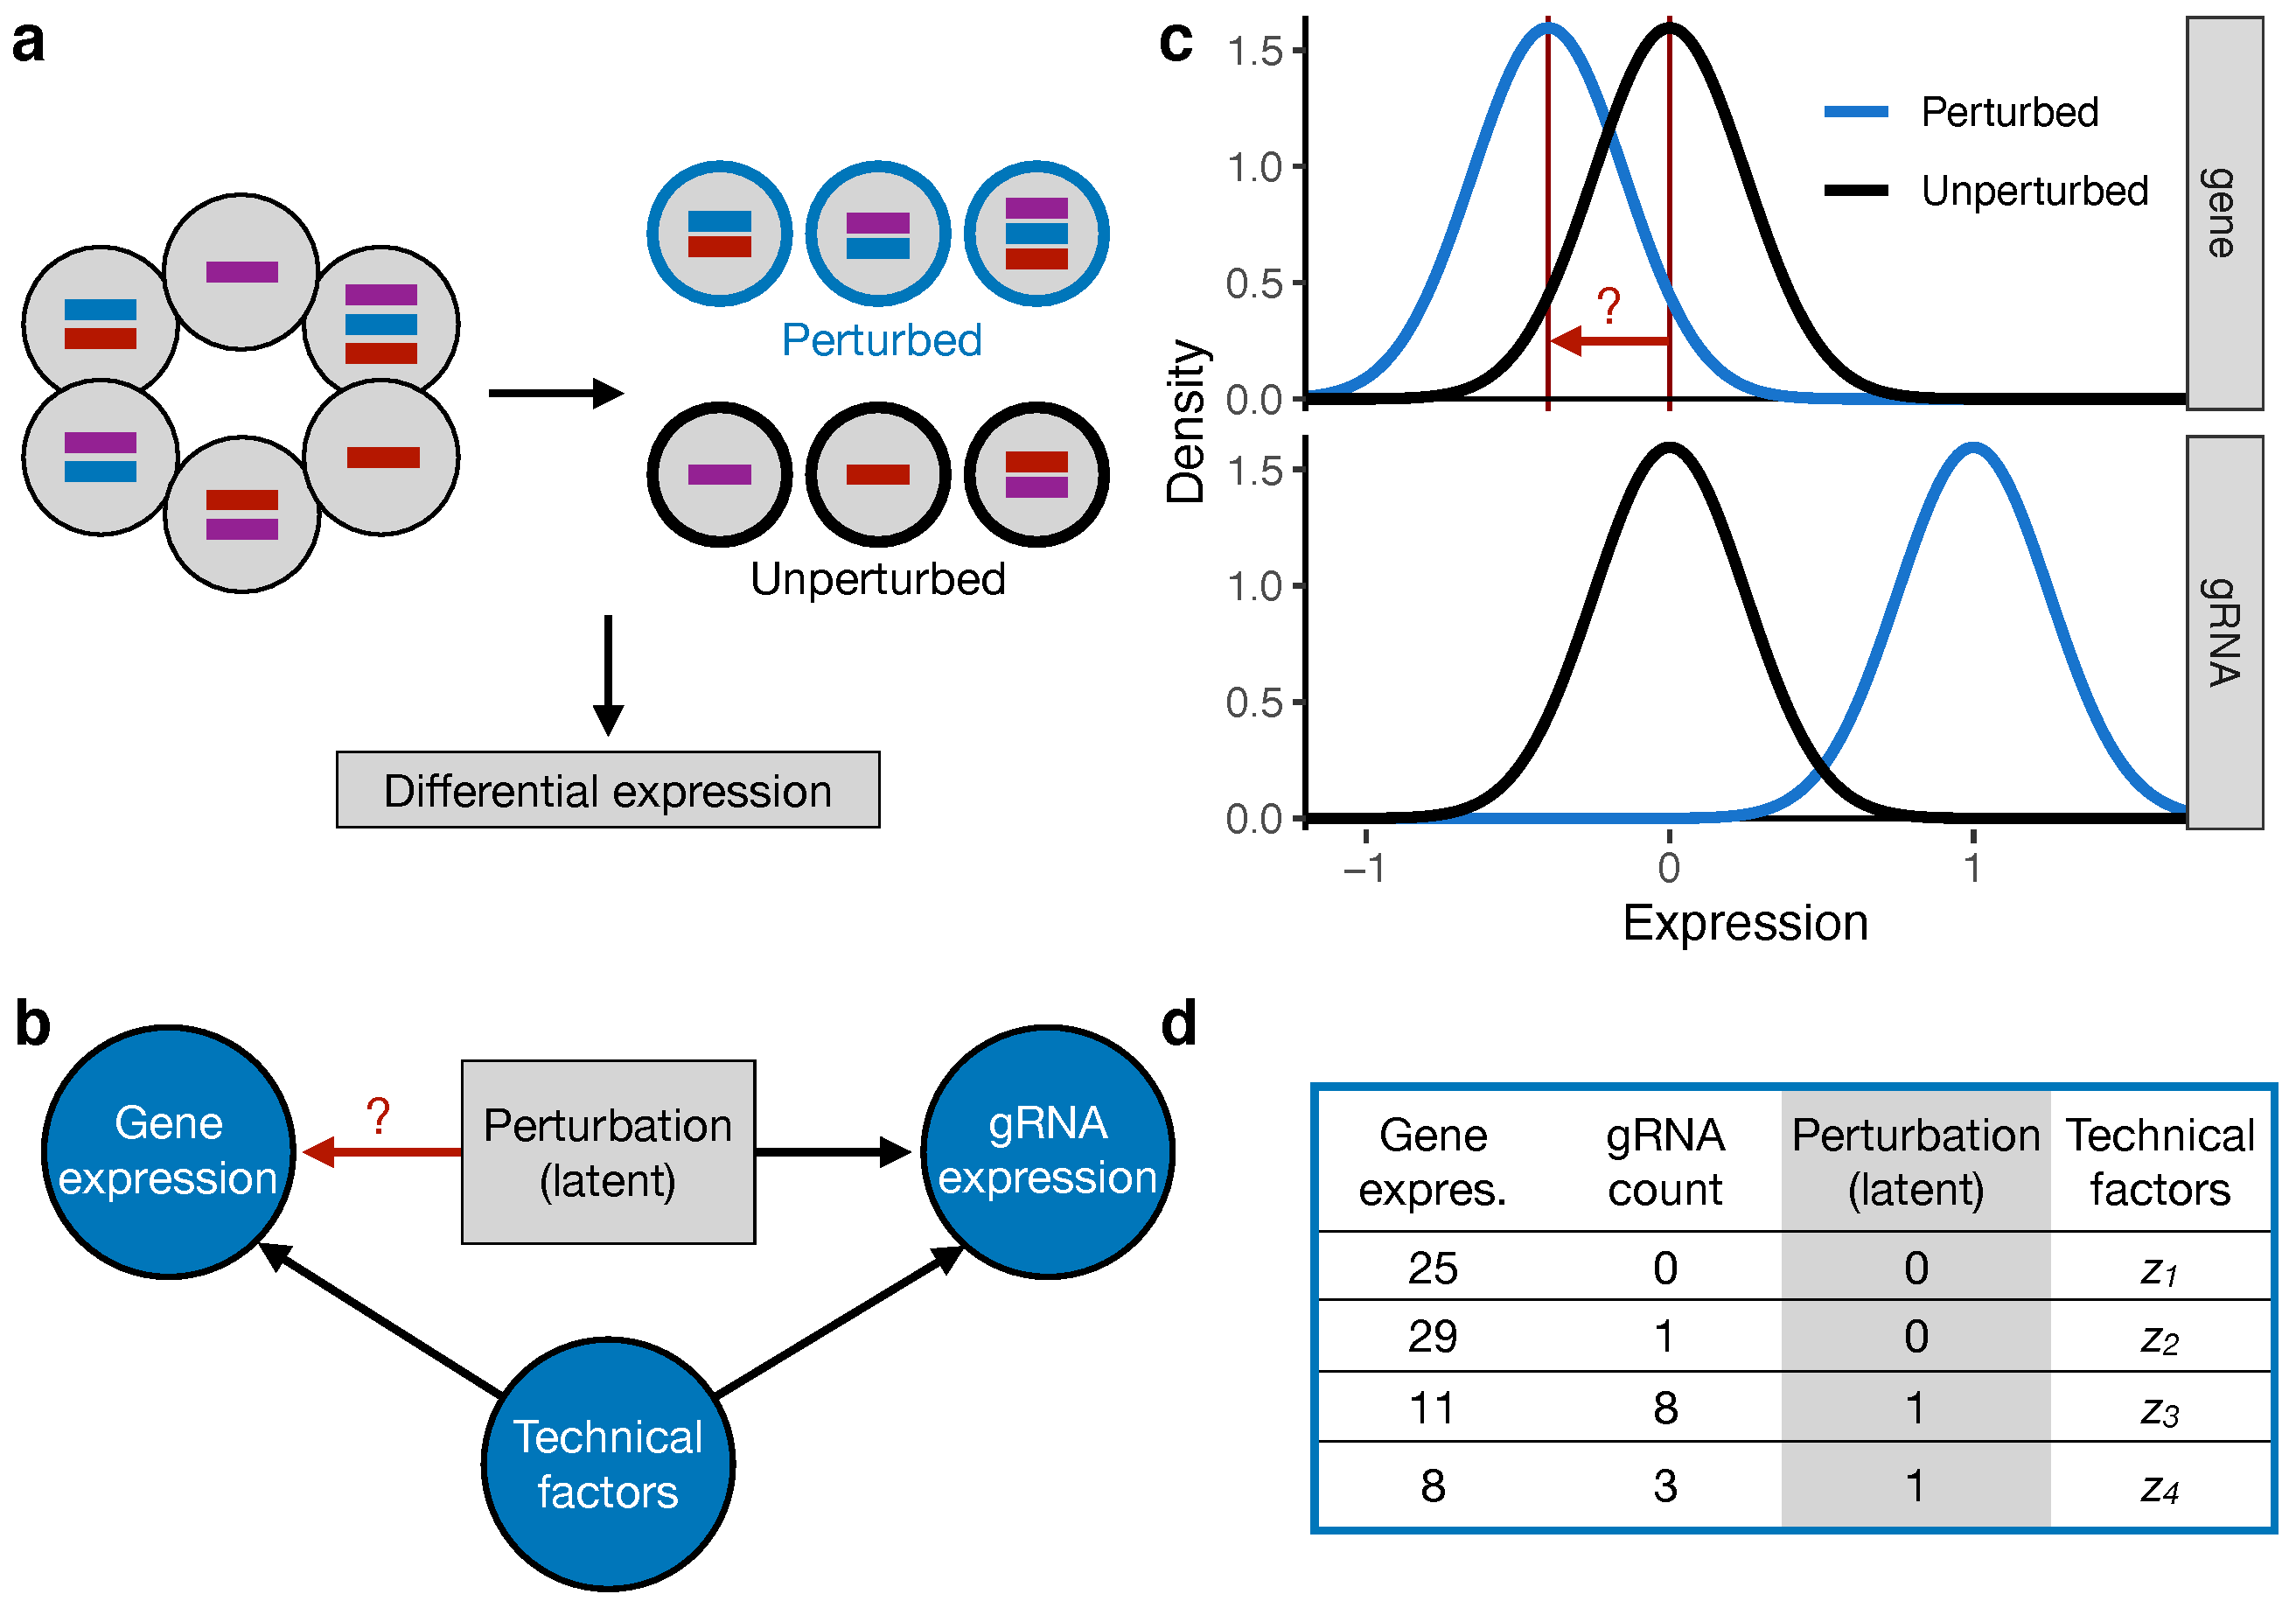
\includegraphics[width=1\linewidth]{../../figures/analysis_challenges/plot.pdf}
	\caption{\textbf{Experimental design and analysis challenges}: \textbf{a,} Experimental design. For a given perturbation (e.g., the perturbation indicated in blue), we partition the cells into two groups: perturbed and unperturbed. Next, for a given gene, we conduct a differential expression analysis across the two groups, yielding an estimate of the impact of the given perturbation on the given gene. \textbf{b,} DAG representing all variables in the system. The perturbation (latent) impacts both gene expression and gRNA expression; technical factors act as confounders, also impacting gene and gRNA expression. The target of estimation is the effect of the perturbation on gene expression. \textbf{c,} Schematic illustrating the ``background read'' phenomenon. Due to errors in the sequencing and alignment processes, unperturbed cells exhibit a nonzero gRNA count distribution (bottom). The target of estimation is the change in mean gene expression in response to the perturbation (top). \textbf{d}, Example data on four cells for a given perturbation-gene pair. Note that (i) the perturbation is unobserved, and (ii) the gene and gRNA data are discrete counts.}
	\label{analysis_challenges}
\end{figure}

\clearpage
% 2. Emprical challenges
\begin{figure}[h!]
	\centering
	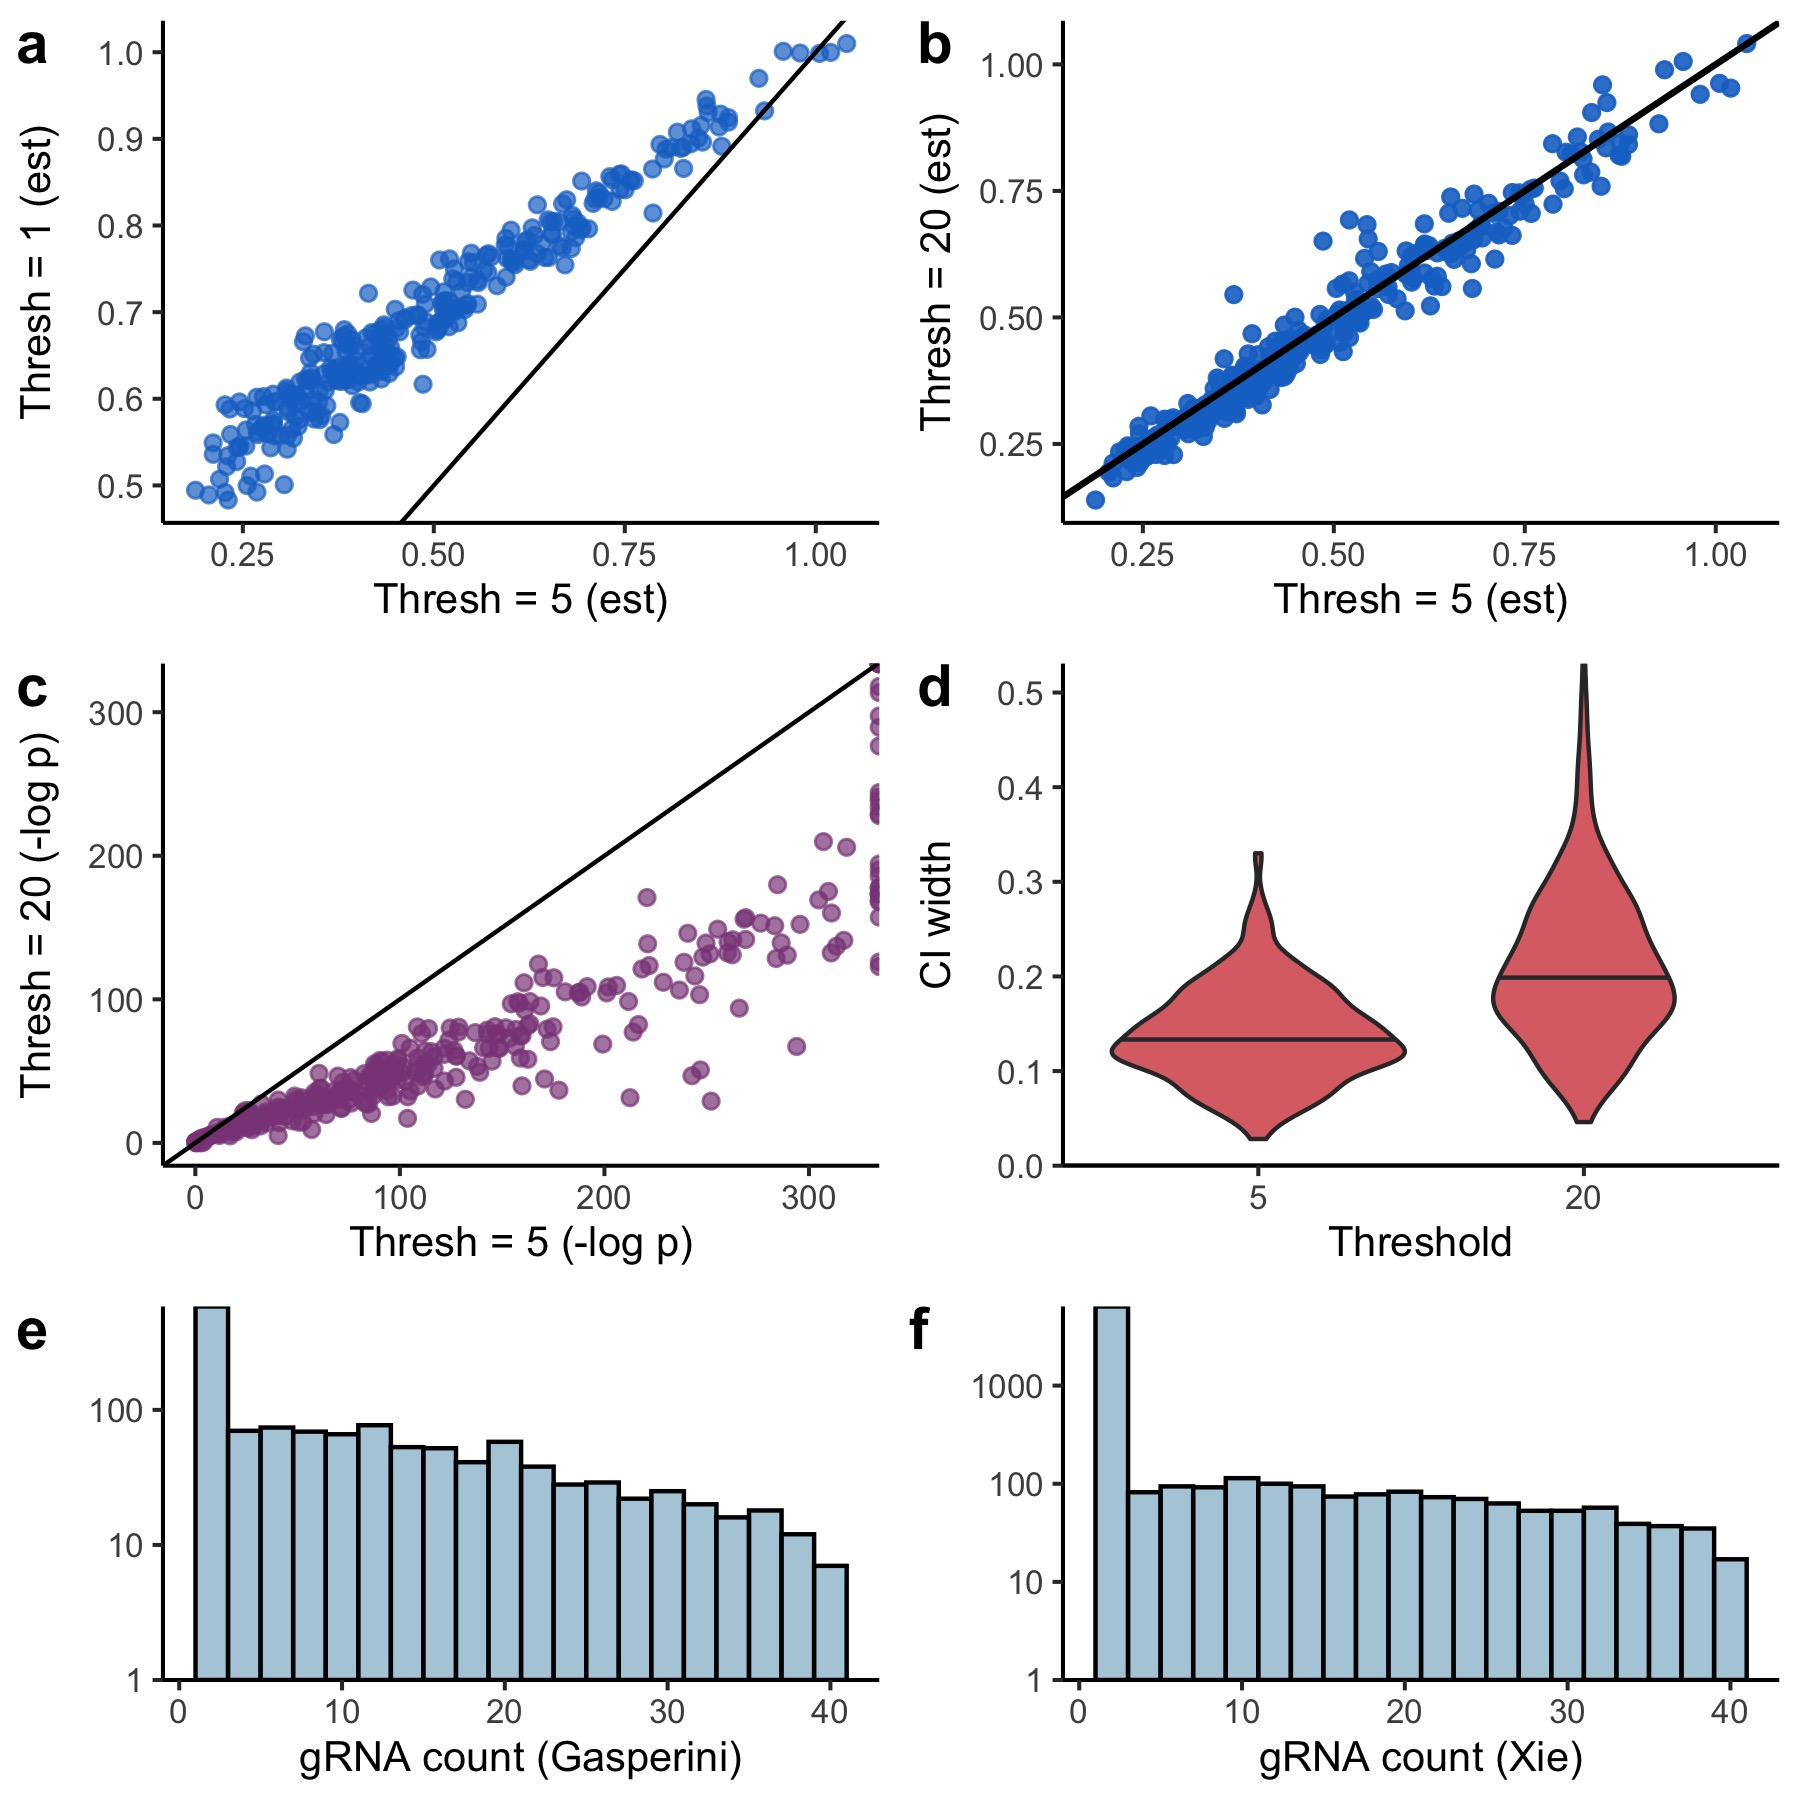
\includegraphics[width=1\linewidth]{../../figures/thresholding_empirical/plot}
	\caption{\textbf{Empirical challenges of thresholded regression.} \textbf{a-b,} Fold change estimates produced by threshold = 1 versus threshold = 5 (a) and threshold = 20 versus threshold = 5 (b). The selected threshold substantially impacts the results. \textbf{c-d,} $p$-values (c) and CI widths (d) produced by threshold = 20 versus threshold = 5. The latter threshold yields more confident estimates. \textbf{e-f}, Empirical distribution of randomly-selected gRNA from Gasperini (e) and Xie (f) data (0 counts not shown). The gRNA data do not appear to imply an obvious threshold selection strategy.}
	\label{thresholding_empirical}
\end{figure}

\clearpage
\begin{figure}[h!]
\centering
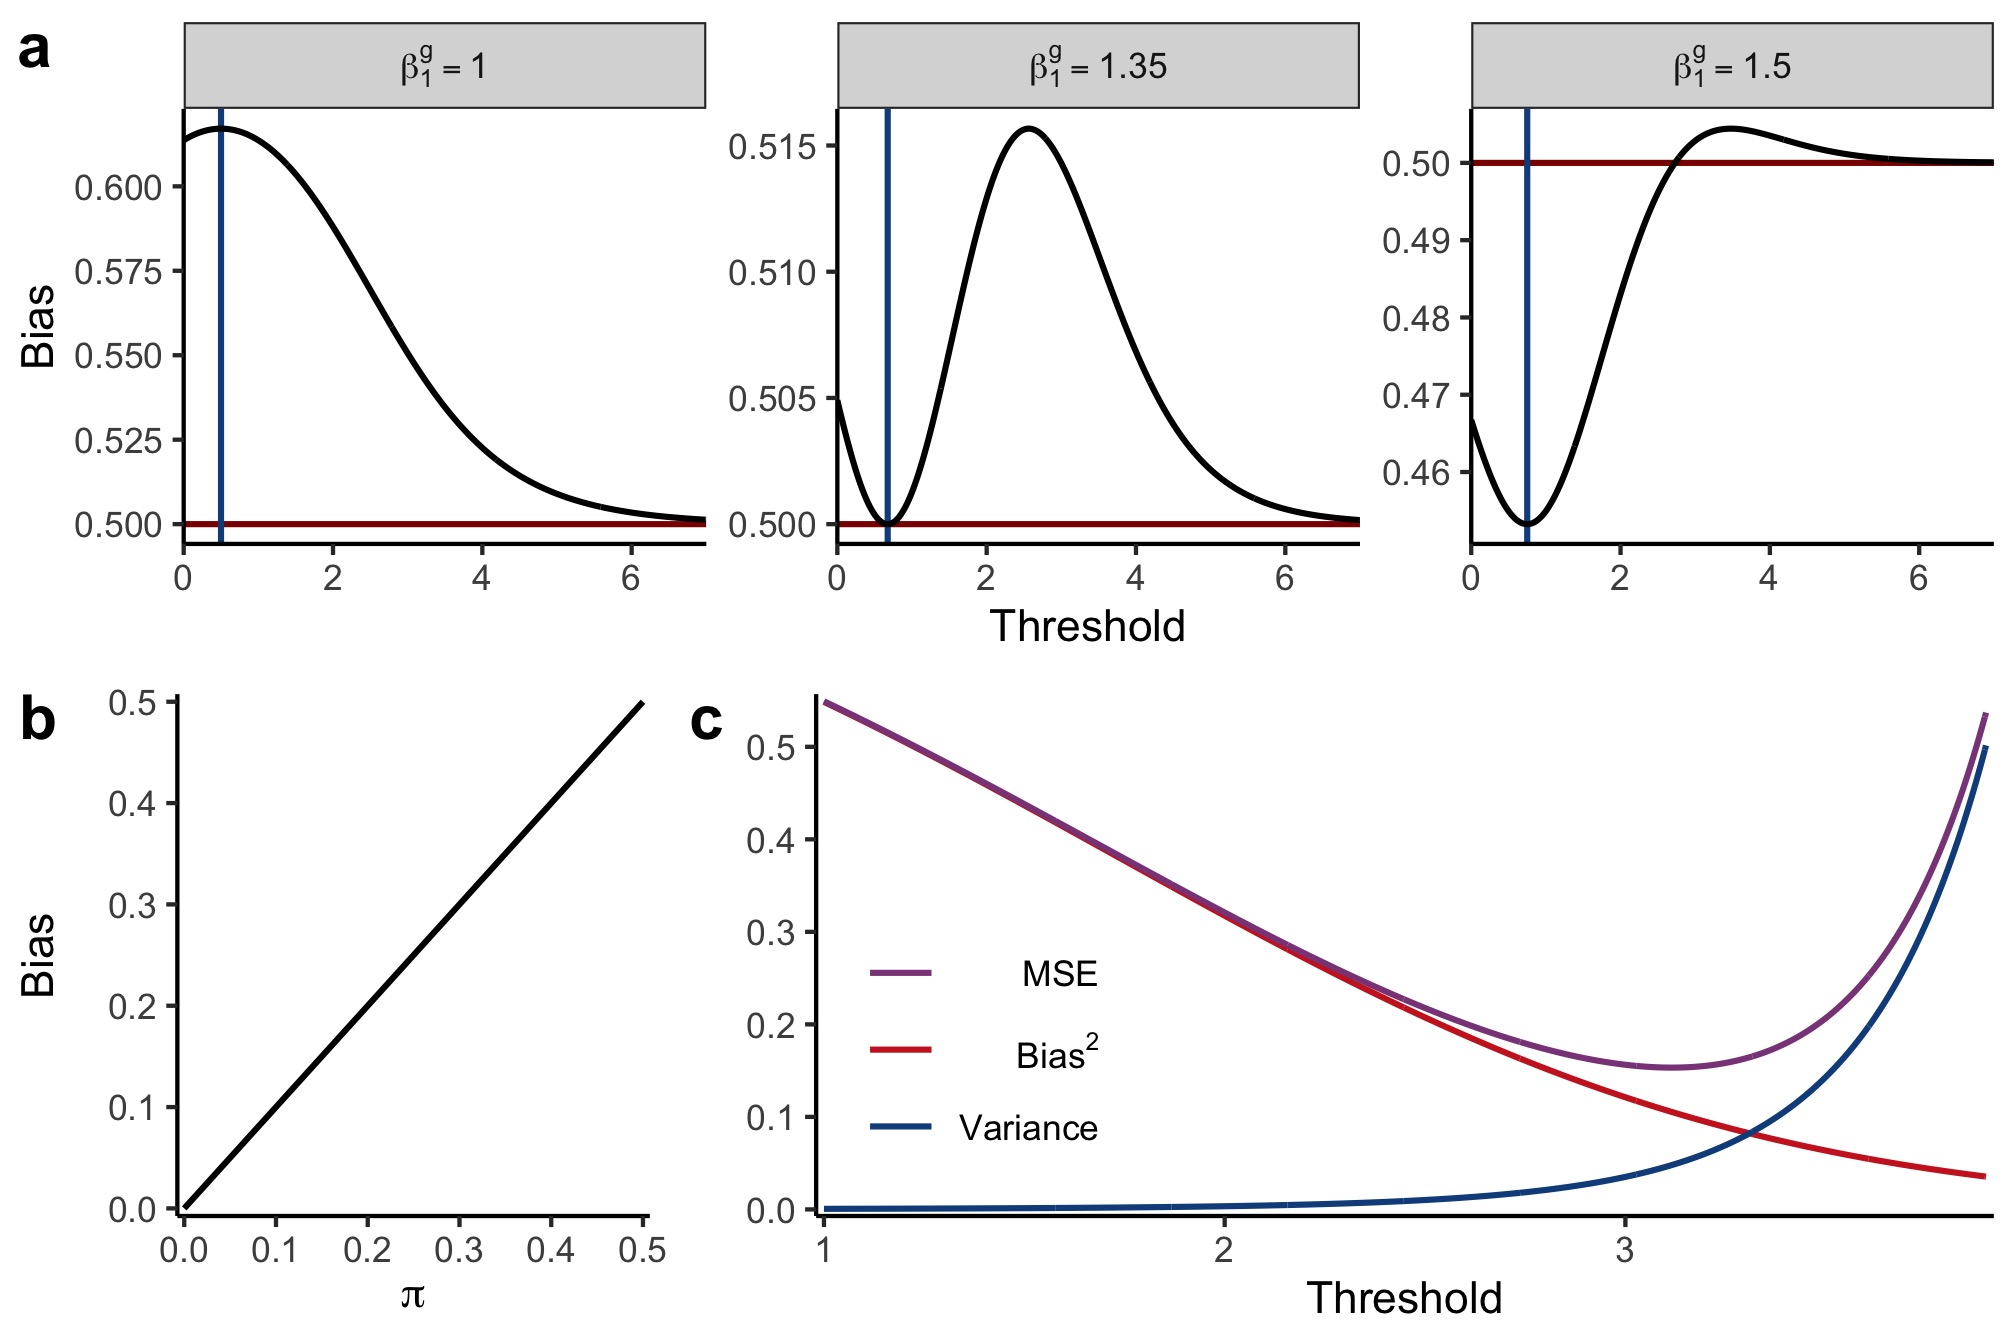
\includegraphics[width=0.7\linewidth]{../../figures/thresholding_theoretical/plot}
\caption{\textbf{Thresholding method bias-variance decomposition.} Bias decreases and variance increases as the threshold tends to infinity. $\beta^g_1 = 1, \beta^m_1 = 1,$ and $\pi = 0.1$ in this plot.}
\label{thresholding_theoretical}
\end{figure}


\clearpage
% Theory
\begin{figure}[h!]
	\centering
	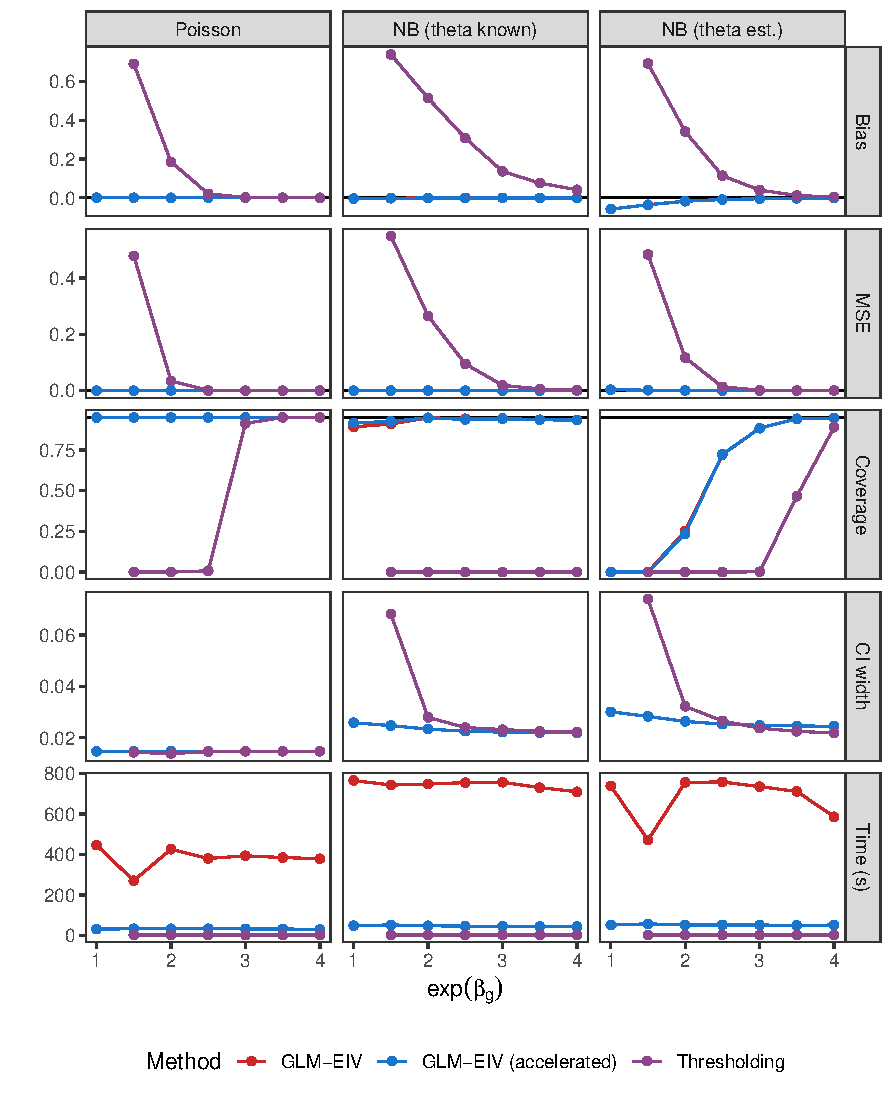
\includegraphics[width=0.9\linewidth]{../../figures/main_text_sim/plot}
	\caption{\textbf{Simulation study}. Columns correspond to distributions (Poisson, NB with known $\theta$, NB with estimated $\theta$), and rows correspond to metrics (bias, MSE, coverage, CI width, and time). Methods are shown in different colors; GLM-EIV (red) is masked by accelerated GLM-EIV (blue) in several panels. GLM-EIV demonstrated superior statistical performance to the thresholding method on all metrics (rows 1-4). Accelerated GLM-EIV had substantially lower computational cost than ``vanilla'' GLM-EIV (bottom row) despite demonstrating identical statistical performance (rows 1-4).}
	\label{main_text_sim}
\end{figure}

\clearpage
\begin{figure}
	\centering
	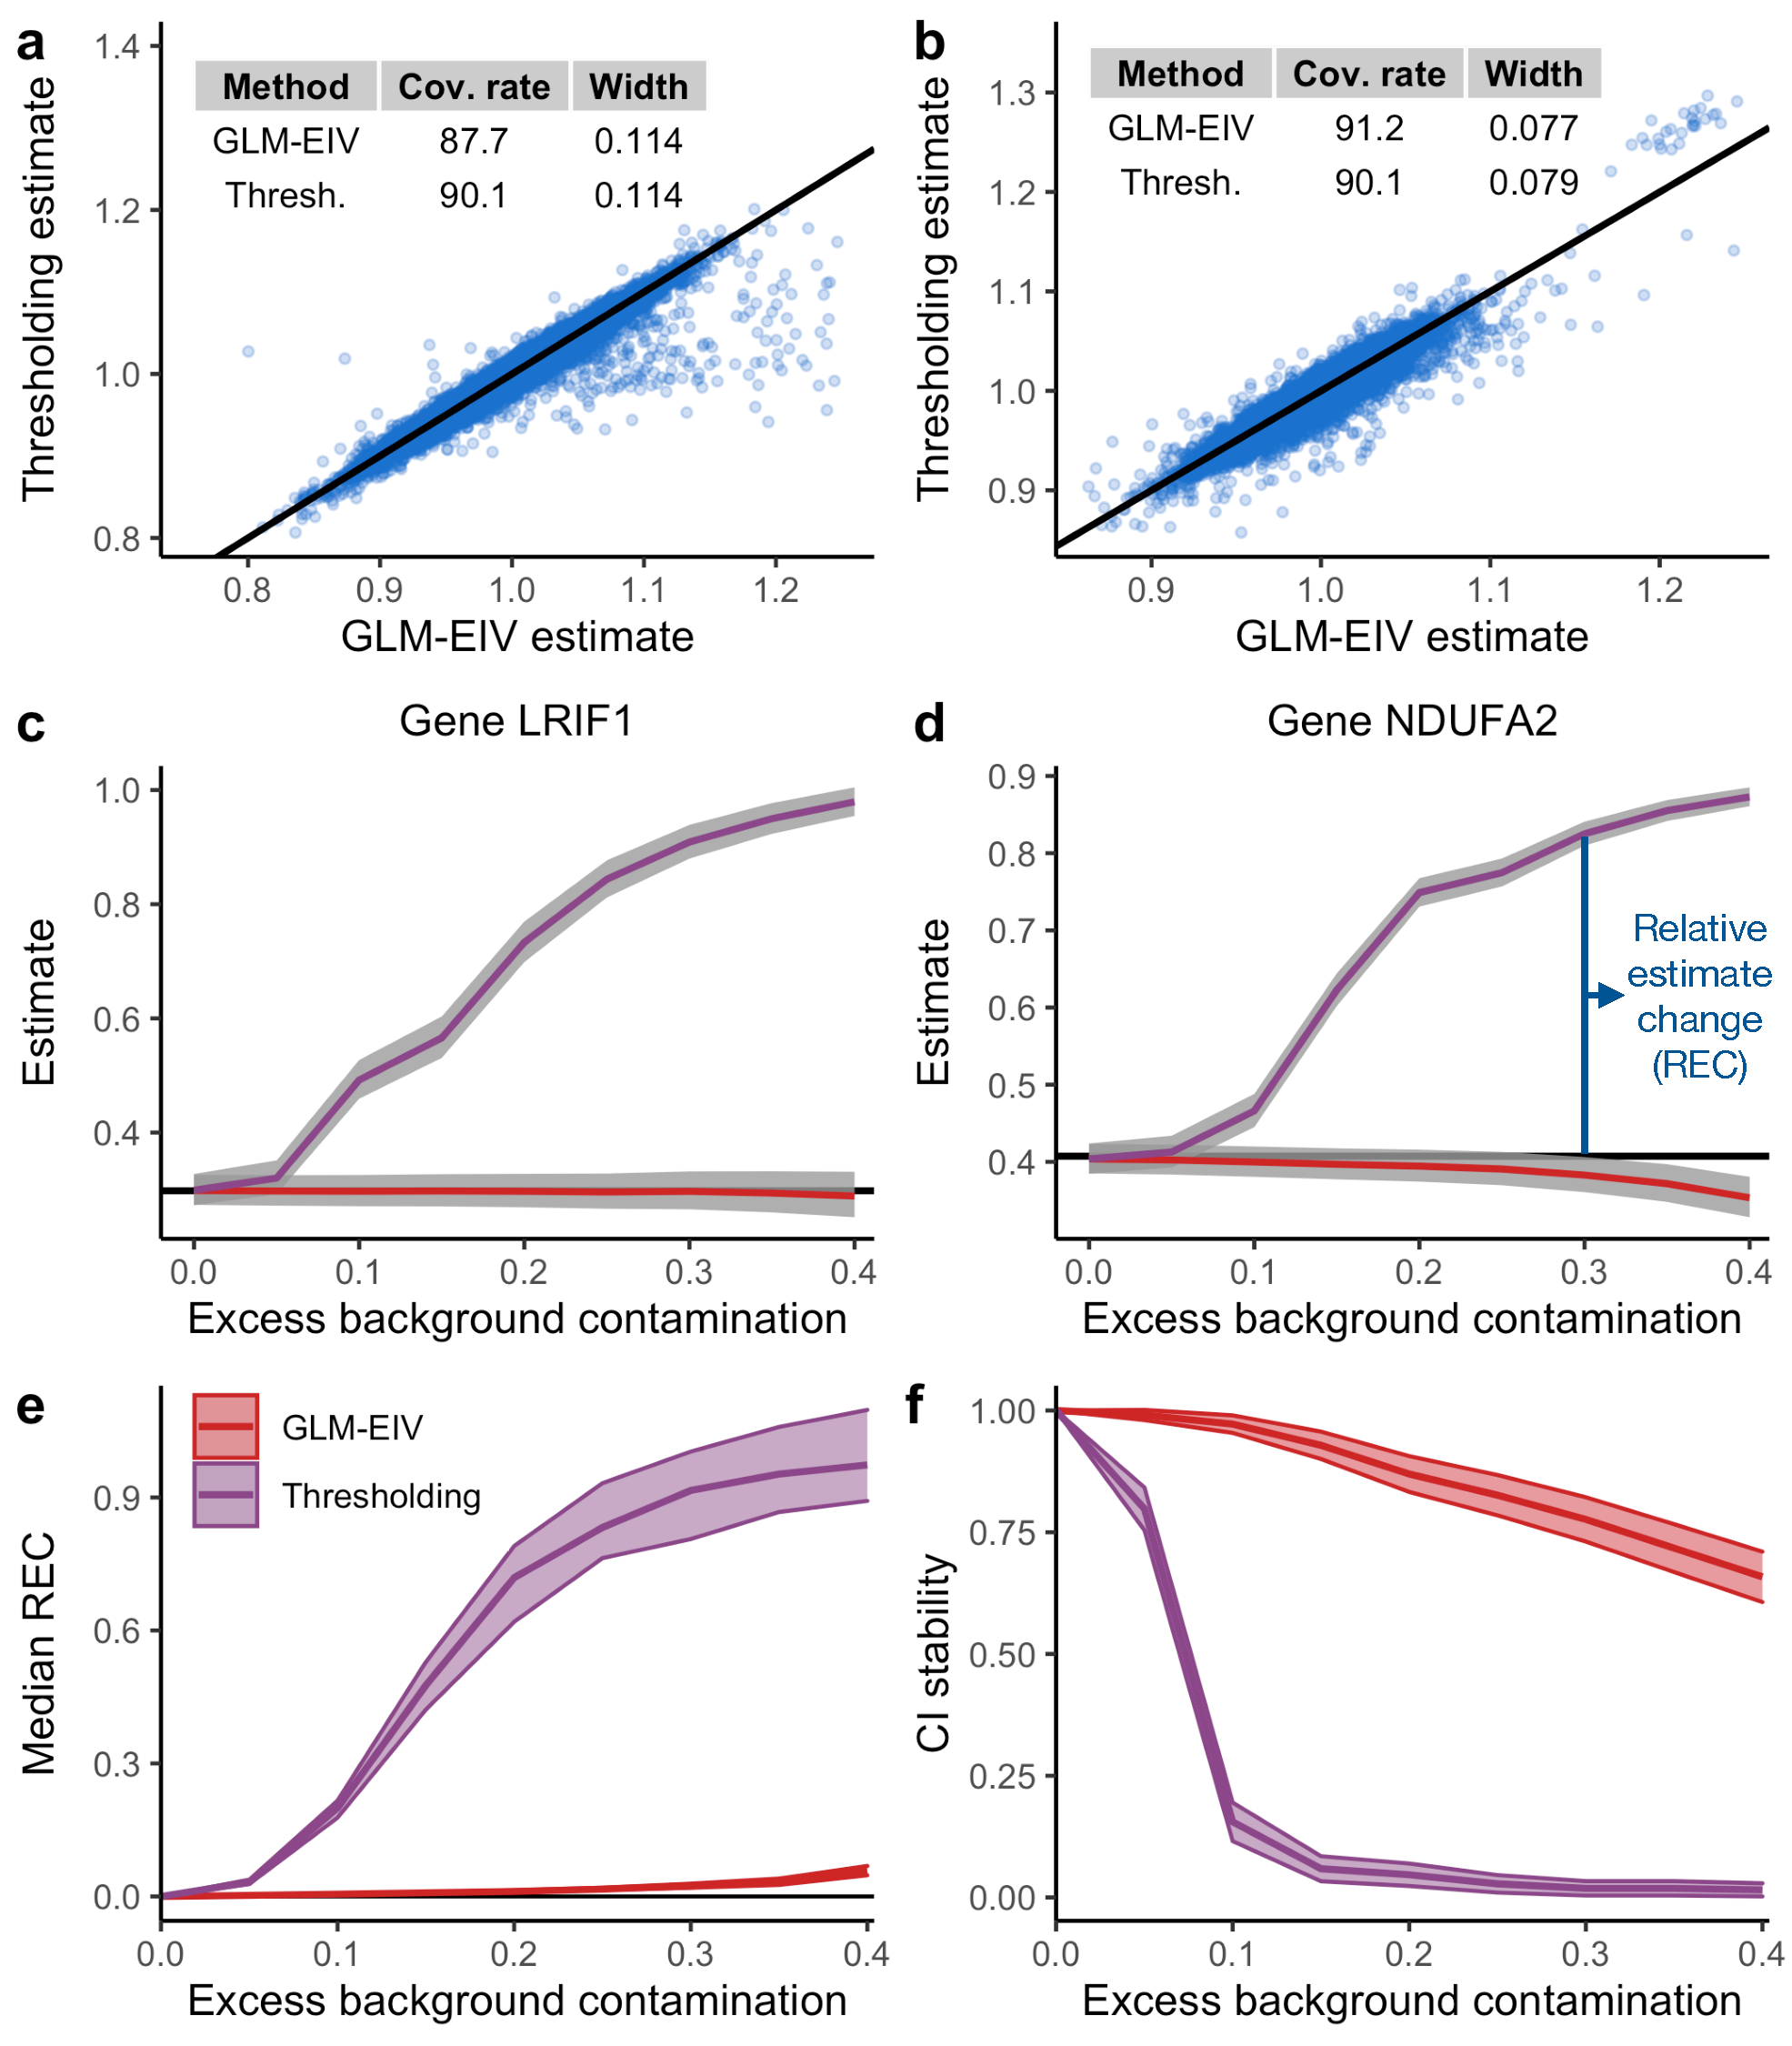
\includegraphics[width=0.9\linewidth]{../../figures/data_analysis/annotated_plot_crop}
	\caption{\textbf{Data analysis}. \textbf{a-b}, Estimates for fold change produced by GLM-EIV and thresholded regression on Gasperini (\textbf{a}) and Xie (\textbf{b}) negative control pairs. \textbf{c-d}, Estimates produced by GLM-EIV and thresholded regression on two positive control pairs -- \textit{LRIF1} (\textbf{a}) and \textit{NDUFA2} (\textbf{b}) -- plotted as a function of excess background contamination. Grey bands, 95\% CIs for the target of inference outputted by the methods. \textbf{e-f}, Median relative estimate change (REC; \textbf{e}) and confidence interval coverage rate (\textbf{f}) across \textit{all} 322 positive control pairs, plotted as a function of excess background contamination. Colored bands, pointwise 95\% CIs for population quantities. Panels (\textbf{c-f}) together illustrate that GLM-EIV demonstrated greater stability than thresholded regression as background contamination increased.}\label{fig:real_data}
\end{figure}

\clearpage
% Dec tree
\begin{figure}[h!]
	\centering
	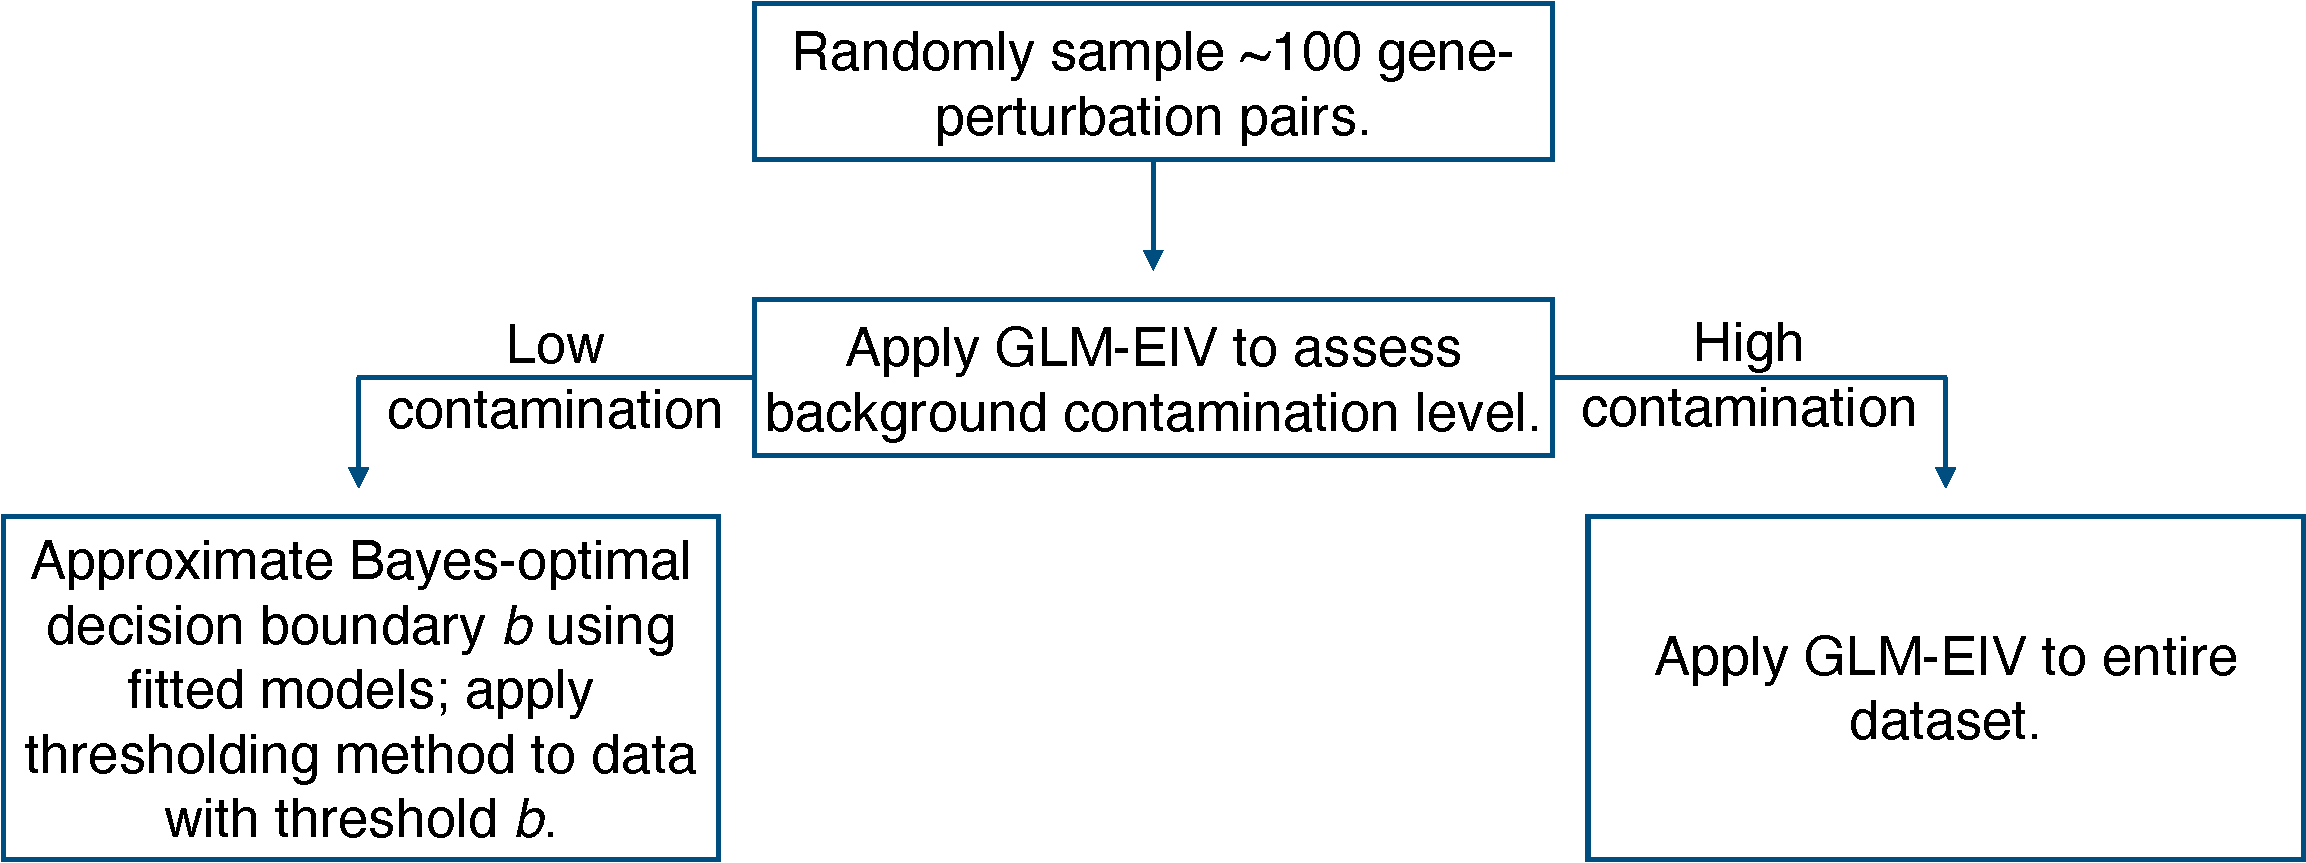
\includegraphics[width=0.9\linewidth]{../../figures/dec_tree/dec_tree_crop}
	\caption{\textbf{Use of GLM-EIV in practice}. The decision tree above illustrates how we anticipate GLM-EIV could be used in practice. First, apply GLM-EIV to a set of randomly-sampled gene-perturbation pairs to assess background contamination level (positive control pairs work best for this purpose). If GLM-EIV indicates that background contamination is high (e.g., $\exp(\beta^g_1) \lessapprox $ 10), apply GLM-EIV to analyze the entire dataset; otherwise, approximate the Bayes-optimal decision boundary using the fitted GLM-EIV models. Next, apply a thresholding method (e.g., SCEPTRE or thresholded negative binomial regression) to analyze the data, setting the threshold to the estimated Bayes-optimal decision boundary.}\label{fig:dec_tree}
\end{figure}
\clearpage
\begin{appendices}
\begin{refsection}
\section{Theoretical details for thresholding estimator}\label{sec:appendix_theory}

\subsection{Proposition statements}
This subsection contains detailed proposition statements for the informal claims made in Section \ref{sec:thresholding_theory}. For simplicity we derive results in the case $\pi = 1/2$. In reality $\pi$ is much closer to zero; however, setting $\pi$ to $1/2$ simplifies the proofs substantially and enables us to recover the most interesting and important statistical phenomena (e.g., attenuation bias, monotonic impact of $\beta^g_1$ on problem difficulty, etc.). We state state five propositions labeled \ref{prop:att_bias} -- \ref{prop:comparison} corresponding to the informal claims made in Section \ref{sec:thresholding_theory}; these propositions visually are depicted in Figure \ref{fig:bias_plot}.
 
First, the thresholding method incurs strict attenuation bias (i.e., it \textit{under}estimates the true effect size) for all choices of the threshold and over all possible values of the model parameters:
\begin{proposition}\label{prop:att_bias} Fix $\pi = 1/2$. For all $(\beta^g_1, c, \beta^g_0) \in \R^3$, the asymptotic relative bias is positive, i.e. 
	$$b(\beta^g_1, 1/2, c, \beta^g_0) > 0.$$
\end{proposition}

Next, the asymptotic relative bias $b$ decreases monotonically in $\beta^g_1:$
\begin{proposition}\label{prop:monotonic} Fix $\pi = 1/2$. The asymptotic relative bias $b$ decreases monotonically in $\beta_1^g$, i.e.
		$$\frac{\partial b}{\partial(\beta^g_1)}\left(\beta^g_1, 1/2, c, \beta^g_0\right) \leq 0.$$
\end{proposition}
Let $c_\textrm{bayes}$ denote the Bayes-optimal decision boundary for classifying cells as perturbed or unperturbed, i.e. $c_\textrm{bayes} = (1/2)(\beta^g_0 + \beta^g_1)$ for $\pi = 1/2$. We have that $c_\textrm{bayes}$ is a critical value of the bias function.
\begin{proposition}\label{prop:bayes_opt}
		For $\pi = 1/2$ and given $(\beta^g_1, \beta^g_0) \in \R^2$, the Bayes-optimal decision boundary $c_\textrm{bayes}$ is a critical value of the bias function $b$, i.e.
		$$ \frac{\partial b}{\partial c}\left(\beta^g_1, 1/2, c_\textrm{bayes}, \beta^g_0\right) = 0.$$
\end{proposition} Furthermore, as the threshold tends to infinity, the asymptotic relative bias $b$ tends to $\pi$.
\begin{proposition}\label{prop:c_limit}
	Assume without loss of generality that $\beta^g_1 > 0$. As the threshold $c$ tends to infinity, the asymptotic relative bias $b$ tends to $\pi,$ i.e.
	$$ \lim_{ c \to \infty } b(\beta^g_1, \pi, c, \beta^g_0) = \pi.$$
\end{proposition}
As a corollary, when $\pi = 1/2$, asymptotic relative bias tends to $1/2$ as $c$ tends to infinity. Finally, we compare two threshold selection strategies head-to-head: setting the threshold to an arbitrarily large number, and setting the threshold to the Bayes-optimal decision boundary.
\begin{proposition}\label{prop:comparison} Assume without loss of generality that $\beta^g_1 > 0$. For $\beta^g_1 \in [0, 2\Phi^{-1}(3/4))$, we have that $$b(\beta^g_1, 1/2, c_\textrm{bayes}, \beta^g_0) > b(\beta^g_1, 1/2, \infty, \beta^g_0).$$ For $\beta^g_1 = 2\Phi^{-1}(3/4)$, we have that $$b(\beta^g_1, 1/2, c_\textrm{bayes}, \beta^g_0) = b(\beta^g_1, 1/2, \infty, \beta^g_0).$$ Finally, for $\beta^g_1 \in (2\Phi^{-1}(3/4), \infty)$, we have that $$b(\beta^g_1, 1/2, c_\textrm{bayes}, \beta^g_0) < b(\beta^g_1, 1/2, \infty, \beta^g_0).$$
\end{proposition}
In other words, setting the threshold to a large number yields a smaller bias when $\beta^g_1$ is small (i.e., $\beta^g_1 < 2\Phi^{-1}(3/4) \approx 1.35$; Figure \ref{thresholding_theoretical}a, left); setting the threshold to the Bayes-optimal decision boundary yields a smaller bias when $\beta^g_1$ is large (i.e., $\beta^g_1 > 2\Phi^{-1}(3/4)$; Figure \ref{thresholding_theoretical}a, right); and the two approaches coincide when $\beta^g_1$ is intermediate (i.e., $\beta^g_1 = 2\Phi^{-1}(3/4)$; Figure \ref{thresholding_theoretical}a, middle).

\begin{figure}[h!]
	\centering
	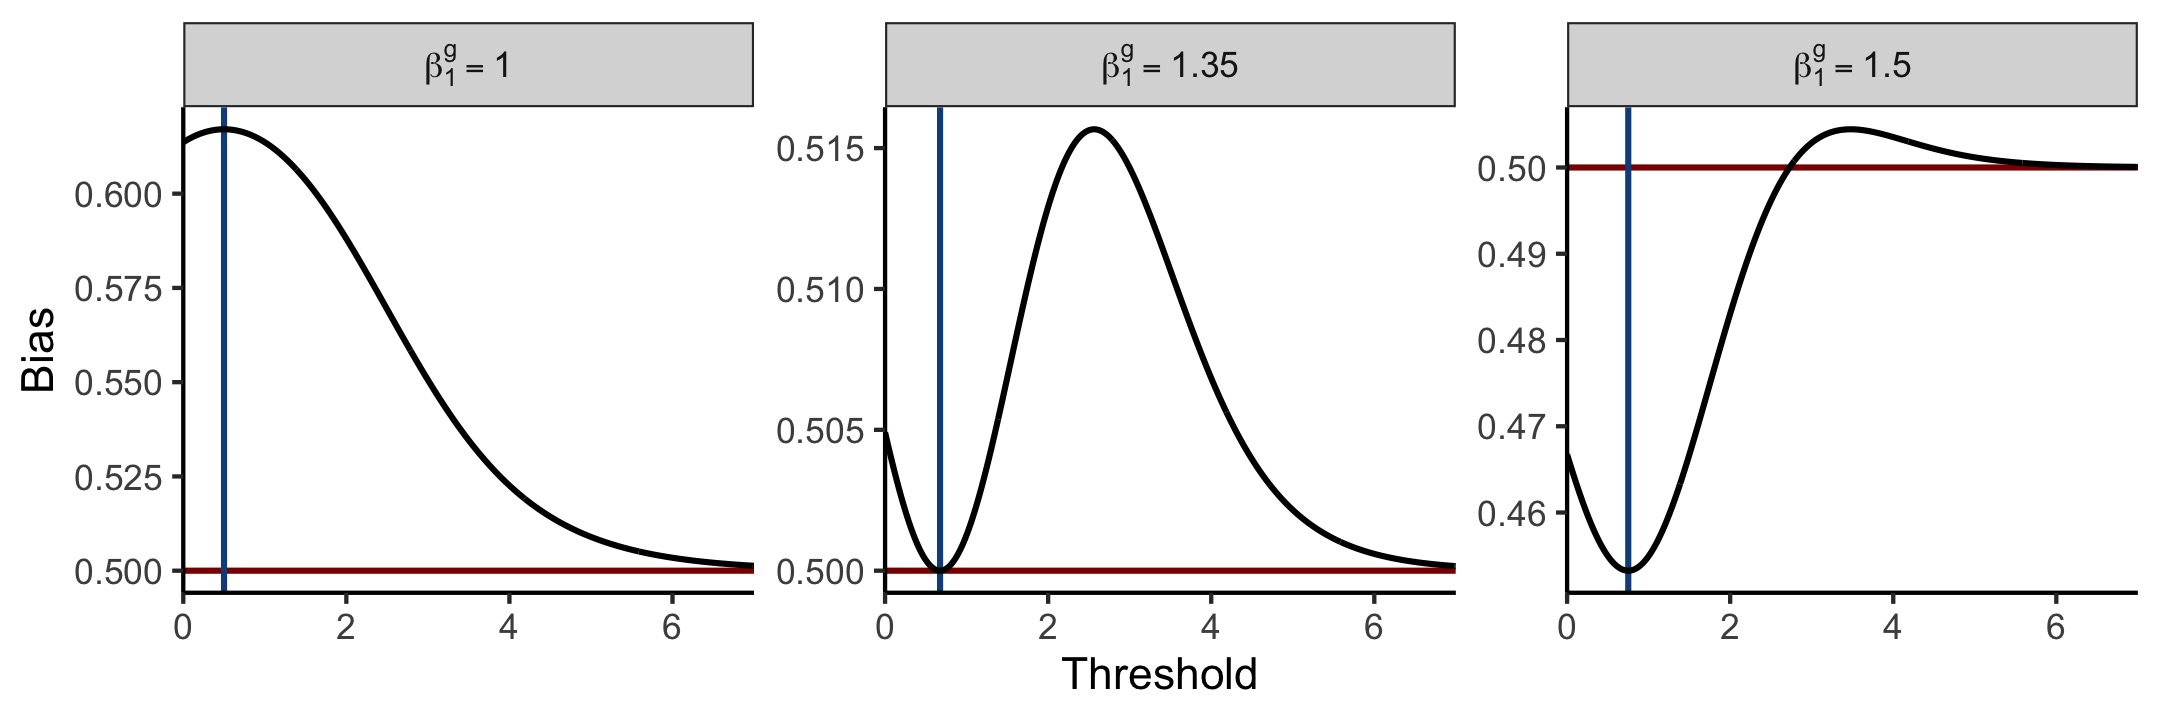
\includegraphics[width=1\linewidth]{../../figures/thresholding_theoretical/app_plot}
	\caption{\textbf{Bias as a function of threshold}. This figure visually depicts Propositions \ref{prop:att_bias}-\ref{prop:comparison}, which were stated informally in the main text. Asymptotic relative bias is plotted on the vertical axis, and the threshold is plotted on the horizontal axis. Panels correspond to different values of $\beta^g_1$. Vertical blue lines indicate the Bayes-optimal decision boundary. Observe that (a) bias is strictly nonzero (proposition \ref{prop:att_bias}); (b) bias decreases monotonically in $\beta^g_1$ (Proposition \ref{prop:monotonic}); (c) the Bayes-optimal decision boundary is a critical value of the bias function (Proposition \ref{prop:bayes_opt}), in some cases a maximum and in other cases a minumum; (d) as the threshold tends to infinity, the bias converges to $1/2$ (Proposition \ref{prop:c_limit}).; and (e) when $\beta^g_1 < 1.35$, an arbitrarily large number yields a smaller bias; by contrast, when $\beta^g_1 > 1.35$, the Bayes-optimal decision boundary yields a smaller bias (Proposition \ref{prop:comparison}).
	%Across all panels, $\beta^g_0 = 0$ and $\pi = 1/2$. When $\beta^g_1$ is small, setting the threshold to an arbitrarily large number yields a smaller bias than setting the threshold to the Bayes-optimal decision boundary; when $\beta^g_1$ is large, the opposite is true.
}
	\label{fig:bias_plot}
\end{figure}


\subsection{Organization} The following subsections prove all propositions. Section (\ref{sec:notation}) introduces some notation. Section (\ref{sec:convergence}) establishes almost sure convergence of the thresholding estimator in the model (\ref{theoretical_model}), proving Proposition \ref{prop:convergence}. Section (\ref{sec:simplication}) simplifies the expression for the attenuation function $\gamma$, and section (\ref{sec:derivatives})  computes derivatives of $\gamma$ to be used throughout the proofs. Section (\ref{sec:c_limit}) establishes the limit in $c$ of $\gamma$, proving Proposition \ref{prop:c_limit}. Section (\ref{sec:bayes_opt}) establishes that the Bayes-optimal decision boundary is a critical value of $\gamma$, proving Proposition \ref{prop:bayes_opt}, and section (\ref{sec:comparison}) compares the competing threshold selection strategies head-to-head, proving Proposition \ref{prop:comparison}. Section (\ref{sec:monotone}) demonstrates that $\gamma$ is monotone in $\beta^g_1$, proving Proposition \ref{prop:monotonic}, and Section (\ref{sec:att_bias}) establishes attenuation bias of the thresholding estimator, proving Proposition \ref{prop:att_bias}. Finally, Section (\ref{sec:bv_decomp}) derives the bias-variance decomposition of the thresholding estimator in the no-intercept version of (\ref{theoretical_model}), proving Proposition \ref{prop:bv_decomp}.

% Labels of propositions and theorems
% propositions:
% prop:convergence
% prop:att_bias
% prop:bayes_opt
% prop:c_limit_half
% prop:comparison
% prop:monotonic
% prop:c_limit
% prop:bv_decomp

% sections
% sec:notation
% sec:convergence
% sec:simplication
% sec:derivatives
% sec:c_limit
% sec:bayes_opt
% sec:comparison
% sec:beta_lim
% sec:monotone
% sec:att_bias
% sec:bv_decomp
\subsection{Notation}\label{sec:notation}
 All notation introduced in this subsection (i.e., \ref{sec:notation}) pertains to the Gaussian model with intercepts (\ref{theoretical_model}). Recall that the attenuation function $\gamma: \R^4 \to \R$ is defined by
$$ \gamma(\beta^g_1, c, \pi, \beta^g_0) = \frac{\pi(\omega - \E[\hat{p}_i])}{ \E[\hat{p}_i](1 -\E[\hat{p}_i])},$$ where $$\E[\hat{p}_i] = \zeta(1-\pi) + \omega\pi; \quad \omega = \Phi\left(\beta_1^g + \beta_0^g - c \right); \quad \zeta = \Phi\left( \beta^g_0 - c \right).$$ Additionally, recall that the asymptotic relative bias function $b: \R^4 \to \R$ is
$$ b(\beta^g_1, c, \pi, \beta^g_0) = 1 - \gamma(\beta^g_1, c, \pi, \beta^g_0).$$ Next, we define the functions $g$ and $h: \R^4 \to \R$ by
\begin{equation}\label{def_g}
g(\beta^g_1, c, \pi, \beta^g_0) = (1-\pi)\left( \Phi(\beta_0^g + \beta_1^g - c)\right) - (1-\pi)\left(\Phi(\beta_0^g - c)\right)\end{equation}
 and
\begin{multline}\label{def_h}
h(\beta^g_1, c, \pi, \beta^g_0) = \left[(1-\pi)\left( \Phi(\beta_0^g - c)\right) + \pi\left(\Phi(\beta^g_0 + \beta^g_1 - c) \right) \right] \cdot \\ \left[(1-\pi)\left( \Phi(c - \beta^g_0) \right) + \pi\left(\Phi(c - \beta_0^g - \beta_1^g) \right) \right].
\end{multline}
We use $f:\R \to \R$ to denote the $N(0,1)$ density, and we denote the right-tail probability probability of $f$ by $\bar{\Phi}$, i.e.,
$$\bar{\Phi}(x) = \int_{x}^{\infty} f = \Phi(-x).$$

The parameter $\beta^g_0$ is a given, fixed constant throughout the proofs. Therefore, to minimize notation, we typically use $\gamma(\beta^g_1, c, \pi)$ (resp., $b(\beta^g_1, c, \pi),$ $g(\beta^g_1, c, \pi),$ $h(\beta^g_1, c, \pi)$) to refer to the function $\gamma$ (resp., $b, g, h$) evaluated at $(\beta^g_1, c, \pi, \beta^g_0)$. Finally, for a given function $r: \R^{p} \to \R$, point $x \in \R^p$, and index $i \in \{1, \dots, p\}$, we use the symbol $D_i r(x)$ to refer to the derivative of the $i$th component of $r$ evaluated at $x$ (\textit{sensu} \cite{fitzpatrick2009}). For example, $D_1 \gamma(\beta^g_1, c, 1/2)$ is the derivative of the first component of $\gamma$ (the component corresponding to $\beta^g_1$) evaluated at $(\beta^g_1, c, 1/2)$. Likewise,  $D_2g(\beta^g_1, c, \pi)$ is the derivative of the second component of $g$ (the component corresponding to $c$) evaluated at $(\beta^g_1, c, \pi).$

\subsection{Almost sure limit of $\hat{\beta}^m_1$}\label{sec:convergence}

We derive the limit in probability of $\hat{\beta}^m_1$ for the Gaussian model with intercepts (\ref{theoretical_model}). Dividing by $n$ in (\ref{thresh_est_intercepts}), we can express $\hat{\beta}^m_1$ as
$$ \hat{\beta}^m_1 = \frac{ \frac{1}{n} \sum_{i=1}^n ( \hat{p}_i - \overline{\hat{p}_i})(m_i - \overline{m})}{ \frac{1}{n} \sum_{i=1}^n (\hat{p}_i - \overline{\hat{p}})}.$$ By weak LLN,
$$ \hat{\beta}^m_1 \xrightarrow{P} \frac{\textrm{Cov}(\hat{p}_i, m_i)}{\V\left(\hat{p}_i\right)}.$$ To compute this quantity, we first compute several simpler quantities:
\begin{itemize}
\item[1.] Expectation of $m_i$: $\E[m_i] = \beta^m_0 + \beta^m_1\pi.$
\item[2.] Expectation of $\hat{p}_i$: \begin{multline*}
\E[\hat{p}_i] = \P\left[\hat{p}_i = 1\right] = \P\left[\beta^g_0 + \beta^g_1 p_i + \tau_i \geq c \right] = \\ \textrm{(By LOTP) } \P\left[ \beta^g_0 + \tau_i \geq c \right]\P\left[p_i = 0\right] + \P\left[ \beta^g_0 + \beta^g_1 + \tau_i \geq c \right] \P[p_i = 1] \\ = \P\left[ \tau_i \geq c - \beta^g_0\right](1- \pi) + \P\left[ \tau_i \geq c - \beta^g_1 - \beta^g_0 \right](\pi) \\ =  \left(\bar{\Phi}(c - \beta^g_0) \right) (1 - \pi) + \left( \bar{\Phi}(c - \beta^g_1 - \beta^g_0) \right)(\pi) = \\  \Phi(\beta^g_0 - c) (1-\pi) + \Phi(\beta^g_1 + \beta^g_0 - c) \pi = \zeta(1-\pi) + \omega \pi.
\end{multline*}
\item[3.] Expectation of $\hat{p}_i p_i$: 
$\E\left[ \hat{p}_i p_i \right] = \E\left[\hat{p}_i | p_i = 1 \right] \P\left[ p_i =1 \right] = \P\left[ \beta^g_0 + \beta^g_1 + \tau_i \geq c \right] \pi = \omega \pi.$
\item[4.] Expectation of $\hat{p}_i m_i$:
\begin{multline*}
\E\left[\hat{p}_i m_i\right] = \E[\hat{p}_i (\beta^m_0 + \beta^m_1 p_i + \ep_i)] = \beta^m_0 \E\left[\hat{p}_i\right] + \beta^m_1 \E\left[\hat{p}_i p_i\right] + \E[\hat{p}_i \ep_i] \\ = \beta^m_0 \E[\hat{p}_i] + \beta^m_1 \omega \pi + \E[\hat{p}_i] \E[\ep_i] = \beta^m_0 \E[\hat{p}_i] + \beta^m_1 \omega \pi.
\end{multline*}
\item[5.] Variance of $\hat{p}_i$: Because $\hat{p}_i$ is binary, we have that $\V[\hat{p}_i] = \E[\hat{p}_i]\left(1 - \E[\hat{p}_i]\right) .$
\item[6.] Covariance of $\hat{p}_i, m_i$:
\begin{multline*}
\textrm{Cov}\left(\hat{p}_i, m_i\right) = \E\left[\hat{p}_i m_i\right] - \E[\hat{p}_i] \E[m_i] = \beta^m_0 \E[\hat{p}_i] + \beta^m_1 \omega \pi - \E[\hat{p}_i]( \beta^m_0 + \beta^m_1 \pi)\\ = \beta^m_1 \omega \pi - \E[\hat{p}_i] \beta_1^m \pi = \beta^m_1 \pi \left( \omega - \E[\hat{p}_i]\right).
\end{multline*}
Combining these expressions, we have that
$$ \hat{\beta}^m_1 \xrightarrow{P} \frac{\beta^m_1 \pi (\omega - \E[\hat{p}_i])}{\E[\hat{p}_i](1 - \E[\hat{p}_i])} = \beta^m_1 \gamma(\beta^g_1, c, \pi).$$
\end{itemize}

\subsection{Re-expressing $\gamma$ in a simpler form}\label{sec:simplication}
We rewrite the attenuation fraction $\gamma$ in a way that makes it more amenable to theoretical analysis. We leverage the fact that $f$ integrates to unity and is even. We have that
\begin{equation}\label{thm:gamma_expression_1} \E\left[\hat{p}_i\right] = (1 - \pi) \bar{\Phi}(c - \beta_0^g) + \pi \bar{\Phi}(c - \beta^g_0 - \beta^g_1) = (1 - \pi) \Phi(\beta_0^g - c) + \pi\Phi(\beta^g_0 + \beta^g_1 - c), \end{equation}
 and so \begin{multline}\label{thm:gamma_expression_2} 1 - \E\left[\hat{p}_i\right] = (1 - \pi) + \pi - \E[\hat{p}_i]  = (1-\pi) \left(1 - \bar{\Phi}(c - \beta_0^g)\right)  + \pi \left(1 - \bar{\Phi}(c - \beta^g_0 - \beta^g_1) \right) \\ = (1 - \pi)\Phi(c - \beta^g_0) + \pi \Phi(c - \beta_0^g - \beta_1^g).
\end{multline}
Next,
\begin{equation}\label{thm:gamma_expression_3}
\omega = \Phi(\beta^g_1 + \beta^g_0 - c),\end{equation} and so
\begin{multline}\label{thm:gamma_expression_4}
\omega - \E[\hat{p}_i] = \Phi(\beta^g_1 + \beta^g_0 - c) - (1-\pi)\Phi(\beta^g_0 - c) - \pi \Phi(\beta^g_0 + \beta^g_1 - c)  \\ (1-\pi)\Phi(\beta^g_1 + \beta^g_0 - c)  - (1-\pi)\Phi(\beta^g_0 - c).
\end{multline}
Combining (\ref{thm:gamma_expression_1}, \ref{thm:gamma_expression_2}, \ref{thm:gamma_expression_3}, \ref{thm:gamma_expression_4}), we find that
\begin{multline}\label{gamma_alternative}
\gamma(\beta^g_1, c, \pi) = \frac{\pi(\omega - \E[\hat{p}_i])}{\E[\hat{p}_i](1 - \E[\hat{p}_i])} \\ = \frac{\pi \left[(1 - \pi) \Phi(\beta_0^g + \beta_1^g - c) - (1 - \pi) \Phi(\beta_0^g - c)\right]}{\left[(1-\pi)\Phi(\beta_0^g - c) + \pi \Phi(\beta^g_0 + \beta^g_1 - c) \right] \left[(1 - \pi) \Phi(c - \beta^g_0) + \pi\Phi(c - \beta_0^g - \beta_1^g) \right]}.
\end{multline}
As a corollary, when $\pi = 1/2$,
\begin{equation}\label{gamma_alternative_pi_half}
\gamma(\beta^g_1, c, 1/2)  \\ = \frac{\Phi(\beta_0^g + \beta_1^g - c) - \Phi(\beta_0^g - c) }{\left[\Phi(\beta_0^g - c) +\Phi(\beta^g_0 + \beta^g_1 - c)\right] \left[\Phi(c - \beta^g_0) + \Phi(c - \beta_0^g - \beta_1^g) \right]}.
\end{equation}
Recalling the definitions of $g$ (\ref{def_g}) and $h$ (\ref{def_h}), we can write $\gamma$ as
$$ \gamma(\beta^g_1, c, \pi) = \frac{\pi g(\beta^g_1, c, \pi)}{h(\beta^g_1, c,\pi)}.$$
The special case (\ref{gamma_alternative_pi_half}) is identical to
\begin{equation}\label{gamma_alt2_pi_half}
\gamma(\beta^g_1, c, 1/2) = \frac{(4)(1/2)g(\beta^g_1, c, 1/2)}{4 h(\beta^g_1, c, 1/2)} = \frac{2 g(\beta^g_1, c, 1/2)}{4h(\beta^g_1, c, 1/2)},
\end{equation}
i.e., the numerator and denominator of  (\ref{gamma_alt2_pi_half}) coincide with those of (\ref{gamma_alternative_pi_half}). We sometimes will use the notation $2\cdot g$ and $4\cdot h$ to refer to the numerator and denominator of (\ref{gamma_alternative_pi_half}), respectively.

\subsection{Derivatives of  $g$ and $h$ in $c$}\label{sec:derivatives}
We compute the derivatives of $g$ and $h$ in $c$, which we will need to prove subsequent results. First, by FTC and the evenness of $f$, we have that
\begin{multline}\label{dg_dc}
D_2 g(\beta^g_1, c, \pi) = -(1-\pi)f( \beta^g_0 + \beta^g_1 - c ) + (1-\pi) f(\beta^g_0 - c) \\ = (1-\pi) f(c - \beta^g_0) - (1-\pi)f(c - \beta^g_0 - \beta^g_1).
\end{multline}
Second, we have that
\begin{multline}\label{dh_dc}
D_2 h(\beta^g_1, c, \pi) = -[(1-\pi)f(\beta^g_0 - c) + \pi f( \beta^g_0 + \beta^g_1 - c )]\left[(1-\pi)\Phi(c - \beta^g_0) + \pi \Phi(c - \beta_0^g - \beta_1^g)  \right] \\ + [(1-\pi) f(c - \beta^g_0) +  \pi f(c - \beta^g_0 - \beta^g_1)] \left[(1-\pi) \Phi(\beta_0^g - c) + \pi \Phi(\beta^g_0 + \beta^g_1 - c) \right] \\ = \left[ (1-\pi) f(c - \beta^g_0) +  \pi f(c - \beta^g_0 - \beta^g_1) \right] \cdot \\ \bigg[ (1-\pi) \Phi(\beta_0^g - c) + \pi\Phi(\beta^g_0 + \beta^g_1 - c) - (1-\pi) \Phi(c - \beta^g_0) - \pi \Phi(c - \beta_0^g - \beta_1^g) \bigg].
\end{multline}

\subsection{Limit of $\gamma$ in $c$}\label{sec:c_limit}

Assume (without loss of generality) that $\beta^g_1 > 0$. We compute $\lim_{c \to \infty} \gamma(\beta^g_1, c, \pi)$. Observe that $$\lim_{c \to \infty} g(\beta^g_1, c, \pi) = \lim_{c \to \infty} h(\beta^g_1, c, \pi)  = 0.$$ Therefore, we can apply L'H\^{o}pital's rule. We have by (\ref{dg_dc}) and (\ref{dh_dc}) that \begin{multline}\label{c_limit_product}
\lim_{c \to \infty} \gamma(\beta^g_1, c, \pi) = \lim_{c \to \infty} \frac{\pi D_2 g(\beta^g_1, c, \pi)}{D_2h(\beta^g_1, c, \pi)} \\ = \lim_{c \to \infty} \bigg\{ \frac{(1-\pi) f(c - \beta^g_0) + \pi f(c - \beta^g_0 - \beta^g_1)}{\pi (1-\pi) f(c - \beta^g_0) - \pi (1-\pi)f(c - \beta^g_0 - \beta^g_1)} \\ \cdot \bigg[ (1-\pi) \Phi(\beta_0^g - c) + \pi \Phi(\beta^g_0 + \beta^g_1 - c) - (1-\pi) \Phi(c - \beta^g_0) - \pi \Phi(c - \beta_0^g - \beta_1^g) \bigg] \bigg\}^{-1}.
 \end{multline}
 We evaluate the two terms in the product (\ref{c_limit_product}) separately. Dividing by $f(c - \beta^g_0 - \beta^g_1) > 0$, we see that
 \begin{equation}\label{c_limit_product_2}
 \frac{(1-\pi) f(c - \beta^g_0) + \pi f(c - \beta^g_0 - \beta^g_1)}{\pi (1-\pi) f(c - \beta^g_0) - \pi (1-\pi)f(c - \beta^g_0 - \beta^g_1)} = \frac{\frac{(1-\pi) f(c - \beta^g_0)}{ f(c - \beta^g_0 - \beta^g_1)} + \pi}{\frac{ \pi(1-\pi) f(c - \beta^g_0)}{ f(c - \beta^g_0 - \beta^g_1)} - \pi(1-\pi)}.
 \end{equation}
 To evaluate the limit of (\ref{c_limit_product_2}), we first evaluate the limit of
 \begin{multline}\label{c_limit_product_3}
 \frac{f(c - \beta^g_0)}{f(c - \beta^g_0 - \beta^g_1)} = \frac{\exp{[-(1/2)(c - \beta_0^g)^2]}}{\exp{[-(1/2)( c - \beta^g_0 - \beta^g_1)^2]}} \\ = \frac{\exp[ -(1/2)(c^2 - 2 c \beta^g_0 + (\beta^g_0)^2)]}{\exp\left[-(1/2)( c^2 - 2c \beta^g_0 - 2 c \beta^g_1 + (\beta^g_0)^2 + 2( \beta^g_0 \beta^g_1) + (\beta^g_1)^2)\right]} \\ = \exp\big[-c^2/2 + c \beta^g_0 - (\beta^g_0)^2/2 \\ + c^2/2 - c \beta^g_0 - c \beta^g_1 + (\beta^g_0)^2/2 + \beta^g_0 \beta^g_1 + (\beta^g_1)^2/2 \big] \\ = \exp[ -c \beta^g_1 + \beta^g_0 \beta^g_1 + (\beta^g_1)^2/2] = \exp[ \beta^g_0 \beta^g_1 + (\beta^g_1)^2/2]\exp[ -c \beta^g_1]. 
\end{multline}
Taking the limit in (\ref{c_limit_product_3}), we obtain
$$
\lim_{c \to \infty} \frac{f(c - \beta^g_0)}{f(c - \beta^g_0 - \beta^g_1)} = \exp[ \beta^g_0 \beta^g_1 + (\beta^g_1)^2/2] \lim_{c \to \infty} \exp[ -c \beta^g_1] = 0
$$ for $\beta^g_1 > 0$. We now can evaluate the limit of (\ref{c_limit_product_2}):
$$ \lim_{c \to \infty} \frac{(1-\pi) f(c - \beta^g_0) + \pi f(c - \beta^g_0 - \beta^g_1)}{\pi (1-\pi) f(c - \beta^g_0) - \pi (1-\pi)f(c - \beta^g_0 - \beta^g_1)} = \frac{-\pi}{\pi(1-\pi)} = -\frac{1}{1 -\pi}.$$ Next, we compute the limit of the other term in the product (\ref{c_limit_product}):
\begin{multline}\label{c_limit_product_4}
\lim_{c \to \infty} \bigg[ (1-\pi)\Phi(\beta_0^g - c) + \pi \Phi(\beta^g_0 + \beta^g_1 - c) \\ - (1-\pi)\Phi(c - \beta^g_0) - \pi \Phi(c - \beta_0^g - \beta_1^g) \bigg] = -(1-\pi) - \pi = -1.
\end{multline}
Combining (\ref{c_limit_product_2}) and (\ref{c_limit_product_4}), the limit (\ref{c_limit_product}) evaluates to
$$ \lim_{c \to \infty} \gamma(\beta^g_1, c, \pi) = \left(  \frac{ 1 }{ 1 - \pi }\right)^{-1} = 1 - \pi.$$ It follows that the limit in $c$ of the asymptotic relative bias $b$ is
$$\lim_{c \to \infty} b(\beta^g_1, c, \pi) = 1 - \lim_{c \to \infty} \gamma(\beta^g_1, c, \pi) = \pi.$$
A corollary is that
$\lim_{c \to \infty} b(\beta^g_1, c, 1/2) = 1/2.$

\subsection{Bayes-optimal decision boundary as a critical value of $\gamma$}\label{sec:bayes_opt}
Let $c_\textrm{bayes} = \beta^g_0 + (1/2)\beta^g_1.$ We show that $c = c_\textrm{bayes}$ is a critical value of $\gamma$ for $\pi = 1/2$ and given $\beta^g_1$, i.e, $D_2 \gamma (\beta^g_1, c_\textrm{bayes}, 1/2) = 0.$ Differentiating (\ref{gamma_alt2_pi_half}), the quotient rule implies that
\begin{equation}\label{quotient_rule}
D_2\gamma(\beta^g_1, c, 1/2) \\ = \frac{D_2[2g(\beta^g_1, c, 1/2)] 4h(\beta^g_1, c, 1/2) - 2g(\beta^g_1, c, 1/2) D_2[4h(\beta^g_1, c, 1/2)]}{[4h(\beta^g_1, c, \pi)]^2}.
\end{equation}
We have by (\ref{dg_dc}) that
\begin{equation}\label{dg_dc_bayes}
D_2[2g(\beta^g_1, c_\textrm{bayes}, 1/2)] = f( \beta^g_1/2) - f( -\beta^g_1/2) = f(\beta^g_1/2) - f(\beta^g_1/2) = 0.
\end{equation}
Similarly, we have by (\ref{dh_dc}) that
\begin{equation}\label{dh_dc_bayes}
D_2[4 h(\beta^g_1, c_\textrm{bayes}, \pi)] = [f( \beta^g_1/2) + f( -\beta^g_1/2)] \left[  \Phi(-\beta^g_1/2) + \Phi(\beta^g_1/2) -  \Phi(\beta^g_1/2) - \Phi(-\beta^g_1/2) \right] = 0.
\end{equation}
Plugging in (\ref{dh_dc_bayes}) and (\ref{dg_dc_bayes}) to (\ref{quotient_rule}), we find that 
$D_2[\gamma(\beta^g_1, c_\textrm{bayes}, 1/2)] = 0.$ Finally, because
$$b(\beta^g_1, c, 1/2) = 1 - \gamma(\beta^g_1, c, 1/2),$$ it follows that
$$D_2[b(\beta^g_1, c_\textrm{bayes}, 1/2)] = -D_2[\gamma(\beta^g_1, c_\textrm{bayes}, 1/2)] = 0.$$

\subsection{Comparing Bayes-optimal decision boundary and large threshold}\label{sec:comparison}

We compare the bias produced by setting the threshold to a large number to the bias produced by setting the threshold to the Bayes-optimal decision boundary. Let $r: \R^{\geq 0} \to \R$ be the value of attenuation function evaluated at the Bayes-optimal decision boundary $c_\textrm{bayes} = \beta^g_0 + (1/2) \beta^g_1$, i.e.
\begin{multline*}
r(\beta^g_1) = \gamma(\beta^g_1, \beta^g_0 + (1/2)\beta^g_1, 1/2) = \frac{\Phi(\beta^g_1/2) - \Phi(-\beta^g_1/2)}{\left[\Phi(-\beta^g_1/2) + \Phi( \beta^g_1/2) \right] \left[\Phi(\beta^g_1/2) + \Phi( -\beta^g_1/2)\right]} \\ = \frac{\int_{-\beta^g_1/2}^{\beta^g_1/2} f}{\left[ 1 - \Phi(\beta^g_1/2) + \Phi(\beta^g_1/2) \right]\left[ \Phi(\beta^g_1/2) + 1 - \Phi(\beta^g_1/2) \right]} = 2 \int_{0}^{\beta^g_1/2} f = 2 \Phi(\beta^g_1/2) - 1.
\end{multline*}
We set $r$ to $1/2$ and solve for $\beta^g_1$:
\begin{multline*}
r(\beta^g_1) = 1/2 \iff 2\Phi(\beta^g_1/2) -1 = 1/2 \iff \Phi(\beta^g_1/2) = 3/4 \iff \beta^g_1 = 2 \Phi^{-1}(3/4) \approx 1.35.
\end{multline*}
Because $r$ is a strictly increasing function, it follows that $r(\beta^g_1) < 1/2$ for $\beta^g_1 < 2\Phi^{-1}(3/4)$ and $r(\beta^g_1) > 1/2$ for $\beta^g_1 > 2\Phi^{-1}(3/4).$ Next, because $$b(\beta^g_1, c_\textrm{bayes}, 1/2) = 1 - \gamma(\beta^g_1, c_\textrm{bayes}, 1/2) = 1 - r(\beta^g_1),$$ we have that $b(\beta^g_1, c_\textrm{bayes}, 1/2) > 1/2$ for $\beta^g_1 < 2 \Phi^{-1}(3/4)$ and $b(\beta^g_1, c_\textrm{bayes}, 1/2) < 1/2$ for $\beta^g_1 > 2 \Phi^{-1}(3/4)$. Recall that the bias induced by sending the threshold to infinity (as stated in Proposition \ref{prop:c_limit} and proven in Section \ref{sec:c_limit}) is $1/2$, i.e. $$b(\beta^g_1, \infty, 1/2) = 1/2.$$ We conclude that $b(\beta^g_1, c_\textrm{bayes},1/2) > b(\beta^g_1, \infty, 1/2)$ on $\beta^g_1 \in [0, 2\Phi^{-1}(3/4))$; $b(\beta^g_1, c_\textrm{bayes},1/2) = b(\beta^g_1, \infty, 1/2)$ for $\beta^g_1 = 2\Phi^{-1}(3/4)$; and $b(\beta^g_1, c_\textrm{bayes},1/2) < b(\beta^g_1, \infty, 1/2)$ on $\beta^g_1 \in (2\Phi^{-1}(3/4), \infty)$.

\subsection{Monotonicity in $\beta^g_1$}\label{sec:monotone}
We show that $\gamma$ is monotonically increasing in $\beta^g_1$ for $\pi = 1/2$ and given threshold $c$. We begin by stating and proving two lemmas. The first lemma establishes an inequality that will serve as the basis for the proof.

\begin{lemma}
The following inequality holds: 
\begin{multline}\label{basic_ineq_cp}
\left[\Phi(\beta^g_0 - c) + \Phi(\beta^g_0 + \beta^g_1 - c) \right] \cdot \left[\Phi(\beta_0^g + \beta_1^g - c) - \Phi(\beta_0^g - c) + \Phi(c - \beta^g_0) + \Phi(c - \beta_0^g - \beta_1^g) \right] \\ \geq \left[\Phi(\beta_0^g + \beta_1^g - c) - \Phi(\beta_0^g - c)\right]\left[\Phi(c - \beta^g_0) + \Phi(c - \beta_0^g - \beta_1^g)\right].
\end{multline}
\end{lemma}
\textbf{Proof}: We take cases on the sign on $\beta^g_1$.

\noindent
\underline{Case 1}: $\beta^1_g < 0$. Then $ \beta^g_1 + (\beta^g - c) < (\beta^g_0 - c),$ implying $\Phi(\beta^g_0 + \beta^g_1 - c) < \Phi(\beta^g_0 - c),$ or $[\Phi(\beta^g_0 + \beta^g_1 - c) - \Phi(\beta^g_0 - c)] < 0.$ Moreover, $[\Phi(c - \beta^g_0) + \Phi(c - \beta_0^g - \beta_1^g)]$ is positive. Therefore, the right-hand side of (\ref{basic_ineq_cp}) is negative.

Turning our attention of the left-hand side of (\ref{basic_ineq_cp}), we see that
\begin{equation}\label{basic_ineq_cp_2}
\Phi(\beta^g_0 + \beta^g_1 - c) + \Phi( c - \beta^g_0 - \beta^g_1) = 1 -\Phi(\beta^g_0 + \beta^g_1 - c) + \Phi( c - \beta^g_0 - \beta^g_1) = 1.
\end{equation}
Additionally, $\Phi(\beta^g_0 - c) < 1$ and $ \Phi(c - \beta^g_0) > 0$. Combining these facts with (\ref{basic_ineq_cp_2}), we find that
$$ \left[\Phi(\beta_0^g + \beta_1^g - c) - \Phi(\beta_0^g - c) + \Phi(c - \beta^g_0) + \Phi(c - \beta_0^g - \beta_1^g) \right] > 0. $$ Finally, because $\left[\Phi(\beta^g_0 - c) + \Phi(\beta^g_0 + \beta^g_1 - c) \right] > 0,$ the entire left-hand side of (\ref{basic_ineq_cp}) is positive. The inequality holds for $\beta^g_1 < 0$.

\noindent
\underline{Case 2}: $\beta^1_g \geq 0.$  We will show that the first term on the LHS of (\ref{basic_ineq_cp}) is greater than the first term on the RHS of (\ref{basic_ineq_cp}), and likewise that the second term on the LHS is greater than the second term on the RHS, implying the truth of the inequality. Focusing on the first term, the positivity of $\Phi(\beta^g_0 -c)$ implies that
$\Phi(\beta^g_0 - c) \geq - \Phi(\beta^g_0 - c),$ and so
$$\Phi(\beta^g_0 - c) + \Phi(\beta^g_0 + \beta^g_1 - c) \geq \Phi(\beta^g_0 - \beta^g_1 - c) - \Phi(\beta^g_0 - c).$$
Next, focusing on the second term, $\beta^g_1 \geq 0$ implies that 
\begin{equation}\label{basic_ineq_cp_3}
\beta^g_1 + \beta^g_0 - c \geq \beta^g_0 - c \implies \Phi(\beta^g_1 + \beta^g_0 - c) - \Phi(\beta^g_0 - c) \geq 0.
\end{equation}
Adding $\Phi(c - \beta^g_0) + \Phi(c - \beta^g_0 - \beta^g_1)$ to both sides of (\ref{basic_ineq_cp_3}) yields
\begin{equation*}
\Phi(\beta^g_1 + \beta^g_0 - c) - \Phi(\beta^g_0 - c) + \Phi(c - \beta^g_0) + \Phi(c - \beta^g_0 - \beta^g_1) \geq \Phi(c - \beta^g_0) + \Phi(c - \beta^g_0 - \beta^g_1). \textrm{ }
\end{equation*}
The inequality holds for $\beta^g_1 \geq 0$. Combining the cases, the inequality holds for all $\beta^g_1 \in \R$. $\square$

The second lemma establishes the derivatives of the functions $2\cdot g$ and $4 \cdot h$ in $\beta^g_1$.
\begin{lemma}
The derivatives in $\beta^g_1$ of $2\cdot g$ and $4\cdot h$ are
\begin{equation}\label{dg_dbeta}
\textcolor{violet}{D_1[2g(\beta^g_1, c, 1/2)] = f(\beta^g_0 + \beta^g_1 - c)}
\end{equation}
and
\begin{multline}\label{dh_dbeta}
\textcolor{teal}{D_1[4h(\beta^g_1, c, 1/2)] = f(\beta^g_0 + \beta^g_1 - c) \left[\Phi(c - \beta^g_0) + \Phi(c - \beta_0^g - \beta_1^g) \right]} \\ \textcolor{teal}{- f(\beta^g_0 + \beta^g_1 - c) \left[\Phi(\beta_0^g - c) + \Phi(\beta^g_0 + \beta^g_1 - c) \right]}.\end{multline}
\end{lemma}
\textbf{Proof}: Apply FTC and product rule. $\square$

We are ready to prove the monotonicity of $\gamma$ in $\beta^g_1$. Subtracting $$\left[\Phi(\beta_0^g - c) + \Phi(\beta^g_0 + \beta^g_1 - c) \right]\left[\Phi(\beta_0^g + \beta_1^g - c) - \Phi(\beta_0^g - c)\right]$$ from both sides of (\ref{basic_ineq_cp}) and multiplying by $f(\beta^g_0 + \beta^g_1 - c) > 0$ yields
\begin{multline}\label{basic_ineq_cp_4}
\textcolor{violet}{f(\beta^g_0 + \beta^g_1 - c)} \textcolor{red}{ \left[\Phi(\beta^g_0 - c) + \Phi\left(\beta^g_0 + \beta^g_1 - c \right) \right] \left[ \Phi(c - \beta^g_0) + \Phi(c - \beta^g_0 - \beta^g_1) \right]}  \\ \geq \textcolor{teal}{f(\beta^g_0 + \beta^g_1 - c) \left[\Phi(c - \beta^g_0) + \Phi(c - \beta_0^g - \beta_1^g)\right]}\textcolor{blue}{\left[\Phi(\beta_0^g + \beta_1^g - c) - \Phi(\beta_0^g - c)\right]} \\ -\textcolor{teal}{f(\beta^g_0 + \beta^g_1 - c)   \left[\Phi(\beta_0^g - c) + \Phi(\beta^g_0 + \beta^g_1 - c) \right]} \textcolor{blue}{\left[\Phi(\beta_0^g + \beta_1^g - c) - \Phi(\beta_0^g - c)\right]}.
\end{multline}
Next, recall that
\begin{equation}\label{def_2g}
\textcolor{blue}{2g(\beta^g_1,c,1/2) = \Phi(\beta^g_0 + \beta^g_1 - c) - \Phi(\beta^g_0 - c)}.
\end{equation}
and
\begin{equation}\label{def_4h}
\textcolor{red}{4h(\beta^g_1, c, 1/2) = \left[ \Phi(\beta^g_0 - c) + \Phi(\beta^g_0 + \beta^g_1 - c) \right] \left[\Phi(c - \beta^g_0) + \Phi( c - \beta^g_0 - \beta^g_1) \right]}.
\end{equation}
Substituting (\ref{dg_dbeta}, \ref{dh_dbeta}, \ref{def_2g}, \ref{def_4h}) into (\ref{basic_ineq_cp_4}) produces
\begin{equation*}
\textcolor{violet}{D_1[2g(\beta^g_1, c, 1/2)]}\textcolor{red}{4h(\beta^g_1, c, 1/2)} \geq \textcolor{blue}{2g(\beta^g_1, c, 1/2)}\textcolor{teal}{D_1[4h(\beta^g_1, c, 1/2)]},
\end{equation*}
or 
\begin{equation}\label{basic_ineq_cp_5}
\textcolor{violet}{D_1[2g(\beta^g_1, c, 1/2)]}\textcolor{red}{4h(\beta^g_1, c, 1/2)} - \textcolor{blue}{2g(\beta^g_1, c, 1/2)}\textcolor{teal}{D_1[4h(\beta^g_1, c, 1/2)]} \geq 0.
\end{equation}
The quotient rule implies that
\begin{equation}\label{d_gamma_d_beta}
D_1 \gamma(\beta^g_1, c, 1/2) = \frac{ \textcolor{violet}{D_1[2g(\beta^g_1, c, 1/2)]}\textcolor{red}{4h(\beta^g_1, c, 1/2)} - \textcolor{blue}{2g(\beta^g_1, c, 1/2)}\textcolor{teal}{D_1[4h(\beta^g_1, c, 1/2)]} }{[4h(\beta^g_1, c, 1/2)]^2}.
\end{equation}
We conclude by (\ref{basic_ineq_cp_5}) and (\ref{d_gamma_d_beta}) that $\gamma$ is monotonically increasing in $\beta^g_1$. Finally, $b(\beta^g_1, c, \pi) = 1 - \gamma(\beta^g_1, c, \pi)$ is monotonically decreasing in $\beta^g_1$.

\subsection{Strict attenuation bias}\label{sec:att_bias}

We begin by computing the limit of $\gamma$ in $\beta^g_1$ given $\pi = 1/2$.  First,
\begin{multline*}
\lim_{\beta^g_1 \to \infty} \gamma(\beta^g_1, c, 1/2) = \frac{1 - \Phi(\beta^g_0 - c)}{\left[1 + \Phi(\beta^g_0 - c) \right] \left[\Phi(c - \beta^g_0) \right]} \\ = \frac{\Phi(c - \beta^g_0)}{ \left[1 + \Phi(\beta^g_0 - c) \right] \left[\Phi(c - \beta^g_0) \right]} = \frac{1}{1 + \Phi(\beta^g_0 - c)} < 1.
\end{multline*}
Similarly,
\begin{equation*}
\lim_{\beta^g_1 \to -\infty} \gamma(\beta^g_1, c, 1/2) = \frac{ - \Phi(\beta^g_0 - c)}{\left[\Phi(\beta^g_0 - c)\right] \left[\Phi(c - \beta^g_0) + 1 \right]} = \frac{-1}{1 + \Phi(c - \beta^g_0)} > -1.
\end{equation*}
The function $\gamma(\beta^g_1, c, 1/2, \beta^g_0)$ is monotonically increasing in $\beta^g_1$ (as stated in Proposition \ref{prop:monotonic} and proven in section \ref{sec:monotone}). It follows that 
$$-1 < -\frac{1}{1 + \Phi(c - \beta^g_0)} \leq \gamma(\beta^g_1, c, 1/2, \beta^g_0) \leq \frac{1}{1 - \Phi(\beta^g_0 - c)} < 1$$ for all $\beta^g_1 \in \R$. But $\beta^g_0$ and $c$ were chosen arbitrarily, and so
$$-1 < \gamma(\beta^g_1, c, 1/2, \beta^g_0) < 1$$ for all $(\beta^g_1, c, \beta^g_0) \in \R^3$. Finally, because $b(\beta^g_1, c, 1/2, \beta^g_0) = 1 - \gamma(\beta^g_1, c, 1/2, \beta^g_0)$, it follows that
$$ 0 < b(\beta^g_1, c, 1/2, \beta^g_0) < 2$$ for all $(\beta^g_1, c, \beta^g_0) \in \R^3$

\subsection{Bias-variance decomposition in no-intercept model}\label{sec:bv_decomp}
 
We prove the bias-variance decomposition for the no-intercept version of (\ref{theoretical_model}). Define $l$ (for ``limit'') by
$$l = \beta_m \left(\frac{\omega \pi}{\zeta(1-\pi) + \omega \pi}\right),$$ where
$$
\omega = \bar{\Phi}(c - \beta_g) = \Phi(\beta_g - c); \quad
\zeta = \bar{\Phi}(c) = \Phi(-c).
$$
We have that
\begin{equation*}
\hat{\beta}_m - l = \frac{\sum_{i=1}^n \hat{p}_i m_i}{ \sum_{i=1}^n \hat{p}^2_i} - l = \frac{\sum_{i=1}^n \hat{p}_i m_i}{ \sum_{i=1}^n \hat{p}^2_i} - \frac{l \sum_{i=1}^n \hat{p}_i^2 }{ \sum_{i=1}^n \hat{p}_i^2} \\ = \frac{\sum_{i=1}^n \hat{p}_i(m_i - l \hat{p}_i)}{ \sum_{i=1}^n \hat{p}_i^2}.
\end{equation*}
Therefore,
\begin{equation}\label{bc_decomp_1}
\sqrt{n}(\hat{\beta}_m - l) = \frac{(1/\sqrt{n})\sum_{i=1}^n \hat{p}_i(m_i - l \hat{p}_i)}{(1/n)\sum_{i=1}^n \hat{p}_i^2}.
\end{equation}
Next, we compute the expectation and variance of $\hat{p}_i(m_i - l\hat{p}_i)$. To do so, we first compute several simpler quantities:
\begin{enumerate}
\item Expectation of $\hat{p}_i$: $
\E[\hat{p}_i] = \P(p_i\beta_g + \tau_i \geq c) =  \P(\beta_g + \tau_i \geq c)\pi + \P(\tau_i \geq c)(1-\pi) = \pi \omega + (1-\pi)\zeta.$

\item Expectation of $\hat{p}_i p_i$: $\E\left[\hat{p}_i p_i\right] = \E\left[\hat{p}_i | p_i = 1 \right]\P\left[p_i = 1\right] = \omega \pi.$
\item Expectation of $\hat{p}_i m_i$:
\begin{multline*}
\E[\hat{p}_i m_i] = \E\left[\hat{p}_i(\beta_m p_i + \ep_i)\right] = \E\left[\beta_m \hat{p}_i p_i + \hat{p}_i \ep_i \right] \\ = \beta_m \E\left[ \hat{p}_i p_i \right] + \E[\hat{p}_i]\E[\ep_i] = \beta_m \omega \pi + 0 = \beta_m \omega \pi.
\end{multline*}
\item Expectation of $\hat{p}_i m_i^2$: \begin{multline*}
\E\left[\hat{p}_i m_i^2\right] = \E \left[ \hat{p}_i( \beta_m p_i + \ep_i )^2 \right] = \E\left[ \hat{p}_i \left( \beta_m^2 p_i^2 + 2 \beta_m p_i \ep_i + \ep_i^2 \right)  \right] \\ = \E\left[ \hat{p}_i p_i \beta^2_m + 2 \beta_m p_i \hat{p}_i \ep_i + \hat{p}_i \ep_i^2 \right] = \beta^2_m \E[ \hat{p}_i p_i] + 2 \beta_m \E[p_i\hat{p}_i] \E[\ep_i] + \E[\hat{p}_i] \E[ \ep^2_i ] \\ = \beta^2_m \E[ \hat{p}_i p_i] + \E[\hat{p}_i] = \beta^2_m \omega \pi + \E[ \hat{p}_i]. 
\end{multline*}
\end{enumerate}

Now, we can compute the expectation and variance of $\hat{p}_i(m_i - l\hat{p}_i)$. First,
\begin{equation}\label{bv_decomp_2}
\E\left[\hat{p}_i(m_i - l\hat{p}_i) \right] = \E[\hat{p}_i m_i] - l \E[\hat{p}_i] = \beta_m \omega \pi - \left(\frac{\beta_m \omega \pi}{\zeta (1-\pi) + \omega \pi}\right)[\zeta (1-\pi) + \omega \pi] = 0.
\end{equation}
Additionally,
\begin{multline}\label{bv_decomp_3}
\V\left[\hat{p}_i(m_i - l\hat{p}_i)\right] = \E\left[\hat{p}_i^2(m_i - l\hat{p}_i)^2\right] - (\E\left[ \hat{p}_i(m_i - l\hat{p}_i)\right])^2 \\ = \E\left[ \hat{p}_i m_i^2\right] - 2l \E[m_i\hat{p}_i] +l^2 \E[\hat{p}_i]= \beta^2_m \omega \pi + \E[ \hat{p}_i] -2l \beta_m \omega \pi + l^2 \E[\hat{p}_i] \\ = \beta_m\omega\pi(\beta_m - 2l) + \E[\hat{p}_i](1 + l^2).
\end{multline}
Therefore, by CLT, (\ref{bv_decomp_2}), and (\ref{bv_decomp_3}),
\begin{equation}\label{bv_decomp_4}
(1/\sqrt{n})\sum_{i=1}^n \hat{p}_i(m_i - l \hat{p}_i) \xrightarrow{d} N\left(0, \beta_m\omega\pi(\beta_m - 2l) + \E[\hat{p}_i](1 + l^2) \right).
\end{equation}
Next, by weak LLN,
\begin{equation}\label{bv_decomp_5}
(1/n) \sum_{i=1}^n \hat{p}_i^2 = (1/n) \sum_{i=1}^n \hat{p}_i \xrightarrow{P} \E[\hat{p}_i].
\end{equation}
Finally, by (\ref{bc_decomp_1}), (\ref{bv_decomp_4}), (\ref{bv_decomp_5}), and Slutsky's Theorem,
$$ \sqrt{n}(\hat{\beta}_m - l) \xrightarrow{d} N\left(0, \frac{ \beta_m\omega\pi(\beta_m - 2l) + \E[\hat{p}_i](1 + l^2) }{\left(\E[\hat{p}_i]\right)^2} \right).$$ Thus, for large $n \in \N$, we have that 
$$
\E [\hat{\beta}_m] \approx l; \quad
\V[\hat{\beta}_m] \approx \left[\beta_m\omega\pi(\beta_m - 2l) + \E[\hat{p}_i](1 + l^2)\right]/[n\E^2[\hat{p}_i]],$$
completing the bias-variance decomposition.

\section{Estimation and inference in the GLM-EIV model}\label{sec:glmeiv_details}
\subsection{Estimation}
We estimate the parameters of the GLM-EIV model using an EM algorithm.
\subsubsection*{E step}
The E step entails computing the membership probability of each cell. Let $\theta^{(t)} = (\beta_m^{(t)}, \beta_g^{(t)}, \pi^{(t)})$ be the parameter estimate at the $t$-th iteration of the algorithm. For $k \in \{0,1\}$, let $[\eta^m_i(k)]^{(t)}$ be the $i$th canonical parameter at the $t$-th iteration of the algorithm of the gene expression distribution that results from setting $p_i$ to $k$, i.e.
$$
[\eta^m_i(k)]^{(t)} := h_m\left( \langle \tilde{x}_i(k) , \beta_m^{(t)} \rangle + o^m_i \right).
$$ Similarly, let $\left[\eta^g_i(k)\right]^{(t)}$ be defined by
$$\left[\eta^g_i(k)\right]^{(t)} :=  h_g\left( \langle \tilde{x}_i(k) , \beta_g^{(t)} \rangle + o^g_i \right).$$
Next, for $k \in \{0,1\},$ define $\alpha^{(t)}_i(k)$ by
\begin{multline*}
\alpha^{(t)}_i(k) := \P\left( M_i = m_i, G_i = g_i | P_i = k, \theta^{(t)} \right) \\ = \P\left( M_i = m_i | P_i = k, \theta^{(t)} \right) \P\left(G_i = g_i | P_i = k, \theta^{(t)} \right) \textrm{ (because $G_i \indep M_i | P_i$)} \\ = f_m\left(m_i; \left[ \eta^m_i(k) \right]^{(t)}\right) f_g\left(g_i; \left[ \eta^g_i(k) \right]^{(t)} \right).
\end{multline*}
Finally, let 
$$
\begin{cases}
\pi^{(t)}(1) := \pi^{(t)} = \P\left(P_i = 1 | \theta^{(t)} \right) \\
\pi^{(t)}(0) := 1 - \pi^{(t)} = \P\left(P_i = 0 | \theta^{(t)} \right).
\end{cases}
$$
The $i$th membership probability $T^{(t)}_i(1)$ is
\begin{multline}\label{e_step_1}
T^{(t)}_i(1) = \P(P_i = 1 | M_i = m_i, G_i = g_i, \theta^{(t)})  = \frac{\pi^{(t)}(1) \alpha^{(t)}_i(1)}{ \sum_{k=0}^1 \pi^{(t)}(k) \alpha^{(t)}_i(k)} \textrm{ (by Bayes rule)} \\ = \frac{1}{\frac{ \pi^{(t)}(0) \alpha_i(0)}{\pi^{(t)}(1) \alpha_i(1)} + 1} = \frac{1}{ \exp\left(\log\left(\frac{\pi^{(t)}(0) \alpha_i(0)}{\pi^{(t)}(1) \alpha_i(1)}\right)\right) + 1} = \frac{ 1 }{ \exp\left(q^{(t)}_i\right) + 1},
\end{multline}
where we set 
\begin{equation}\label{e_step_2}
q_i^{(t)} := \log\left(\frac{\pi^{(t)}(0) \alpha_i^{(t)}(0)}{\pi^{(t)}(1) \alpha_i^{(t)}(1)}\right).
\end{equation}
Next, we have that
\begin{multline*}
q^{(t)}_i = \log\left[ \pi^{(t)}(0) \right] + \log\left[ f_m\left(m_i; \left[ \eta^m_i(0) \right]^{(t)}\right) \right] + \log\left[ f_g\left(g_i; \left[ \eta^g_i(0) \right]^{(t)}\right) \right] \\ - \log\left[ \pi^{(t)}(1) \right] - \log\left[ f_m\left(m_i; \left[ \eta^m_i(1) \right]^{(t)}\right) \right] - \log\left[ f_g\left(g_i; \left[ \eta^g_i(1) \right]^{(t)}\right) \right],
\end{multline*}
which we can compute. We therefore conclude that
$$ T_i^{(t)} = \frac{1}{\exp\left(q^{(t)}_i\right) + 1}.$$
\subsection*{M step}
The complete-data log-likelihood of the GLM-EIV model  is
\begin{equation}\label{full_log_lik}
\mathcal{L}(\theta; m, g, p) = \sum_{i=1}^n \left[ p_i \log(\pi) + (1-p_i) \log(1-\pi) \right] + \sum_{i=1}^n \log\left( f_m(m_i; \eta^m_i)\right) + \sum_{i=1}^n \log\left( f_g(g_i; \eta_i^g) \right).
\end{equation}
Define $Q(\theta | \theta^{(t)}) = \E_{\left(P |M = m, G = g, \theta^{(t)}\right)}\left[ \mathcal{L}(\theta; m, g, p) \right].$ We have that
\begin{multline}\label{Q_funct}
Q(\theta |\theta^{(t)}) = \sum_{i=1}^n \left[T^{(t)}_i(1)\log(\pi) + T_i^{(t)}(0) \log(1 - \pi)\right] \\ + \sum_{k=0}^1 \sum_{i=1}^n T^{(t)}_i(k) \log \left[ f_m(m_i; \eta_i^m(k)) \right] + \sum_{k=0}^1 \sum_{i=1}^n T^{(t)}_i(k) \log \left[ f_g( g_i; \eta^{g,b}_i(k)) \right].
\end{multline}
The three terms of (\ref{Q_funct}) are functions of different parameters: the first is a function of $\pi,$ the second is a function of $\beta_m,$ and the third is a function of $\beta_g$. Therefore, to find the maximizer $\theta^{(t+1)}$ of (\ref{Q_funct}), we maximize the three terms separately. Differentiating the first term with respect to $\pi$, we find that
\begin{equation*}
\frac{ \partial }{\partial \pi } \sum_{i=1}^n \left[ T^{(t)}_i(1)\log(\pi) + T_i^{(t)}(0) \log(1 - \pi)\right]  = \frac{\sum_{i=1}^n T_i^{(t)}(1)}{\pi} - \frac{ \sum_{i=1}^n T_i^{(t)}(0) }{ 1 - \pi}.
\end{equation*} Setting the derivative equal to $0$ and solving for $\pi$,
\begin{multline*}
\frac{\sum_{i=1}^n T_i^{(t)}(1)}{\pi} - \frac{ \sum_{i=1}^n T_i^{(t)}(0) }{ 1 - \pi} = 0 \iff \sum_{i=1}^n T_i^{(t)}(1) - \pi \sum_{i=1}^n T^{(t)}_i(1) = \pi \sum_{i=1}^n T_i(0) \\ \iff \sum_{i=1}^n T^{(t)}_i(1) - \pi\sum_{i=1}^n T_i^{(t)}(1) = \pi n - \pi\sum_{i=1}^n T_i(1) \iff \pi = \frac{ \sum_{i=1}^n T_i^{(t)} (1) }{n}.\end{multline*}
Thus, the maximizer $\pi^{(t+1)}$ of (\ref{Q_funct}) in $\pi$ is $\pi^{(t+1)} = (1/n)\sum_{i=1}^n T^{(t)}_i(1)$. Next, define $w^{(t)} = [T^{(t)}_1(0), \dots, T^{(t)}_n(0), T^{(t)}_1(1), \dots, T^{(t)}_n(1)]^T \in \R^{2n}$. We can view the second term of (\ref{Q_funct}) as the log-likelihood of a GLM -- call it $\textrm{GLM}^{(t)}_m$ -- that has exponential family density $f_m$, link function $r_m$, responses $[m,m]^T$, offsets $[o^m, o^m]^T$, weights $w^{(t)}$, and design matrix $\begin{bmatrix} \tilde{X}(0) \\ \tilde{X}(1) \end{bmatrix}.$ Therefore, the maximizer $\beta^{(t+1)}_m$ of the second term of (\ref{Q_funct}) is the maximizer of $\textrm{GLM}^{(t)}_m$, which we can compute using the iteratively reweighted least squares (IRLS) procedure, as implemented in R's GLM function. Similarly, the maximizer $\beta^{(t+1)}_g$ of the third term of (\ref{Q_funct}) is the maximizer of the GLM with exponential family density $f_g$, link function $r_g$, responses $[g,g]^T$, offsets $[o^g, o^g]^T$, weights $w^{(t)}$, and design matrix $\begin{bmatrix} \tilde{X}(0) \\ \tilde{X}(1) \end{bmatrix}.$

\subsection{Inference}
We derive the asymptotic observed information matrix of the GLM-EIV log likelihood, enabling us to perform inference on the parameters. First, we define some notation. For $i \in \{1, \dots, n\}$, $j \in \{0, 1\}$, and $\theta = (\pi, \beta_m, \beta_g),$ let $T^\theta_i(j)$ be defined by
$$T^\theta_i(j) = \P_\theta\left(P_i = j | M_i = m_i, G_i = g_i\right).$$ Let the $n \times n$ matrix $T^\theta(j)$ be given by $$T^\theta(j) = \textrm{diag}\left\{T^\theta_1(j), \dots, T^\theta_n(j)\right\}.$$
Next, define the diagonal $n \times n$ matrices $\Delta^m$, $[\Delta']^m$, $V^m$, and $H^m$ by
$$
\begin{cases}
	\Delta^m = \textrm{diag} \{h_m'(l_1^m), \dots, h_m'(l_n^m)\} \\
	[\Delta']^m = \textrm{diag} \{h_m''(l_1^m), \dots, h_m''(l_n^m) \} \\
	V^m = \textrm{diag} \{ \psi''_m( \eta^m_1), \dots, \psi''_m( \eta^m_n) \} \\
	H^m = \textrm{diag} \{ m_1 - \mu_1^m, \dots, m_n - \mu_n^m\}.
\end{cases} 
$$ Define the $n \times n$ matrices $\Delta^g, [\Delta']^g, V^g,$ and $H^g$ analogously. These matrices are \textit{unobserved}, as they depend on $\{p_1, \dots, p_n\}$.

For $j \in \{0,1\}$, let the diagonal $n \times n$ matrices $\Delta^m(j), [\Delta']^m(j), V^m(j),$ and $H^m(j)$ be given by
$$\begin{cases}
\Delta^m(j) = \textrm{diag} \{ h_m'(l_1^m(j)), \dots, h_m'( l_n^m(j) ) \} \\
[\Delta']^m(j) = \textrm{diag} \{ h_m''(l_1^m(j)), \dots, h_m''( l_n^m(j)) \} \\
V^m(j) = \textrm{diag} \{\psi''_m( \eta^m_1(j)), \dots, \psi''_m( \eta^m_n(j))\} \\
H^m(j) = \textrm{diag} \{m_1 - \mu_1^m(j), \dots, m_n - \mu_n^m(j)\} .
\end{cases}
$$
Define the matrices $\Delta^g(j)$, $[\Delta']^{g}(j)$, $V^g(j),$ and $H^g(j)$ analogously. Finally, define the vectors $s^m(j)$ and $w^m(j)$ in $\R^n$ by 
$$ \begin{cases}
s^m(j) = [m_1 - \mu_1^m(j), \dots, m_n - \mu_n^m(j) ]^T \\ w^m(j) = [ T_1(0)T_1(1)\Delta^m_1(j) H^m_1(j), \dots, T_n(0)T_n(1)\Delta_n^m(j) H_n^m(j)]^T,
\end{cases} $$
and let the vectors $s^g(j)$ and $w^g(j)$ be defined analogously. The quantities $\Delta^m(j), [\Delta']^m(j), V^m(j),$ $H^m(j),$ $s^m(j),$ $w^m(j),$ $\Delta^g(j), [\Delta']^g(j), V^g(j),$ $H^g(j),$ $s^g(j),$ and $w^g(j)$ are all \textit{observed}. 

The observed information matrix $J(\theta; m, g)$ evaluated at $\theta = (\pi, \beta_m, \beta_g)$ is the negative Hessian of the log likelihood (\ref{marginal_log_lik}) evaluated at $\theta$, i.e.
$J(\theta; m, g) = - \nabla^2\mathcal{L}(\theta; m, g) .$ This quantity, unfortunately, is hard to compute, as the log likelihood (\ref{marginal_log_lik}) is a complicated mixture. Louis \cite{Louis1982} showed that $J(\theta; m, g)$ is equivalent to the following quantity:
\begin{multline}\label{zero_inf_info_mat}
J(\theta; m, g) = -\E \left[\nabla^2 \mathcal{L}(\theta; m, g, p) | G = g, M = m \right] \\ + \E\left[\nabla \mathcal{L}(\theta; m, g, p) | G = g, M = m \right] \E\left[\nabla \mathcal{L}(\theta; m, g, p) | G = g, M = m \right]^T \\ - \E\left[ \nabla\mathcal{L}(\theta; m, g, p) \nabla \mathcal{L}(\theta; m, g, p)^T | G = g, M = m \right].
\end{multline}
The observed information matrix $J(\theta; m, g)$ has dimension $(2d+1) \times (2d + 1).$ Recall that the log-likelihood (\ref{full_log_lik}) is the sum of three terms. The first term depends only on $\pi$, the second on $\beta_m$, and the third on $\beta_g$. Therefore, the observed information matrix can be viewed as block matrix consisting of nine submatrices (Figure \ref{infomatrixbackground}; only six submatrices labelled). Submatrix I depends on $\pi$, submatrix II on $\beta_m$, submatrix III on $\beta_g$, submatrix IV on $\beta_m$ and $\beta_g$, submatrix V on $\pi$ and $\beta_m$, and submatrix VI on $\pi$ and $\beta_g$. We only need to compute these six submatrices to compute the entire matrix, as the matrix is symmetric. The following sections derive formulas for submatrices I-VI. All expectations are understood to be \textit{conditional} on $m$ and $g$. The notation $\nabla_v$  and $\nabla^2_v$  represent the gradient and Hessian, respectively, with respect to the vector $v$.

\begin{figure}
	\centering
	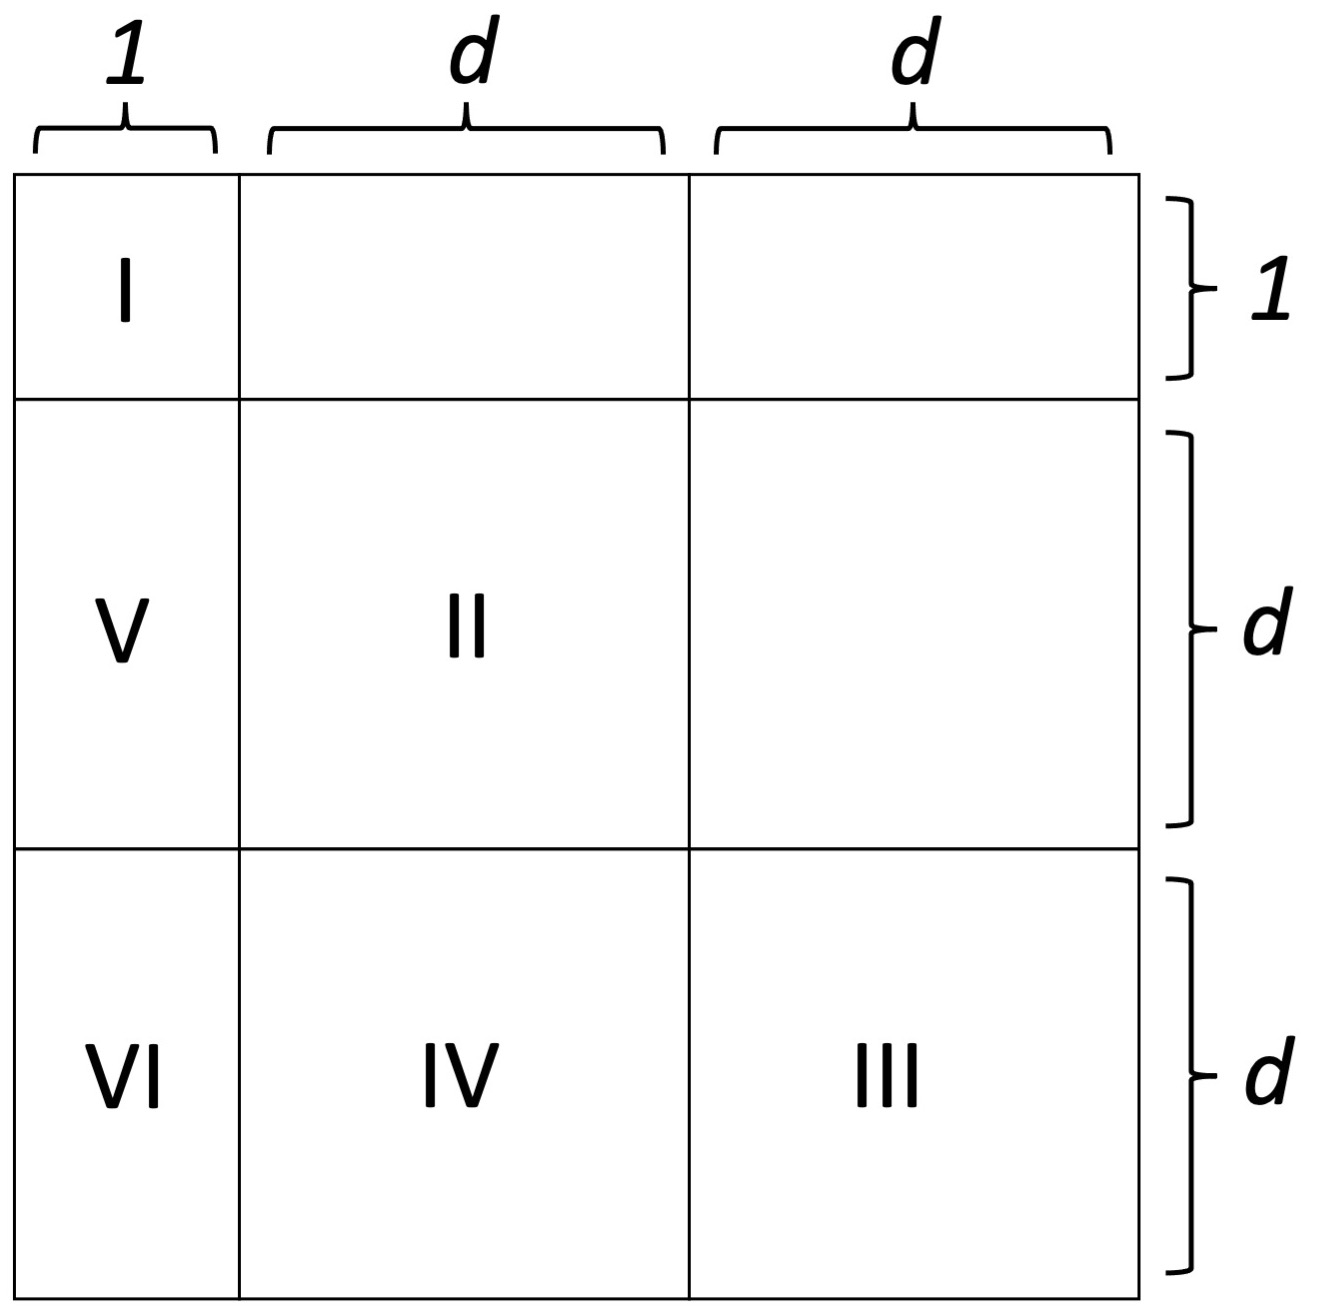
\includegraphics[width=0.45\linewidth]{../../figures/info_matrix/info_matrix_background}
	\caption{Block structure of the observed information matrix $J(\theta; m, g) = -\nabla^2 \mathcal{L}(\theta; m, g)$. The matrix is symmetric, and so we only need to compute submatrices I-VI to compute the entire matrix.}
	\label{infomatrixbackground}
\end{figure}

\subsubsection*{Submatrix I}
Denote submatrix I by $J_{\pi}(\theta; m, g).$ The formula for $J_{\pi}(\theta; m, g)$ is 
\begin{equation}\label{sub_mat_pi}
J_{\pi}(\theta; m, g) = -\E\left[\nabla^2_\pi \mathcal{L}(\theta; m, g, p) \right] + \left(\E\left[ \nabla_\pi \mathcal{L}(\theta; m, g, p) \right] \right)^2 - \E\left[(\nabla_\pi \mathcal{L}(\theta; m, g, p))^2 \right].
\end{equation}

We begin by calculating the first and second derivatives of the log-likelihood $\mathcal{L}$ with respect to $\pi$. The first derivative is
\begin{multline}\label{d_L_d_pi}
\nabla_\pi \mathcal{L}(\theta; m, g, p) = \frac{\partial }{\partial \pi } \left( \sum_{i=1}^n p_i \log(\pi) + \sum_{i=1}^n (1 - p_i) \log(1 - \pi) \right) \\ = \frac{ \sum_{i=1}^n p_i }{\pi} - \frac{ \sum_{i=1}^n (1 - p_i) }{ 1 - \pi } = \frac{\sum_{i=1}^n p_i}{\pi} - \frac{n - \sum_{i=1}^n p_i}{1 - \pi} = \left( \frac{1}{\pi} + \frac{1}{1 - \pi} \right) \sum_{i=1}^n p_i - \frac{n}{1-\pi}.
\end{multline}
The second derivative is
\begin{multline*}
\nabla^2_\pi \mathcal{L}(\theta; m, g, p)  = \frac{\partial^2}{\partial^2\pi} \left( \frac{ \sum_{i=1}^n p_i }{ \pi } - \frac{ n - \sum_{i=1}^n p_i }{1 - \pi}  \right) = \frac{\left( \sum_{i=1}^n p_i \right) - n}{(1 - \pi)^2} - \frac{\sum_{i=1}^n p_i }{ \pi^2 }.
\end{multline*}
We compute the expectation of the first term of (\ref{sub_mat_pi}):
\begin{multline}\label{submat_pi_1}
\E \left[ -\nabla^2_{\pi} \mathcal{L}(\theta; m, g, p)\right] = - \E\left[\frac{ ( \sum_{i=1}^n p_i) - n}{(1 - \pi)^2} - \frac{\sum_{i=1}^n p_i}{\pi^2} \right] \\ = - \E\left\{\left[\frac{1}{(1-\pi)^2} - \frac{1}{\pi^2} \right] \sum_{i=1}^n p_i - \frac{n}{ (1 - \pi)^2 } \right\} \\ = - \left\{\left[ \frac{1}{(1-\pi)^2} - \frac{1}{\pi^2} \right] \sum_{i=1}^n T^\theta_i(1) - \frac{n}{ (1 - \pi)^2}  \right\} \\ = \left[ \frac{1}{\pi^2} - \frac{1}{(1 - \pi)^2} \right] \sum_{i=1}^n T^\theta_i(1) + \frac{n}{(1-\pi)^2}.
\end{multline}
Next, we compute the difference of the second two pieces of (\ref{sub_mat_pi}). To this end, define $$a := \frac{1}{(1-\pi)} + \frac{1}{\pi}$$ and $$b := \frac{n}{(1-\pi)}.$$ We have that
\begin{multline*}
\E \left[\nabla_\pi \mathcal{L}(\theta; m, g, p)^2 \right] \\ = \E \left[ \left( a \sum_{i=1}^n p_i - b\right)^2 \right]  =  \E \left[ a^2 \left( \sum_{i=1}^n p_i \right)^2 - 2ab \sum_{i=1}^n p_i + b^2 \right] \\ = a^2 \sum_{i=1}^n \sum_{j=1}^n \E[p_i p_j] -2ab \sum_{i=1}^n \E [p_i] + b^2.
\end{multline*}
Next,
\begin{equation*}
\left( \E \left[\nabla_\pi \mathcal{L}(\theta; m, g, x) \right] \right)^2 = \left( a \sum_{i=1}^n \E [p_i] - b \right)^2 = a^2 \sum_{i=1}^n \sum_{j=1}^n \E[p_i]  E[p_j] - 2ab \sum_{i=1}^n \E[p_i] + b^2.
\end{equation*}
Therefore,
\begin{multline}\label{submat_pi_2}
(\E [\nabla_\pi \mathcal{L}(\theta; m, g, p)])^2 - \E \left[\nabla_\pi \mathcal{L}(\theta; m, g, p)^2 \right] \\ = a^2 \sum_{i=1}^n \sum_{j=1}^n \E[p_i] \E[p_j] - a^2 \sum_{i=1}^n \sum_{j=1}^n \E[p_i p_j] = a^2 \left( \sum_{i=1}^n \E[p_i]^2 - \E[p_i^2]\right) \\ = a^2 \left( \sum_{i=1}^n [T^\theta_i(1)]^2 - T^\theta_i(1) \right) = \left( \frac{1}{(1 - \pi)} + \frac{1}{\pi} \right)^2 \left(\sum_{i=1}^n [T^\theta_i(1)]^2 - T^\theta_i(1) \right).
\end{multline}
Stringing (\ref{sub_mat_pi}), (\ref{submat_pi_1}) and (\ref{submat_pi_2}) together, we obtain
\begin{multline}\label{sub_mat_1_formula}
J_\pi(\theta; m, g) = 
\left[ \frac{1}{\pi^2} - \frac{1}{(1 - \pi )^2} \right] \sum_{i=1}^n T^\theta_i(1) + \frac{n}{(1-\pi )^2} \\ + \left( \frac{1}{(1 - \pi )} + \frac{1}{\pi} \right)^2 \left( \sum_{i=1}^n [T^\theta_i(1)]^2 - T^\theta_i(1) \right).
\end{multline}

\subsubsection*{Submatrix II}
Denote submatrix II by $J_{\beta^m}(\theta; m, g).$ The formula for $J_{\beta^m}(\theta; m, g)$ is
\begin{multline}\label{sub_mat_2}
J_{\beta^m}(\theta; m, g) = -\E \left[\nabla_{\beta^m}^2 \mathcal{L}(\theta; m, g, p) \right] \\ + \E\left[\nabla_{\beta^m} \mathcal{L}(\theta; m, g, p) \right] \E\left[ \nabla_{\beta^m} \mathcal{L}(\theta; m, g, p) \right]^T - \E\left[ \nabla_{\beta^m} \mathcal{L}(\theta; m, g, p) \nabla_{\beta^m} \mathcal{L}(\theta; m, g, p)^T  \right].
\end{multline}
Standard GLM results imply that
$$ -\nabla_{\beta^m}^2 \mathcal{L}(\theta; m, g, p) = \tilde{X}^T ( \Delta^m V^m \Delta^m - [\Delta']^m H^m ) \tilde{X}$$ and $$\nabla_{\beta^m}\mathcal{L}(\theta; m, g, p) = \tilde{X}^T \Delta^m s^m.$$
We compute the first term of (\ref{sub_mat_2}). The $(k,l)$th entry of this matrix is
\begin{multline*}
\left( \E\left[-\nabla_{\beta^m}^2 \mathcal{L}(\theta; m, g, p)\right]\right)[k,l] = \E \left\{\tilde{X}[,k]^T (\Delta^m V^m \Delta^m - [\Delta']^mH^m) \tilde{X}[,l] \right\} \\ = \sum_{i=1}^n \E \left\{ \tilde{x}_{i,k} (\Delta^m_{i} V^m_{i} \Delta^m_{i} - [\Delta']^m_{i} H^m_{i}) \tilde{x}_{i,l} \right\} \\ = \sum_{i=1}^n \tilde{x}_{i,k}(0) T_i^{\theta}(0) [{\Delta}^m_i(0)  {V}^m_i(0) {\Delta}^m_i(0) - [\Delta']^m_i(0) {H}^m_i(0)] \tilde{x}_{i,l}(0) \\ + \sum_{i=1}^n \tilde{x}_{i,k}(1) T_i^{\theta}(1) [ {\Delta}^m_i(1)  {V}^m_i(1) {\Delta}^m_i(1) - [{\Delta}']^m_i(1) {H}^m_i(1)] \tilde{x}_{i,l}(1) \\ = \sum_{s = 0}^1 \tilde{X}(s)[,k]^T {T}^{\theta}(s) \left[ {\Delta}^m(s) {V}^m(s) {\Delta}^m(s) - [{\Delta}']^m(s) {H}^m(s) \right] \tilde{X}(s)[,l].
\end{multline*}
We therefore have that
\begin{multline}\label{sub_mat_2_1}
\E\left[-\nabla_{\beta^m}^2 \mathcal{L}(\theta; m, g, p)\right] = \sum_{s=0}^1 \tilde{X}(s)^T T^{\theta}(s) \left[ {\Delta}^m(s) {V}^m(s) {\Delta}^m(s) - [{\Delta}']^m(s) {H}^m(s) \right] \tilde{X}(s).
\end{multline}
Next, we compute the difference of the last two terms of (\ref{sub_mat_2}). The $(k,l)$th entry is
\begin{multline*}
\bigg[ \E \left[ \nabla_{\beta^m} \mathcal{L}(\theta; m, g, p) \right] \E \left[ \nabla_{\beta^m} \mathcal{L}(\theta; m, g, p) \right]^T \\ - \E \left[\nabla_{\beta^m} \mathcal{L}(\theta; m, g, p) \nabla_{\beta^m} \mathcal{L}(\theta; m, g, p)^T \right] \bigg] [k,l] \\ 
= \left[ \E \left[\tilde{X}^T \Delta^m s^m \right] \E \left[\tilde{X}^T \Delta^m s^m \right]^T\right][k,l] - \E \left[\tilde{X}^T \Delta^m s^m (s^m)^T \Delta^m \tilde{X} \right][k,l] \\
= \E\left[ \tilde{X}[,k]^T \Delta^m s^m \right] \E \left[ \tilde{X}[,l]^T \Delta^m s^m \right] - \E \left[ \tilde{X}[,k]^T \Delta^m s^m (s^m)^T \Delta^m \tilde{X}[,l ] \right] \\ 
=\E\left(\sum_{i=1}^n \tilde{x}_{ik} \Delta^m_i s^m_{i} \right) \E \left( \sum_{j=1}^n \tilde{x}_{jl} \Delta^m_j s^m_j \right) - \E \left( \sum_{i=1}^n \sum_{j=1}^n \tilde{x}_{ik} \Delta^m_i s^m_i s^m_j \Delta^m_j \tilde{x}_{jl} \right) \\
= \sum_{i=1}^n \sum_{j=1}^n \E[ \tilde{x}_{ik} \Delta^m_is^m_i] \E [\tilde{x}_{jl} \Delta^m_j s^m_j]  -  \sum_{i=1}^n \sum_{j=1}^n \E [ \tilde{x}_{ik} \Delta^m_i s^m_i s^m_j \Delta^m_j \tilde{x}_{jl}] \\
= \sum_{i=1}^n \sum_{j=1}^n \E[ \tilde{x}_{ik} \Delta^m_i s^m_i] \E \left[\tilde{x}_{jl} \Delta^m_j s^m_j \right]  - \sum_{i \neq j} \E [ \tilde{x}_{ik} \Delta^m_i s^m_i] \E[s^m_j \Delta^m_j \tilde{x}_{jl}] \\ - \sum_{i=1}^n \E[\tilde{x}_{ik} \Delta^m_i s^m_i s^m_i \Delta^m_i \tilde{x}_{il}] \\ 
= \sum_{i=1}^n \E[\tilde{x}_{ik} \Delta^m_i s^m_i ] \E [ \tilde{x}_{il} \Delta^m_i s^m_i] - \sum_{i=1}^n \E[\tilde{x}_{ik} (\Delta_i^m)^2 (H_i^m)^2 \tilde{x}_{il}] \\ = \sum_{i=1}^n \left[\tilde{x}_{ik}(0) {\Delta}^m_i(0) T_i^{\theta}(0) {H}^m_i(0) + \tilde{x}_{ik}(1) {\Delta}^m_i(1) T_i^{\theta}(1) {H}^m_i(1) \right] \\ \cdot \left[ \tilde{x}_{il}(0) {\Delta}^m_i(0) T_i^{\theta}(0) {H}^m_i(0) + \tilde{x}_{il}(1) {\Delta}^m_i(1) T_i^{\theta}(1) {H}^m_i(1) \right] \\ - \sum_{i=1}^n \left[ \tilde{x}_{ik}(0) T_i^{\theta}(0) (\Delta_i^m(0))^2 ({H}_i^m(0))^2 \tilde{x}_{il}(0)  + \tilde{x}_{ik}(1) T_i^{\theta}(1) ({\Delta}^m_i(1))^2 ({H}_i^m(1))^m \tilde{x}_{il}(1) \right] \\ = \sum_{s=0}^1 \sum_{t=0}^1 \left[ \sum_{i=1}^n \tilde{x}_{ik}(s) T^{\theta}_i(s) {\Delta}^m_i(s) {H}^m_i(t) T_i^{\theta}(t){\Delta}^m_i(t) {H}^m_i(t) \tilde{x}_{il}(t) \right] \\ - \sum_{s=0}^1 \left[\sum_{i=1}^n \tilde{x}_{ik}(s) T_i^\theta(s) ({\Delta}^m_i(s))^2 ({H}_i^m(s))^2 \tilde{x}_{il}(s) \right] \\ = \sum_{s=0}^1 \sum_{t=0}^1 \tilde{X}(s)[,k]^T {T}^\theta(s) {\Delta}^m(s) {H}^m(s) {T}^\theta(t) {\Delta}^m(t) {H}^m(t) \tilde{X}(k)[,l] \\ - \sum_{s=0}^1{X}(s)[,k]^T {T}^\theta(s) ({\Delta}^m(s))^2 ({H}^m(s))^2 \tilde{X}(s)[,l].
\end{multline*}
The sum of the last two terms on the right-hand side of (\ref{sub_mat_2}) is therefore
\begin{multline}\label{sub_mat_2_2}
 \E \left[ \nabla_{\beta^m} \mathcal{L}(\theta; m, g, p) \right] \E \left[ \nabla_{\beta^m} \mathcal{L}(\theta; m, g, p) \right]^T - \E \left[\nabla_{\beta^m} \mathcal{L}(\theta; m, g, p) \nabla_{\beta^m} \mathcal{L}(\theta; m, g, p)^T \right] \\ =
\sum_{s=0}^1 \sum_{t=0}^1 \tilde{X}(s)^T {T}^\theta(s) {\Delta}^m(s) {H}^m(s) T^{\theta}(t) {\Delta}^m(t) {H}^m(t) \tilde{X}(t) \\ - \sum_{s=0}^1 \tilde{X}(s)^T {T}^\theta(s) ({\Delta}^m(s))^2 ({H}^m(s))^2 \tilde{X}(s). \end{multline}
Combining (\ref{sub_mat_2}), (\ref{sub_mat_2_1}), (\ref{sub_mat_2_2}), we find that
\begin{multline}\label{sub_mat_2_formula}
J_{\beta^m}(\theta; m, g) = \sum_{s=0}^1 \tilde{X}(s)^T T^{\theta}(s) \left[ {\Delta}^m(s) {V}^m(s) {\Delta}^m(s) - [{\Delta}']^m(s) {H}^m(s) \right] \tilde{X}(s) \\ + \sum_{s=0}^1 \sum_{t=0}^1 \tilde{X}(s)^T {T}^\theta(s) {\Delta}^m(s) {H}^m(s) {T}^\theta(t) {\Delta}^m(t) {H}^m(t) \tilde{X}(t) \\ - \sum_{s=0}^1 \tilde{X}(s)^T T^{\theta}(s) ({\Delta}^m(s))^2 ({H}^m(s))^2 \tilde{X}(s).
\end{multline}

\subsubsection*{Submatrix III}
Denote submatrix III by $J_{\beta^g}(\theta; m, g).$ The formula for sub-matrix III is similar to that of sub-matrix II (\ref{sub_mat_2_formula}). Substituting $g$ for $m$ in this equation yields
\begin{multline}\label{sub_mat_3_formula}
J_{\beta^g}(\theta; m, g) = \sum_{s=0}^1 \tilde{X}(s)^T T^{\theta}(s) \left[{\Delta}^g(s) {V}^g(s) {\Delta}^g(s) - [{\Delta}']^g(s) {H}^g(s) \right] \tilde{X}(s) \\ + \sum_{s=0}^1 \sum_{t=0}^1 \tilde{X}(s)^T {T}^\theta(s) {\Delta}^g(s) {H}^g(s) {T}^\theta(t) {\Delta}^g(t) {H}^g(t) \tilde{X}(t) \\ - \sum_{s=0}^1 \tilde{X}(s)^T T^{\theta}(s) ({\Delta}^g(s))^2 ({H}^g(s))^2 \tilde{X}(s).
\end{multline}

\subsubsection*{Submatrix IV}
Denote sub-matrix IV by $J_{(\beta^g, \beta^m)}(\theta; m, g)$. The formula for $J_{(\beta^g, \beta^m)}(\theta; m, g)$ is 
\begin{multline}\label{sub_mat_4}
J_{(\beta^g, \beta^m)}(\theta; m,g) = \E \left[-\nabla_{\beta^g} \nabla_{\beta^m} \mathcal{L}(\theta; m, g, p) \right] \\ + \E\left[ \nabla_{\beta^{g}}\mathcal{L}(\theta ; m,g,p) \right] \E \left[\nabla_{\beta^m}\mathcal{L} (\theta ; m,g,p)  \right]^T - \E \left[ \nabla_{\beta^{g}}\mathcal{L} (\theta; m,g,p) \nabla_{\beta^m}\mathcal{L}(\theta; m,g,p)^T  \right].
\end{multline}
First, we have that
\begin{equation}\label{sub_mat_4_1}
\E\left[-\nabla_{\beta^g} \nabla_{\beta^m} \mathcal{L}(\theta; m, g, p) \right] = 0,
\end{equation}
as differentiating $\mathcal{L}$ with with respect to $\beta^g$ yields a vector that is a function of $\beta^g$, and differentiating this vector with respect to $\beta^m$ yields $0$. Next, recall from GLM theory that $\nabla_{\beta^g} \mathcal{L}(\theta; m, g, p) =   \tilde{X}^T\Delta^g s^g$ and $\nabla_{\beta^m} \mathcal{L}(\theta; m, g, p) = \tilde{X}^T \Delta^m s^m.$ The $(k,l)$th entry of the last two terms of (\ref{sub_mat_4}) is
\begin{multline}\label{sub_mat_4_2}
\bigg[ \E \left[\nabla_{\beta^g} \mathcal{L}(\theta; m, g, p) \right] \E \left[\nabla_{\beta^m} \mathcal{L}(\theta; m, g, p) \right]^T \\ - \E \left[ \nabla_{\beta^g} \mathcal{L}(\theta; m, g, p) \nabla_{\beta^m} \mathcal{L}(\theta; m, g, p)^T \right] \bigg][k,l] \\ 
= \left[ \E \left[ \tilde{X}^T \Delta^g s^g \right]\E \left[ \tilde{X}^T \Delta^m s^m \right]^T\right][k,l] - \E \left[ \tilde{X}^T \Delta^g s^g (s^m)^T \Delta^m \tilde{X} \right][k,l] \\ 
= \E\left[\tilde{X}[,k]^T \Delta^g s^g \right] \E \left[\tilde{X}[,l]^T \Delta^m s^m \right] - \E \left[\tilde{X}[,k]^T \Delta^g s^g (s^m)^T \Delta^m \tilde{X}[,l ] \right] \\
=\E\left( \sum_{i=1}^n \tilde{x}_{ik} \Delta^g_i s^g_i \right) \E \left( \sum_{j=1}^n \tilde{x}_{jl} \Delta^m_j s^m_j \right) - \E \left( \sum_{i=1}^n \sum_{j=1}^n \tilde{x}_{ik} \Delta^g_i s^g_i s^m_j \Delta^m_j \tilde{x}_{jl} \right) \\ 
= \sum_{i=1}^n \sum_{j=1}^n \E[\tilde{x}_{ik} \Delta^g_is^g_i] \E[ \tilde{x}_{jl} \Delta^m_j s^m_j ] - \sum_{i=1}^n \sum_{j=1}^n \E[ \tilde{x}_{ik} \Delta^g_i s^g_i s^m_j \Delta^m_j \tilde{x}_{jl}]  \\
= \sum_{i=1}^n \sum_{j=1}^n \E[ \tilde{x}_{ik} \Delta^g_i s^g_i] \E \left[\tilde{x}_{jl} \Delta^m_j s^m_j \right]  - \sum_{i \neq j} \E[\tilde{x}_{ik} \Delta^g_i s^g_i] \E[\tilde{x}_{jl}\Delta^m_j  s^m_j ] \\ - \sum_{i=1}^n \E[\tilde{x}_{ik} \Delta^g_i s^g_i s^m_i \Delta^m_i \tilde{x}_{il}] \\
= \sum_{i=1}^n \E[\tilde{x}_{ik} \Delta^g_i H^g_i] \E[\tilde{x}_{il} \Delta_i^m H^m_i] - \sum_{i=1}^n \E[\tilde{x}_{ik} H_i^g \Delta_i^g \Delta_i^m H_i^m \tilde{x}_{il}] \\ 
= \sum_{i=1}^n \left[\tilde{x}_{ik}(0) {\Delta}^g_i(0) T^\theta_i(0) {H}^g_i(0) + \tilde{x}_{ik}(1) {\Delta}^g_i(1) T^\theta_i(1) {H}^g_i(1)\right] \\ 
\cdot \left[\tilde{x}_{il}(0) {\Delta}^m_i(0) T^\theta_i(0) {H}^m_i(0) + \tilde{x}_{il}(1) {\Delta}^m_i(1) T^\theta_i(1) {H}^m_i(1)\right] 
\\ - \sum_{i=1}^n [\tilde{x}_{ik}(0) T^\theta_i(0) {\Delta}^g_i(0) {H}^g_i(0) {\Delta}^m_i(0) {H}^m_i(0) \tilde{x}_{il}(0) \\ + \tilde{x}_{ik}(1) T^\theta_i(1) {\Delta}^g_i(1) {H}^g_i(1) {\Delta}^m_i(1) {H}^m_i(1) \tilde{x}_{il}(1) ] 
\\ = \sum_{s=0}^1 \sum_{t=0}^1 \left[\sum_{i=1}^n \tilde{x}_{ik}(s) T^\theta_i(s) {\Delta}^g_i(s) {H}^g_i(s) T^\theta_i(t){\Delta}^m_i(t) {H}^m_i(t) \tilde{x}_{il}(t) \right]
\\ - \sum_{s=0}^1 \left[\sum_{i=1}^n \tilde{x}_{ik}(s) T^\theta_i(s) {\Delta}^g_i(s) {H}^g_i(s) {\Delta}^m_i(s) {H}^m_i(s) \tilde{x}_{il}(s)\right] 
\\ = \sum_{s=0}^1 \sum_{t=0}^1 \left[ \tilde{X}(s)[,k]^T T^\theta(s) {\Delta}^g(s) {H}^g(s) T^\theta(t){\Delta}^m(t) {H}^m(t) \tilde{X}(t)[,l] \right]\\ - \sum_{s=0}^1 \left[ \tilde{X}[,k]^T T^\theta(s) {\Delta}^g(s) {H}^g(s) {\Delta}^m(s) {H}^m(s) \tilde{X}[,l](s)\right].
\end{multline}
Combining (\ref{sub_mat_4}), (\ref{sub_mat_4_1}), and (\ref{sub_mat_4_2}) produces
\begin{multline}\label{sub_mat_4_formula}
J_{(\beta^g, \beta^m)}(\theta; m, g) = \sum_{s=0}^1 \sum_{t=0}^1 \tilde{X}(s)^T  T^\theta(s) {\Delta}^g(s) {H}^g(s) T^\theta(t){\Delta}^m(t) {H}^m(t) \tilde{X}(t) \\ - \sum_{s=0}^1 \tilde{X}(s)^T T^\theta(s) {\Delta}^g(s) {H}^g(s) {\Delta}^m(s) {H}^m(s) \tilde{X}(s).
\end{multline}
\subsubsection*{Submatrix V}
Denote submatrix V by $J_{(\beta^m,\pi)}(\theta; m, g).$ The formula for $J_{(\beta^m,\pi)}(\theta; m, g)$ is
\begin{multline}\label{sub_mat_5}
J_{(\beta^m,\pi)}(\theta; m, g) = \E \left[ - \nabla_{\beta^m} \nabla_{ \pi } \mathcal{L}(\theta; m, g, p) \right] \\ + \E\left[ \nabla_{\beta^m}\mathcal{L}(\theta ; m,g,p) \right] \E \left[ \nabla_{\pi}\mathcal{L}(\theta ; m,g,p) \right]^T  - \E \left[ \nabla_{\beta^m}\mathcal{L}(\theta; m,g,p) \nabla_{\pi}\mathcal{L}(\theta; m,g,p)^T \right].
\end{multline}
We have that
\begin{equation}\label{sub_mat_5_1}
\E \left[ - \nabla_{\beta^m} \nabla_{ \pi } \mathcal{L}(\theta; m, g, p) \right] = 0,
\end{equation}
as $\beta^m$ and $\pi$ separate in the log likelihood. Next, set $a := 1/\pi + 1/(1 - \pi)$ and $b := n/(1 - \pi).$ Recall from GLM theory that
$\nabla_{\beta^m} \mathcal{L}(\theta; m, g, p) = \tilde{X}^T \Delta^m s^m$ and from (\ref{d_L_d_pi}) that
$a \sum_{i=1}^n p_i - b.$
The $k$th entry of the last two terms of (\ref{sub_mat_5}) is
\begin{multline}\label{sub_mat_5_2}
\E \left[\nabla_\pi \mathcal{L}(\theta; m, g, p) \right] \E\left[\nabla_{\beta^m} \mathcal{L}(\theta; m, g, p)[k] \right] - \E \left[\nabla_{\pi}\mathcal{L}(\theta; m,g,p) \nabla_{\beta^m}\mathcal{L}(\theta; m,g,p)[k] \right] \\= \left(\E \left[ a \sum_{i=1}^n p_i - b \right] \right) \left(\E\left[ \tilde{X}[,k]^T \Delta^m s^m \right] \right) - \E \left[ \left( a \sum_{i=1}^n p_i - b \right) \tilde{X}[,k]^T \Delta^m s^m \right] \\ = \left( a \sum_{i=1}^n \E[p_i] - b \right) \left( \sum_{j=1}^n \E [ \tilde{x}_{jk}\Delta^m_js^m_j] \right) - \E \left[ \left( a \sum_{i=1}^n p_i - b \right) \left( \sum_{j=1}^n \tilde{x}_{jk} \Delta^m_j s^m_j \right) \right] \\ = a \sum_{i=1}^n \sum_{j=1}^n \E [p_i] \E[ \tilde{x}_{jk} \Delta^m_j s^m_j] - b \sum_{j=1}^n \E[\tilde{x}_{jk} \Delta^m_j s^m_j] \\ - \left[ a \sum_{i=1}^n \sum_{j=1}^n \E [ p_i \tilde{x}_{jk} \Delta^m_j s^m_j] - b \sum_{j=1}^n \E[\tilde{x}_{jk} \Delta^m_j s^m_j] \right] \\ =  a \sum_{i=1}^n \sum_{j=1}^n \E[p_i] \E[\tilde{x}_{jk} \Delta^m_j s^m_j] - a\sum_{i \neq j} \E[p_i] \E[\tilde{x}_{jk} \Delta^m_j s^m_j] - a\sum_{i=1}^n \E[ p_i \tilde{x}_{ik} \Delta^m_i s^m_i ] \\ = a \sum_{i=1}^n \E[p_i] \E[ \tilde{x}_{ik} \Delta^m_i s^m_i] - a \sum_{i=1}^n \E[p_i \tilde{x}_{ik} \Delta^m_i s^m_i] \\ = a \sum_{i=1}^n T^\theta_i(1) [T^\theta_i(0) \Delta^m_i(0) s^m_i(0) \tilde{x}_{ik}(0) + T^\theta_i(1) \Delta^m_i(1) s^m_i(1) \tilde{x}_{ik}(1)] \\ - a \sum_{i=1}^n T^\theta_i(1)\Delta^m_i(1)s^m_i(1)\tilde{x}_{ik}(1) \\ = a \sum_{i=1}^n T^\theta_i(0)T^\theta_i(1) \Delta_i^m(0)H^m_i(0)\tilde{x}_{ik}(0) \\ + a \sum_{i=1}^n \left( [T^\theta_i(1)]^2 \Delta^m_i(1)H^m_i(1) - T^\theta_i(1)\Delta^m_i(1)H^m_i(1) \right) \tilde{x}_{ik}(1)  \\ =a \left[ \sum_{i=1}^n T^\theta_i(0) T^\theta_i(1) \Delta^m_i(0) H^m_i(0) \tilde{x}_{ik}(0) + \sum_{i=1}^n T^\theta_i(1)\Delta^m_i(1)H^m_i(1)[T^\theta_i(1) - 1] \tilde{x}_{ik}(1) \right] \\ = a \left[ \sum_{i=1}^n T^\theta_i(0) T^\theta_i(1) \Delta^m_i(0) H^m_i(0) \tilde{x}_{ik}(0) - \sum_{i=1}^n T^\theta_i(0) T^\theta_i(1) \Delta^m_i(1) H^m_i(1) \tilde{x}_{ik}(1) \right] \\ = a\left(\tilde{X}(0)[,k]^T w^m(0) - \tilde{X}(1)[,k]^T w^m(1)  \right).
\end{multline}
Combining (\ref{sub_mat_5}), (\ref{sub_mat_5_1}), and (\ref{sub_mat_5_2}), we conclude that
\begin{equation}\label{sub_mat_5_formula} J_{(\beta^m, \pi)}(\theta; m, g, p) = \left( \frac{1}{\pi} + \frac{1}{1 - \pi} \right) \left( \tilde{X}(0)^T w^m(0) - \tilde{X}(1)^T w^m(1)\right). \end{equation}

\subsubsection*{Submatrix VI}
Denote submatrix VI by $J_{(\beta^g,\pi)}(\theta; m, g).$ Calculations similar to those for submatrix V show that
\begin{equation}\label{sub_mat_6_formula} J_{(\beta^g, \pi)}(\theta; m, g, p) = \left(\frac{1}{\pi} + \frac{1}{1 - \pi} \right) \left( \tilde{X}(0)^T w^g(0) - \tilde{X}(1)^T w^g(1)\right). \end{equation}

\subsubsection*{Combining submatrices}
To summarize, the formulas for submatrices I-VI are as follows:
\begin{itemize}
\item[I]\begin{multline*}
J_\pi(\theta; m, g) = 
\left[ \frac{1}{\pi^2} - \frac{1}{(1 - \pi )^2} \right] \sum_{i=1}^n T^\theta_i(1) + \frac{n}{(1-\pi )^2} \\ + \left( \frac{1}{(1 - \pi )} + \frac{1}{\pi} \right)^2 \left( \sum_{i=1}^n [T^\theta_i(1)]^2 - T^\theta_i(1) \right).
\end{multline*}
\item[II] \begin{multline*}
J_{\beta^m}(\theta; m, g) = \sum_{s=0}^1 \tilde{X}(s)^T T^{\theta}(s) \left[ {\Delta}^m(s) {V}^m(s) {\Delta}^m(s) - [{\Delta}']^m(s) {H}^m(s) \right] \tilde{X}(s) \\ + \sum_{s=0}^1 \sum_{t=0}^1 \tilde{X}(s)^T {T}^\theta(s) {\Delta}^m(s) {H}^m(s) {T}^\theta(t) {\Delta}^m(t) {H}^m(t) \tilde{X}(t) \\ - \sum_{s=0}^1 \tilde{X}(s)^T T^{\theta}(s) ({\Delta}^m(s))^2 ({H}^m(s))^2 \tilde{X}(s).
\end{multline*}
\item[III] \begin{multline*}
J_{\beta^g}(\theta; m, g) = \sum_{s=0}^1 \tilde{X}(s)^T T^{\theta}(s) \left[{\Delta}^g(s) {V}^g(s) {\Delta}^g(s) - [{\Delta}']^g(s) {H}^g(s) \right] \tilde{X}(s) \\ + \sum_{s=0}^1 \sum_{t=0}^1 \tilde{X}(s)^T {T}^\theta(s) {\Delta}^g(s) {H}^g(s) {T}^\theta(t) {\Delta}^g(t) {H}^g(t) \tilde{X}(t) \\ - \sum_{s=0}^1 \tilde{X}(s)^T T^{\theta}(s) ({\Delta}^g(s))^2 ({H}^g(s))^2 \tilde{X}(s).
\end{multline*}
\item[IV] \begin{multline*}
J_{(\beta^g, \beta^m)}(\theta; m, g) = \sum_{s=0}^1 \sum_{t=0}^1 \tilde{X}(s)^T  T^\theta(s) {\Delta}^g(s) {H}^g(s) T^\theta(t){\Delta}^m(t) {H}^m(t) \tilde{X}(t) \\ - \sum_{s=0}^1 \tilde{X}(s)^T T^\theta(s) {\Delta}^g(s) {H}^g(s) {\Delta}^m(s) {H}^m(s) \tilde{X}(s).
\end{multline*}
\item[V] $$ J_{(\beta^m, \pi)}(\theta; m, g, p) = \left( \frac{1}{\pi} + \frac{1}{1 - \pi} \right) \left( \tilde{X}(0)^T w^m(0) - \tilde{X}(1)^T w^m(1)\right).  $$
\item[VI] $$ J_{(\beta^g, \pi)}(\theta; m, g, p) = \left(\frac{1}{\pi} + \frac{1}{1 - \pi} \right) \left( \tilde{X}(0)^T w^g(0) - \tilde{X}(1)^T w^g(1)\right).$$
\end{itemize}
We stitch these pieces together and transpose submatrices IV, V, and VI to produce the whole information matrix $J(\theta; m, g)$. Evaluating this matrix at the EM estimate $\theta^\textrm{EM}$ and inverting yields the asymptotic covariance matrix, which we can use to compute standard errors.

\subsection{Implementation}
To evaluate the observed information matrix, we need to compute the matrices $\Delta^m(j),$ $[\Delta']^m(j),$ $V^m(j),$ and $H^m(j)$ and the vectors $s^m(j)$ and $w^m(j)$ for $j \in \{0,1\}$. We likewise need to compute the analogous gRNA quantities. We describe how to compute these quantities in R by extending base family objects. We implicitly condition on $p_i$, $z^m_i$, and $o^m_i$.

\begin{algorithm}
	\caption{Computing the matrices $\Delta^m(j)$, $[\Delta']^m(j)$, $V^m(j)$, $H^m(j)$, and $s^m(j)$ given given $\beta_m$.}\label{algo:computing_info_matrices}
	\begin{algorithmic}[3]
		\Require A coefficient vector $\beta_m$; data $[m_1, \dots, m_n]$, $[o^m_1, \dots, o^m_n]$, and $[z_1, \dots, z_n]$; and a family object containing functions \texttt{linkinv}, \texttt{variance}, \texttt{mu.eta}, \texttt{mu.eta.prime}, and \texttt{skewness}.
		\For{$j \in \{0, 1\}$}
		\For{$i \in \{1, \dots, n\}$}
		\State $l^m_i(j) \gets \langle \beta_m, \tilde{x}_i(j) \rangle + o^m_i$
		\State $\mu^m_i(j) \gets \texttt{linkinv}(l^m_i(j))$
		\State $[\sigma_i^m(j)]^2 \gets \texttt{variance}(\mu_i^m(j))$
		\State $h_m'(l_i^m(j)) \gets \texttt{mu.eta}(l_i^m(j))/[\sigma_i^m(j)]^2$
		\State $\gamma^m_i(j) \gets \texttt{skewness}(\mu^m_i(j))$
		\State $[r_m^{-1}]''(l_i^m(j)) \gets \texttt{mu.eta.prime}(l^m_i(j))$
		\State $$h_m''(l_i^m(j)) \gets \frac{[r^{-1}]''(l_i^m(j)) - [([\sigma_i^m(j)]^2)^{3/2}][\gamma^m_i(j)] [h_m'(l_i^m(j))]^2}{[\sigma_i^m(j)]^2}$$
		\Comment Assign quantities to matrices
		\State $\Delta_{i}^m(j) \gets h_m'( l_i^m(j))$
		\State $[\Delta']^m_{i}(j) \gets h''(l^m_i(j))$
		\State $V^m_{i}(j) \gets [\sigma^m_i(j)]^2$
		\State $H^m_{i}(j) \gets s^m_i(j) \gets m_i - \mu^m_i(j)$
		\EndFor
		\EndFor
	\end{algorithmic}
\end{algorithm}

An \texttt{R} family object contains several functions, including \texttt{linkinv}, \texttt{variance}, and \texttt{mu.eta}. \texttt{linkinv} is the inverse link function $r_m^{-1}$. \texttt{variance} takes as an argument the mean $\mu^m_i$ and returns the variance $[\sigma_i^m]^2$. \texttt{mu.eta} is the derivative of the inverse link function $[r^{-1}_m]^{'}$. We extend the \texttt{R} family object by adding two additional functions: \texttt{skewness} and \texttt{mu.eta.prime}. \texttt{skewness} returns the skewness $\gamma^m_i$ of the distribution as a function of the mean $\mu_i$, i.e. $$\texttt{skewness}\left(\mu_i\right) = \E \left[\left(\frac{m_i - \mu_i^m}{ \sigma_i^m}\right)^3\right] := \gamma_i^m.$$ Finally, the \texttt{mu.eta.prime} is the second derivative of the inverse link function $[r^{-1}_m]''.$ Algorithm \ref{algo:computing_info_matrices} computes the matrices $\Delta^m(j)$, $[\Delta']^m(j)$, $V^m(j)$, $H^m(j)$, and vector $s^m(j)$ for given $\beta_m$ and given family object. (The vector $w^m(j)$ can be computed in terms of $\Delta^m(j)$ and $H^m(j)$.) We use $\sigma^m_i(j)$ (resp. $\gamma^m_i(j)$) to refer to the standard deviation (resp. skewness) of the gene expression distribution the $i$th cell when the perturbation $p_i$ is set to $j$.

All steps of the algorithm are obvious except the calculation of $h'_m(l^m_i(j))$ (line 6), $h''(l^m_i(j))$ (line 9), and $V^m_i(j)$ (line 12). We omit the $(j)$ notation for compactness. First, we prove the correctness of the expression for $h'_m(l^m_i)$. Recall the basic GLM identities
\begin{equation}\label{computing_info_matrix_1}
\psi_m''(\eta_i^m) =  [\sigma^m_i]^2
\end{equation}
 and, for all $t \in \R$, 
\begin{equation}\label{computing_info_matrix_2}
 r_m^{-1}(t) = \psi_m'(h_m(t)).
\end{equation}
 Differentiating (\ref{computing_info_matrix_2}) in $t$, we find that
\begin{equation}\label{computing_info_matrix_3}
 (r_m^{-1})'(t) = \psi_m''(h_m(t))h_m'(t), 
\end{equation}
or  $$h_m'(t) = \frac{(r_m^{-1})'(t) }{\psi_m''(h_m(t))}.$$ Finally, plugging in $l^m_i$ for $t$,
$$ h_m'(l_i) = \frac{(r_m^{-1})'(l^m_i)}{\psi''(h_m(l^m_i))} = \frac{(r_m^{-1})'(l^m_i)}{\psi_m''(\eta^m_i)} = \textrm{ by (\ref{computing_info_matrix_1}) } \frac{(r_m^{-1})'(l_i^m)}{[\sigma_i^m]^2}.$$

Next, we prove the correctness for the expression for $h_m''(l_i^m)$. Recall the exponential family identity 
\begin{equation}\label{computing_info_matrix_4}
\psi'''_m(\eta^m_i) = \gamma^m_i  ([\sigma^m_i]^2)^{3/2}.
\end{equation}
Differentiating (\ref{computing_info_matrix_3}) in $t$, we obtain
$$ (r_m^{-1})''(t) = \psi_m'''(h_m(t)) [h_m'(t)]^2 + \psi_m''(h_m(t)) h_m''(t),$$ or $$h_m''(t) =\frac{(r_m^{-1})''(t) - \psi'''(h_m(t))[h_m'(t)]^2}{\psi_m''(h_m(t))}.$$ Plugging in $l^m_i$ for $t$, we find that
\begin{equation*}
h_m''(l^m_i) = \frac{(r_m^{-1})''(l^m_i) - \psi_m'''(\eta^m_i) [h_m'(l_i^m)]^2}{[\sigma_i^m]^2} = \textrm{ (by \ref{computing_info_matrix_4}) }  \frac{(r_m^{-1})''(l^m_i) - ([\sigma_i^m]^2)^{3/2} (\gamma_i^m) [h_m'(l^m_i)]^2 }{[\sigma_i^m]^2}.
\end{equation*}
Finally, the expression for $V^m_i$ follows from (\ref{computing_info_matrix_1}). We can apply a similar algorithm to compute the analogous matrices for the gRNA modality. Table \ref{family_object_functions} shows the \texttt{linkinv}, \texttt{variance}, \texttt{mu.eta}, \texttt{skewness}, and \texttt{mu.eta.prime} functions for several common family objects (which are defined by a distribution and link function). 
\begin{table}
\centering
\caption{\texttt{linkinv}, \texttt{variance}, \texttt{mu.eta}, \texttt{skewness}, \texttt{mu.eta.prime} for common family objects (i.e., pairs of distributions and link functions).}\label{family_object_functions}
\begin{tabular}{|C{2.5cm}|C{3.5cm}|C{3.4cm}|C{2.5cm}|}
	\hline 
	& Gaussian response, identity link & Poisson response, log link & NB response ($\theta > 0$ fixed), log link \\ 
	\hline 
	\texttt{linkinv} & $x$ & $\exp(x)$ & $\exp(x)$  \\ 
	\hline 
	\texttt{variance} & $x$ & $x$ & $x + x^2/\theta$ \\ 
	\hline 
	\texttt{mu.eta} & $1$ & $x$  & $\exp(x)$ \\ 
	\hline 
	\texttt{skewness} & $0$ & $x^{-1/2}$ & $\frac{2 x + \theta}{\sqrt{\theta x} \sqrt{x + \theta}}$ \\ 
	\hline 
	\texttt{mu.eta.prime} & $0$ & $\exp(x)$ & $\exp(x)$ \\ 
	\hline 
\end{tabular}
\end{table}

\section{Zero-inflated model}\label{sec:zero_inf_model}
In this section we introduce the ``zero-inflated'' GLM-EIV model. The zero-inflated GLM-EIV model is appropriate to use when the unperturbed cells do not transcribe \textit{any} gRNA molecules (i.e., when there are no background reads). Let $x_i = [1, z_i]^T \in \R^{d-1}$ be the vector of observed covariates, including an intercept term. ($x_i$ is the same as $\tilde{x}_i$, but with the perturbation indicator $p_i$ removed.) Let $\beta_{g,z} = [\beta^g_0, \gamma_g] \in \R^{d-1}$ be an unknown coefficient vector. ($\beta_{g,z}$ is the same as $\beta_g$, but with the perturbation effect $\beta^g_1$ removed). Let the linear component $l^{g,z}_i$, mean $\mu^{g,z}_i$, and canonical parameter $\eta^{g,z}_i$ of gRNA count distribution of the $i$th cell be given by
$$
l^{g,z}_i = \langle x_i, \beta_{g,z} \rangle + o^g_i; \quad
r_g(\mu^{g,z}_i) = l^{g,z}_i; \quad
\eta^{g,z}_i = ([\psi'_g]^{-1} \circ r^{-1}_g)(l^{g,z}_i) := h_g(l^{g,z}_i).
$$
The density $f_{g,z}$ of gRNA counts in the zero-inflated model is as follows:
$$f_{g,z}(g_i; \eta^{g,z}_i, p_i) = [f_g(g_i;\eta^{g,z}_i)]^{p_i} \mathbb{I}(g_i = 0)^{1-p_i}.$$
In other words, when the cell is \textit{perturbed} (i.e., $p_i = 1$), the zero-inflated density $f_{g,z}$ coincides with the background-read density $f_g$; by contrast, when the cell is \textit{unperturbed} (i.e., $p_i = 0$), the zero-inflated density $f_{g,z}$ is a point mass at zero. The gene expression density $f_m$ and perturbation indicator density $f_p$ are the same across the background read and zero-inflated models. We assume that the gene expression $m_i$ and gRNA count $g_i$ are conditionally independent given the perturbation indicator $p_i$. The joint density $f_z$ of $(m_i, p_i, z_i)$ is
\begin{equation*}
f_z(m_i, g_i, p_i) = f_m(m_i | p_i) f_{g,z}(g_i | p_i) f_p(p_i) = \pi^{p_i} (1-\pi)^{1-p_i} f_m(m_i; \eta^m_i)[f_g(g_i; \eta_i^{g,z})]^{p_i} \mathbb{I}(g_i = 0)^{1-p_i}.
\end{equation*}
The complete-data log-likelihood $\mathcal{L}_z$ is
\begin{multline*}
\mathcal{L}_z(\theta; m, g, p) = \sum_{i=1}^n \log \left[ \pi^{p_i} (1-\pi)^{1-p_i} \right] + \sum_{i=1}^n \log\left[f_m(m_i; \eta^m_i) \right] \\ + \sum_{i=1}^n p_i \log \left[f_{g}(g_i; \eta_i^{g,z}) \right] + \sum_{i=1}^n (1 - p_i)\log\left[ \mathbb{I}(g_i = 0) \right],
\end{multline*}
where $\theta = [\pi, \beta_m, \beta_{g,z}]$ is the vector of unknown parameters.
Integrating over the unobserved variable $p_i$, the marginal $f_z$ of $(m_i, g_i)$ is
$$f_z(m_i, g_i; \theta) = (1-\pi) f_m(m_i;\eta^m_i(0)) \mathbb{I}(g_i = 0) + \pi f_m(m_i; \eta^m_i(1)) f_g(g_i;\eta^{g,z}_i).$$ Finally, the log-likelihood is
$$
\mathcal{L}_z(\theta; m_i, g_i) = \sum_{i=1}^n \log\left[ (1-\pi) f_m(m_i;\eta^m_i(0)) \mathbb{I}(g_i = 0) + \pi f_m(m_i; \eta^m_i(1)) f_g(g_i;\eta^{g,z}_i) \right].
$$

\subsection{Estimation}
To estimate the parameters of the zero-inflated GLM-EIV model, we use an EM algorithm similar to Algorithm \ref{algo:em_full} but with two changes. First, we use a different formula for the $i$th membership probability at the $t$-th step of the algorithm $T^{(t)}_i(1)$. (We use $T^{(t)}_i(1)$ to denote the $i$th membership probability in \textit{both} the background read and zero inflated cases; the difference should be clear from context.) Let $\theta^{(t)} = (\pi^{(t)}, \beta^{(t)}_m, \beta^{(t)}_{g,z})$ be the parameter estimate at the $t$-th iteration of the algorithm. Arguing in a manner similar to the background read case, we have that $$T^{(t)}_i(1) = \frac{1}{ \exp(q_i^{\left(t,z\right)}) + 1},$$ where
$$q_i^{(t,z)} = \log \left(\frac{(1 - \pi^{(t)}) \P(M_i = m_i | P_i = 0, \theta^{(t)}) \P(G_i = g_i | P_i = 0, \theta^{(t)})}{(\pi^{(t)}) \P(M_i = m_i | P_i = 1, \theta^{(t)}) \P(G_i = g_i | P_i = 1, \theta^{(t)})}\right).$$
The expression for $q^{(t,z)}_i$ is
\begin{multline*}
q^{(t,z)}_i = \log\left[ 1 - \pi^{(t)} \right] + \log\left[ f_m\left(m_i; \left[ \eta^m_i(0) \right]^{(t)}\right) \right] + \log\left[ \mathbb{I}(g_i = 0) \right] \\ - \log\left[ \pi^{(t)} \right] - \log\left[ f_m\left(m_i; \left[ \eta^m_i(1) \right]^{(t)}\right) \right] - \log\left[ f_g\left(g_i; \left[\eta^{g,z}_i \right]^{(t)}\right) \right],
\end{multline*}
where $[\eta^{g,z}_i]^{(t)} = h_g( \langle x_i, \beta^{(t)}_{g,z} \rangle + o^g_i).$ Notice that if $g_i \geq 1$, then $T^{(t)}_i(1) = 1.$ This comports with our intuition that a nonzero gRNA count indicates the presence of a perturbation.

Next, we consider the M step of the EM algorithm, which is similar to the background read case but slightly different. Define $Q_z(\theta | \theta^{(t)}) = \E_{(P | M = m, G = g, \theta^{(t)})} \left[ \mathcal{L}_z(\theta; m, g, p) \right].$ We have that
\begin{multline}\label{q_funct_zero_inf}
Q_z(\theta | \theta^{(t)}) = \sum_{i=1}^n \left[ T^{(t)}_i(1)\log(\pi) + T_i^{(t)}(0) \log(1 - \pi)\right] + \sum_{i=1}^n \sum_{j=0}^1 T^{(t)}_i(j) \log \left[ f_m( m_i; \eta_i^m(j)) \right] \\ + \sum_{i=1}^n T_i^{(t)}(1) \left[ \log( f_g(g_i; \eta_i^{g, z}))\right] + C.
\end{multline}
The three terms of (\ref{q_funct_zero_inf}) are functions of $\pi$, $\beta_m$, and $\beta_{g,z}$, respectively. The maximizer $\pi^{(t)}$ and $\beta_m^{(t+1)}$ of the first and second term are the same as in the background read case. The maximizer $\beta^{(t+1)}_{g,z}$ of the third term is the maximizer of the GLM with exponential family density $f_g$, link function $r_g$, responses $g$, weights $T^{(t)}(1)$, design matrix $X$, offsets $o^g$.

\subsection{Inference}
Next, we derive the asymptotic observed information matrix for the zero-inflated model, allowing us to perform inference. Again, let $T^{\theta}(1) := \textrm{diag}\{T^{\theta}_1(1), \dots, T^{\theta}_n(1)\},$ but note that $T^\theta_i(1) = \P(P_i = 1 | G_i = g_i, M_i = m_i, \theta)$ is computed differently than in the background read case. Define the $n \times n$ matrices $\Delta^{(g,z)}, [\Delta']^{(g,z)}, V^{(g,z)},$ and $H^{(g,z)}$ by
$$
\begin{cases}
\Delta^{(g,z)} = \textrm{diag} \{ h_g'(l_1^{g,z} ), \dots, h_g'( l_n^{g,z}  ) \} \\
[\Delta']^{(g,z)}  = \textrm{diag} \{ h_g''(l_1^{g,z} ), \dots, h_g''( l_n^{g,z} ) \} \\
V^{(g,z)}  = \textrm{diag} \{ \psi_g( \eta^{g,z} _1), \dots, \psi_g( \eta^{g,z}_n) \} \\
H^{(g,z)}  = \textrm{diag} \{ m_1 - \mu_1^{g,z} , \dots, m_n - \mu_n^{g,z} \} .
\end{cases}
$$
Also, define the $\R^n$ vectors $s^{(g,z)}$ and $w^{(g,z)}$ by
$$s^{(g,z)} = [g_1 - \mu_1^{g,z}, \dots, g_n - \mu_n^{g,z}]^T,$$ and $$w^{(g,z)} = [T^\theta_1(0)T^\theta_1(1) \Delta_1^{(g,z)}H^{(g,z)}_1,\dots, T^\theta_n(0)T^\theta_n(1) \Delta_n^{(g,z)}H^{(g,z)}_n].$$ These quantities are computable, as they do not depend on the unobserved variables $p_1, \dots, p_n$. Finally, let the unobserved, $n\times n$ matrix $P$ be defined by $P = \textrm{diag}\{ p_1, \dots, p_n \}$.


The observed information matrix $J_z(\theta; m, g)$ is given by
$J_z(\theta; m, g) = -\nabla^2 \mathcal{L}_z(\theta; m, g).$ Louis's theorem implies that
\begin{multline*}
J_z(\theta; m, g) = -\E \left[\nabla^2 \mathcal{L}_z(\theta; m, g, p) | G = g, M = m \right] \\ + \E\left[\nabla \mathcal{L}_z(\theta; m, g, p) | G = g, M = m \right] \E\left[\nabla \mathcal{L}_z(\theta; m, g, p) | G = g, M = m \right]^T \\ - \E\left[\nabla\mathcal{L}_z(\theta; m, g, p) \nabla \mathcal{L}_z(\theta; m, g, p)^T | G = g, M = m \right].
\end{multline*}
The matrix $J_z(\theta; m, g)$ has dimension $d \times d$ and consists of nine submatrices (Figure \ref{infomatrixzeroinf}). Three of these submatrices (i.e., I, II, and V) are the same as the corresponding submatrices in the background read case. We therefore must compute the remaining submatrices (i.e., III, IV, and VI) to compute the entire matrix $J_z(\theta; m, g)$. Again, in the following, all expectations are understood to be conditional on $m$ and $g$.

\begin{figure}
	\centering
	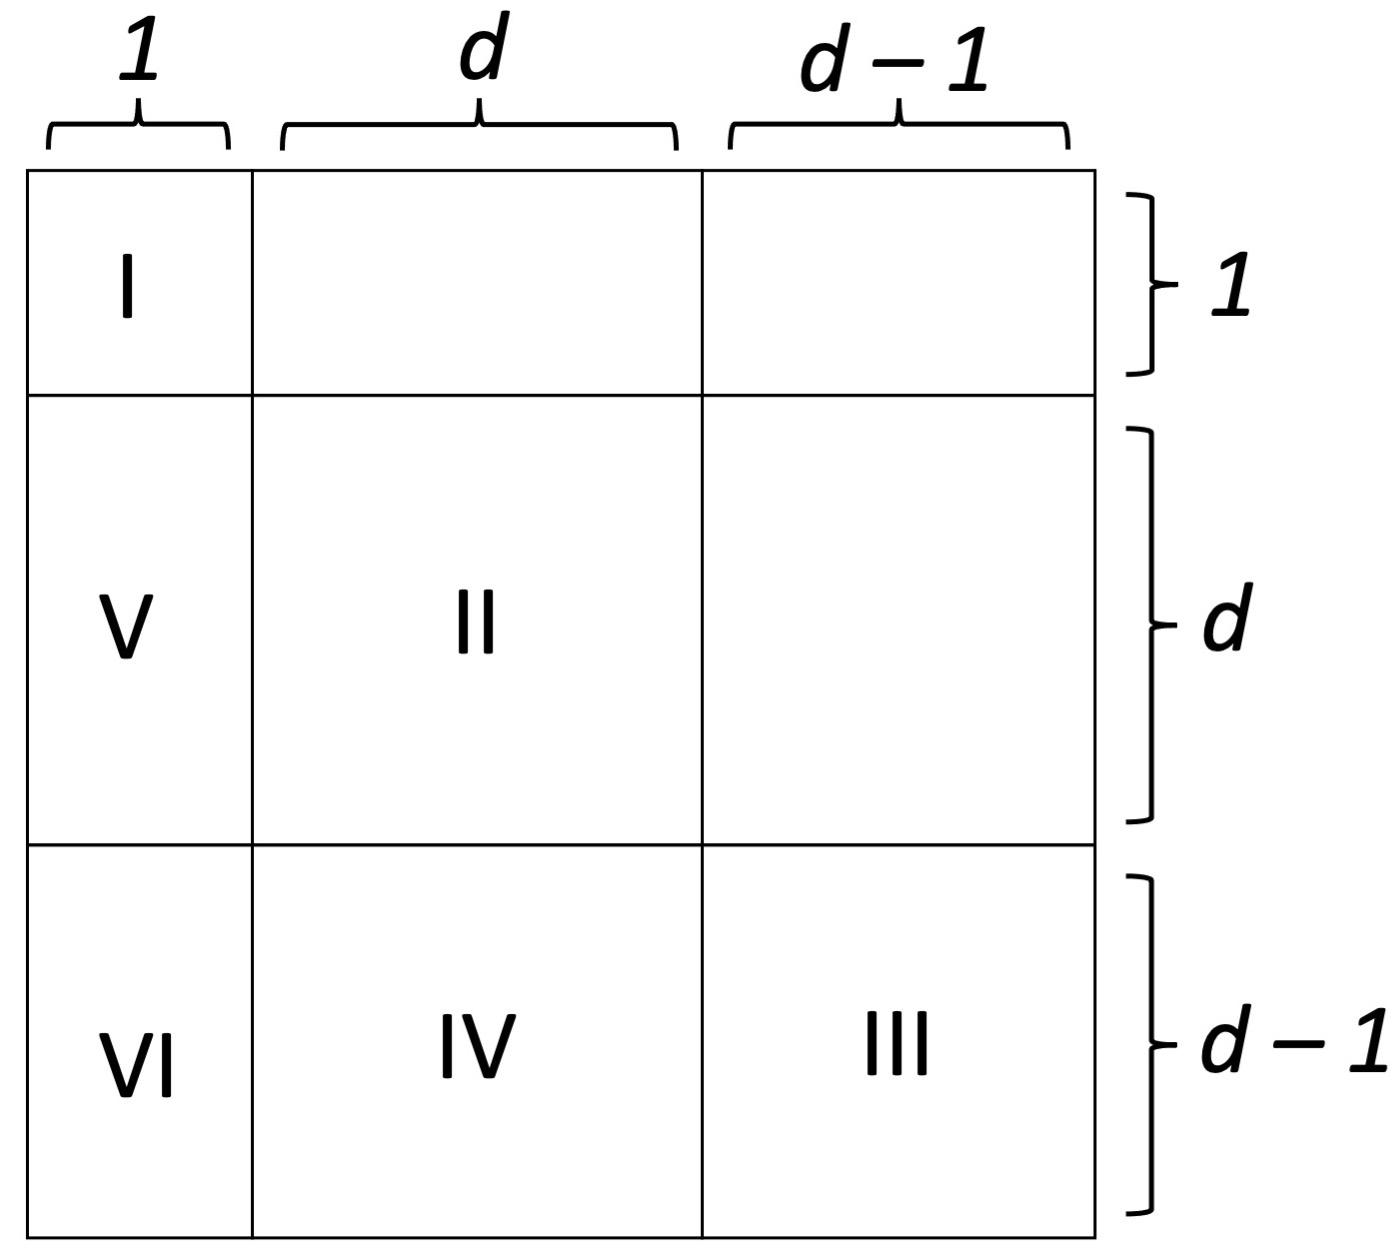
\includegraphics[width=0.45\linewidth]{../../figures/info_matrix/info_matrix_zero_inf}
	\caption{Block structure of the observed information matrix $J_z(\theta; m, g) = -\nabla^2 \mathcal{L}_z(\theta; m, g)$ for the zero-inflated model. Submatrices I, II, and VI are the same as in the background read model; therefore, we only need to compute submatrices III, VI, and V.}
	\label{infomatrixzeroinf}
\end{figure}

\subsubsection*{Submatrix III (zero-inflated)}
Denote submatrix III by $J_{\beta_{(g,z)}}(\theta; m, g)$ The formula for $J_{\beta_{(g,z)}}(\theta; m, g)$ is
\begin{multline}\label{sub_mat_3_zeroinf}
J_{\beta_{(g,z)}}(\theta; m, g) = -\E \left[\nabla_{\beta_{(g,z)}}^2 \mathcal{L}_z(\theta; m, g, p) \right] + \E\left[ \nabla_{\beta_{(g,z)}} \mathcal{L}_z(\theta; m, g, p) \right] \E\left[\nabla_{\beta_{(g,z)}} \mathcal{L}_z(\theta; m, g, p) \right]^T \\ - \E\left[ \nabla_{\beta_{(g,z)}} \mathcal{L}_z(\theta; m, g, p) \nabla_{\beta_{(g,z)}} \mathcal{L}_z(\theta; m, g, p)^T \right].
\end{multline}
GLM theory indicates that
$$ -\nabla_{\beta_{(g,z)}}^2 \mathcal{L}_z(\theta; m, g, p) =  X^T P ( \Delta^{(g,z)}V^{(g,z)}\Delta^{(g,z)} - (\Delta')^{(g,z)} H^{(g,z)}) X$$ and
$$ \nabla_{\beta_{(g,z)}} \mathcal{L}_z(\theta; m, g, p) = X^T P \Delta^{(g,z)} s^{(g,z)}.$$
We begin by computing the first term of (\ref{sub_mat_3_zeroinf}). The only random matrix among $X,$ $P$, $\Delta^{(g,z)}$, $V^{(g,z)}$, $(\Delta')^{(g,z)},$ and $H^{(g,z)}$ is $P$. Therefore, by the linearity of expectation,
\begin{multline}\label{sub_mat_3_zeroinf_1}
-\E \left[\nabla_{\beta_{(g,z)}}^2 \mathcal{L}_z(\theta; m, g, p) \right]   = \E \left[ X^T P (\Delta^{(g,z)}V^{(g,z)}\Delta^{(g,z)} - (\Delta')^{(g,z)} H^{(g,z)} \right] \\ = X^T T^{\theta}(1) ( \Delta^{(g,z)}V^{(g,z)}\Delta^{(g,z)} - (\Delta')^{(g,z)} H^{(g,z)}) X.
\end{multline}
Next, we compute the difference of the last two terms of (\ref{sub_mat_3_zeroinf}). The $(k,l)$th entry of this matrix is
\begin{multline*}
\bigg[ \E \left[\nabla_{\beta_{(g,z)}} \mathcal{L}_z(\theta; m, g, p) \right] \E \left[\nabla_{\beta{(g,z)}} \mathcal{L}_z(\theta; m, g, p)\right]^T \\ - \E \left[ \nabla_{{\beta_{(g,z)}}} \mathcal{L}_z(\theta; m, g, p) \nabla_{{\beta_{(g,z)}}} \mathcal{L}_z(\theta; m, g, p)^T \right] \bigg] [k,l] \\ 
= \left[ \E \left[ {X}^T P \Delta^{(g,z)} s^{(g,z)} \right]\E \left[ {X}^T P \Delta^{(g,z)} s^{(g,z)} \right]^T\right][k,l] - \E \left[ {X}^T P \Delta s^{(g,z)} (s^{(g,z)})^T \Delta^{(g,z)} P {X}^T \right][k,l] \\ 
= \E\left[{X}[,k]^T P \Delta^{(g,z)} s^{(g,z)} \right] \E \left[ {X}[,l]^T P \Delta^{(g,z)} s^{(g,z)} \right] - \E \left[ {X}[,k]^T P \Delta^{(g,z)} s^{(g,z)} (s^{(g,z)})^T \Delta^{(g,z)} P {X}[,l ] \right] \\
=\E\left(\sum_{i=1}^n {x}_{ik} P_i \Delta^{(g,z)}_i s^{(g,z)}_{i} \right) \E \left( \sum_{j=1}^n {x}_{jl} P_j \Delta^{(g,z)}_j s^{(g,z)}_j \right) \\ - \E \left( \sum_{i=1}^n \sum_{j=1}^n {x}_{ik} P_i \Delta^{(g,z)}_i s^{(g,z)}_i s^{(g,z)}_j \Delta^{(g,z)}_j P_j{x}_{jl} \right) \\ 
= \sum_{i=1}^n \sum_{j=1}^n \E[ {x}_{ik} P_i \Delta^{(g,z)}_is^{(g,z)}_i] \E [ {x}_{jl} P_j \Delta^{(g,z)}_j s^{(g,z)}_j]  -  \sum_{i=1}^n \sum_{j=1}^n \E [ {x}_{ik} P_i \Delta^{(g,z)}_i s^{(g,z)}_i s^{(g,z)}_j \Delta^{(g,z)}_jP_j {x}_{jl}  ]  \\
= \sum_{i=1}^n \sum_{j=1}^n \E[ {x}_{ik} P_i \Delta^{(g,z)}_i s^{(g,z)}_i ] \E \left[{x}_{jl} P_j \Delta^{(g,z)}_j s^{(g,z)}_j \right]  - \sum_{i \neq j} \E [{x}_{ik} P_i \Delta^{(g,z)}_i s^{(g,z)}_i] \E[s^{(g,z)}_j P_j \Delta^{(g,z)}_j {x}_{jl}] \\ - \sum_{i=1}^n \E[ {x}_{ik}P_i \Delta^{(g,z)}_i s^{(g,z)}_i s^{(g,z)}_i \Delta^{(g,z)}_i P_i{x}_{il}] \\ 
= \sum_{i=1}^n \E[ {x}_{ik} P_i \Delta^{(g,z)}_i H^{(g,z)}_i] \E[{x}_{il}P_i\Delta^{(g,z)}_i H^{(g,z)}_i] - \sum_{i=1}^n \E[{x}_{ik}P_i^2(\Delta^{(g,z)}_i)^2 (H^{(g,z)}_i)^2 {x}_{il}] \\ = \sum_{i=1}^n {x}_{ik} T_i^{\theta}(1)^2(\Delta^{(g,z)}_i)^2 (H_i^{(g,z)})^2{x}_{il} - \sum_{i=1}^n {x}_{ik} T_i^{\theta}(1) (\Delta_i^{(g,z)})^2 (H_i^{(g,z)})^2 {x}_{il} \\ = {X}[,k]^T T^{\theta}(1)^2 (\Delta^{(g,z)})^2 (H^{(g,z)})^2 {X}[,l] - {X}[,k]^T T^{\theta}(1) (\Delta^{(g,z)})^2 (H^{(g,z)})^2 {X}[,l]
\end{multline*}
Therefore, we have that
\begin{multline}\label{sub_mat_3_zeroinf_2}
\E\left[ \nabla_{\beta_{(g,z)}} \mathcal{L}_z(\theta; m, g, p) \right] \E\left[\nabla_{\beta_{(g,z)}} \mathcal{L}_z(\theta; m, g, p) \right]^T - \E\left[ \nabla_{\beta_{(g,z)}} \mathcal{L}_z(\theta; m, g, p) \nabla_{\beta_{(g,z)}} \mathcal{L}_z(\theta; m, g, p)^T \right] \\ = 
X^T T^{\theta}(1)^2 (\Delta^{(g,z)})^2(H^{(g,z)})^2{X} - {X}^T T^{\theta}(1) (\Delta^{(g,z)})^2 (H^{(g,z)})^2 {X} \\ = - X^T T^{\theta}(1) \left(\Delta^{(g,z)}\right)^2 \left( H^{(g,z)} \right)^2 \left( I - T^{\theta}(1)  \right) X.
\end{multline}
Combining (\ref{sub_mat_3_zeroinf}), (\ref{sub_mat_3_zeroinf_1}), and (\ref{sub_mat_3_zeroinf_2}), we conclude that
\begin{multline}\label{sub_mat_3_zeroinf_formula}
J_{\beta_{(g, z)}} = \left( \theta; m, g \right) =  X^T T^{\theta}(1) ( \Delta^{(g,z)}V^{(g,z)}\Delta^{(g,z)} - (\Delta')^{(g,z)} H^{(g,z)}) X \\ - X^T T^{\theta}(1) \left(\Delta^{(g,z)}\right)^2 \left( H^{(g,z)} \right)^2 \left( I - T^{\theta}(1) \right) X.
\end{multline}

\subsubsection*{Submatrix IV (zero-inflated)}
Denote submatrix IV by $J_{(\beta_{(g,z)}, \beta_m)}(\theta; m, g)$. The formula for submatrix IV is
\begin{multline}\label{sub_mat_4_zeroinf}
J_{(\beta_{(g,z)}, \beta_m)}(\theta; m, g) = - \E \left[\nabla_{\beta_{(g,z)}} \nabla_{\beta_m} \mathcal{L}_z (\theta; m, g, p) \right] \\ + \E\left[ \nabla_{\beta_{(g,z)} }\mathcal{L}_z(\theta ; m,g,p) \right]\E\left[\nabla_{\beta_m}\mathcal{L}_z(\theta; m,g,p)\right]^T - \E \left[\nabla_{\beta_{(g,z)}}\mathcal{L}_z (\theta; m,g,p) \nabla_{\beta_m}\mathcal{L}_z(\theta; m,g,p)]^T \right].
\end{multline} 
First, we have that
\begin{equation}\label{sub_mat_4_zeroinf_1}
- \E \left[\nabla_{\beta_{(g,z)}} \nabla_{\beta_m} \mathcal{L}_z (\theta; m, g, p) \right] = 0,
\end{equation}
 as the derivative in $\beta_m$ of $\mathcal{L}_z(\theta; m, g, p)$ is a function of $\beta_m$, and the derivative in $\beta_{(g,z)}$ of this term is $0$. Next, we compute the difference of the last two terms of (\ref{sub_mat_4_zeroinf}). Entry $(k,l)$ of this matrix is
\begin{multline}\label{sub_mat_4_zeroinf_2}
[\E[\nabla_{\beta_{(g,z)}}\mathcal{L}_z(\theta; m, g, p) ] \E [\nabla_{\beta_m} \mathcal{L}_z(\theta; m, g, p) ]^T \\ - \E [\nabla_{\beta_{(g,z)}} \mathcal{L}_z(\theta; m, g, p) \nabla_{\beta_m}\mathcal{L}_z(\theta; m, g, p)^T ] ][k,l] \\ 
= \left[ \E \left[ {X}^T P \Delta^{(g,z)} s^{(g,z)} \right] \E\left[\tilde{X}^T \Delta^m s^m\right]^T\right][k,l] - \E \left[{X}^T P \Delta^{(g,z)} s^{(g,z)} (s^m)^T \Delta^m \tilde{X} \right][k,l] \\ = \left[\E\left[{X}[,k]^T P \Delta^{(g,z)} s^{(g,z)}\right]\E\left[\tilde{X}[,l]^T \Delta^m s^m\right]^T\right] - \E \left[{X}[,k]^T P \Delta^{(g,z)} s^{(g,z)} (s^m)^T \Delta^m \tilde{X}[,l] \right] \\ = \E\left(\sum_{i=1}^n x_{ik} P_i \Delta^{(g,z)}_i s^{(g,z)}_i\right) \E \left(\sum_{j=1}^n \tilde{x}_{jl} \Delta^m_j s^m_j \right) - \E \left(\sum_{i=1}^n \sum_{j=1}^n x_{ik} P_i \Delta^{(g,z)}_i s^{(g,z)}_i \Delta^m_j s^m_j \tilde{x}_{jl}  \right) \\ 
= \sum_{i=1}^n \sum_{j=1}^n \E [x_{ik} P_i \Delta^{(g,z)}_i s^{(g,z)}_i] \E[\Delta^m_js^m_j \tilde{x}_{jl}] - \sum_{i=1}^n \sum_{j=1}^n \E[x_{ik} P_i \Delta^{(g,z)}_i s^{(g,z)}_i \Delta^m_j s^m_j \tilde{x}_{jl}] \\
= \sum_{i=1}^n \sum_{j=1}^n \E [x_{ik} P_i \Delta^{(g,z)}_i s^{(g,z)}_i ] \E[\Delta^m_js^m_j \tilde{x}_{jl}] - \sum_{i \neq j} \E [x_{ik} P_i \Delta^{(g,z)}_i s^{(g,z)}_i] \E[\Delta^m_js^m_j \tilde{x}_{jl}] \\ - \sum_{i=1}^n \E[x_{ik} P_i \Delta^{(g,z)}_i s^{(g,z)}_i \Delta^m_j s^m_j \tilde{x}_{jl}] \\
= \sum_{i=1}^n \E[x_{ik} P_i \Delta_i^{(g,z)} H^{(g,z)}_i] \E[\tilde{x}_{il} \Delta^m_i H^m_i] - \sum_{i=1}^n \E[x_{ik} P_i \Delta_i^{(g,z)} H_i^{(g,z)} \Delta_i^m H_i^m \tilde{x}_{il}] \\ 
= \sum_{i=1}^n \left[x_{ik} T_i^\theta(1) \Delta^{(g,z)}_i H^{(g,z)}_i \right] \cdot \left[{\Delta}^m_i(0) T^\theta_i(0) {H}^m_i(0) \tilde{x}_{il}(0) + {\Delta}^m_i(1) T_i^\theta(1) {H}^m_i(1) \tilde{x}_{il}(1)\right]
\\ - \sum_{i=1}^n \left[x_{ik} T_i^\theta(1) \Delta^{(g,z)}_i H^{(g,z)}_i \Delta^m_i(1) H^m_i(1) \tilde{x}_{il}(1)\right] 
\\ = \sum_{s=0}^1 \sum_{i=1}^n x_{ik} T_i^\theta(1) H_i^{(g,z)} \Delta_i^{(g,z)} T^\theta_i(s) \Delta_i^m(s) H^m(s) \tilde{x}_{il}(s) \\ - \sum_{i=1}^n \left[x_{il}T_i^\theta(1) \Delta^{(g,z)}_i H^{(g,z)}_i \Delta^m_i(1) H^m_i(1) \tilde{x}_{ik}(1)\right] \\ = \sum_{s=0}^1 X[,k]^T T^\theta(1) H^{(g,z)} \Delta^{(g,z)} T^\theta(s)\Delta^m(s)H^m(s) \tilde{X}(s)[,l] \\ - X[,k]^T \Delta^{(g,z)} H^{(g,z)} T^\theta(1)\Delta^m(1) H^m(1) \tilde{X}[,l].
\end{multline}
Combining (\ref{sub_mat_3_zeroinf}), (\ref{sub_mat_3_zeroinf_1}), and (\ref{sub_mat_3_zeroinf_2}) yields
\begin{multline}\label{sub_mat_4_zeroinf_formula} J_{(\beta_{(g,z)}, \beta_m)}(\theta; m, g) = \left(\sum_{s=0}^1 X^T  T^\theta(1) H^{(g,z)} \Delta^{(g,z)} T^\theta(s) \Delta^m(s) H^m(s) \tilde{X}(s) \right) \\ - X^T \Delta^{(g,z)} H^{(g,z)} T^\theta(1) \Delta^m(1)H^m(1) \tilde{X}(1).
\end{multline}

\subsubsection*{Submatrix VI (zero-inflated)}
Denote submatrix VI by $J_{(\beta_{(g,z)},\pi)}(\theta; m, g).$ The formula for $J_{(\beta_{(g,z)},\pi)}(\theta; m, g)$ is
\begin{multline}\label{sub_mat_6_zeroinf}
J_{(\beta_{(g,z)},\pi)}(\theta; m, g) = \E \left[-\nabla_{\beta_{(g,z)}} \nabla_{\pi} \mathcal{L}_z(\theta; m, g, p) \right] + \E\left[ \nabla_{\beta_{(g,z)}}\mathcal{L}_z(\theta; m, g ,p)\right] \E \left[ \nabla_{\pi}\mathcal{L}_z(\theta; m,g,p) \right] \\ - \E \left[ \nabla_{\beta_{(g,z)}}\mathcal{L}_z(\theta; m,g,p) \nabla_{\pi}\mathcal{L}_z(\theta; m,g,p) \right].
\end{multline} Recall that $\nabla_{\beta_{(g,z)}} \mathcal{L}_z(\theta; m, g, p) = X^T P \Delta^{(g,z)}s^{(g,z)}$ and $\nabla_\pi \mathcal{L}_z(\theta; m, g, p) = a \left(\sum_{i=1}^n p_i\right) - b,$ where $$a = \frac{1}{\pi} + \frac{1}{1 - \pi}, \textrm{    } b = \frac{n}{1 - \pi}.$$ 
We have that
\begin{equation}\label{sub_mat_6_zeroinf_1}
\E \left[-\nabla_{\beta_{(g,z)}} \nabla_{\pi} \mathcal{L}_z(\theta; m, g, p) \right] = 0,
\end{equation}
as the derivative in $\pi$ of $\mathcal{L}_z(\theta; m, g, p)$ is a function of $\pi$, and the derivative in $\beta_{(g,z)}$ of this term is $0$. Next, we compute the difference of the second two terms of (\ref{sub_mat_6_zeroinf}). The $k$th entry of this vector is
\begin{multline}\label{sub_mat_6_zeroinf_2}
\E \left[ \nabla_\pi \mathcal{L}_z(\theta; m, g, p) \right] \E\left[\nabla_{\beta_{(g,z)}} \mathcal{L}_z(\theta; m, g, x)[k] \right] - \E \left[\nabla_{\pi}\mathcal{L}(\theta; m,g,p) \nabla_{\beta_{(g,z)}} \mathcal{L} (\theta; m,g,p)[k] \right] \\= \left(\E \left[ a \sum_{i=1}^n p_i - b \right] \right)\left( \E \left[{X}[,k]^T P \Delta^{(g,z)} s^{(g,z)} \right]\right) - \E \left[ \left( a \sum_{i=1}^n p_i - b \right) {X}[,k]^T P \Delta^{(g,z)} s^{(g,z)}\right] \\ = \left( a \sum_{i=1}^n \E[p_i] - b \right) \left( \sum_{j=1}^n \E [x_{jk} p_j \Delta^{(g,z)}_j s^{(g,z)}_j] \right) \\ - \E \left[ \left( a \sum_{i=1}^n p_i - b \right) \left( \sum_{j=1}^n \tilde{x}_{jk} p_j \Delta^{(g,z)}_j s^{(g,z)}_j \right) \right] \\= a \sum_{i=1}^n \sum_{j=1}^n \E [p_i] \E[x_{jk} p_j \Delta^{(g,z)}_j s^{(g,z)}_j] - b \sum_{j=1}^n \E[x_{jk} p_j \Delta^{(g,z)}_j s^{(g,z)}_j] \\ - \left[a \sum_{i=1}^n \sum_{j=1}^n \E [ p_i x_{jk} p_j \Delta^{(g,z)}_j s^{(g,z)}_j] - b \sum_{j=1}^n \E[x_{jk} p_j \Delta^{(g,z)}_j s^{(g,z)}_j] \right] \\ = a \sum_{i=1}^n \sum_{j=1}^n \E[p_i] \E[{x}_{jk} p_j \Delta^{(g,z)}_j s^{(g,z)}_j] - a \sum_{i \neq j} \E[p_i] \E[x_{jk} p_j \Delta^{(g,z)}_j s^{(g,z)}_j] - a \sum_{i=1}^n \E[ x_{ik} p_i^2 \Delta^{(g,z)}_i s^{(g,z)}_i] \\ = a \sum_{i=1}^n \E[p_i] \E[x_{ik} p_i \Delta^{(g,z)}_i s^{(g,z)}_i] - a \sum_{i=1}^n \E[x_{ik} p_i^2 \Delta^{(g,z)}_i s^{(g,z)}_i] \\ = a \sum_{i=1}^n T^\theta_i(1) x_{ik} T^\theta_i(1) \Delta^{(g,z)}_i s^{(g,z)}_i - a \sum_{i=1}^n x_{ik} T^\theta_i(1) \Delta^{(g,z)}_i s^{(g,z)}_i \\ = a \sum_{i=1}^n \left( {x}_{ik} T^\theta_i(1)^2 \Delta^{(g,z)}_i s^{(g,z)}_i - x_{ik} T^\theta_i(1) \Delta^{(g,z)}_i s^{(g,z)}_i \right) = a \sum_{i=1}^n {x}_{ik}T^\theta_i(1)\Delta^{(g,z)}_i s^{(g,z)}_i \left( T^\theta_i(1) - 1\right) \\ = -a\sum_{i=1}^n x_{ik} T_i(0) T^\theta_i(1)\Delta^{(g,z)}_i H^{(g,z)}_i = -a X[,k]^T w^{(g,z)}.
\end{multline}
Combining (\ref{sub_mat_6_zeroinf}), (\ref{sub_mat_6_zeroinf_1}), and (\ref{sub_mat_6_zeroinf_2}), we conclude that
\begin{equation}\label{sub_mat_6_zeroinf_formula} J_{(\beta_{(g,z)},\pi)}(\theta; m, g) = -\left( \frac{1}{\pi} + \frac{1}{1-\pi} \right)X^T w^{(g,z)}.\end{equation}

\section{Statistical accelerations}\label{sec:statistical_accelerations}

\subsection*{Computing $\pi^\textrm{pilot}$, $[\beta^m_1]^\textrm{pilot}$, $[\beta^m_1]^\textrm{pilot}$}

We present the algorithm (Algorithm \ref{algo:pilot_estimates_2}) for computing the pilot estimates $\pi^\textrm{pilot}$, $[\beta^m_1]^\textrm{pilot}$, $[\beta^m_1]^\textrm{pilot}$. This algorithm, alongside Algorithm \ref{algo:pilot_estimates_1}, is used to compute pilot estimates for use in Algorithm \ref{algo:em_full}.

\begin{algorithm}
	\caption{Computing $\pi^\textrm{pilot}$, $[\beta^m_1]^\textrm{pilot}$, $[\beta^m_1]^\textrm{pilot}$.}\label{algo:pilot_estimates_2}
	\begin{algorithmic}[2]
		\Require Data $m$, $g$; fitted offsets $\hat{f}^m,$ $\hat{f}^g$.
		\State \texttt{bestLik} $\gets -\infty$ \Comment{Reduced GLM-EIV}
		\For{$i \in \{1,\dots,B\}$}
		\State Randomly generate starting parameters $\pi^\textrm{curr}, [\beta_1^m]^\textrm{curr}, [\beta^g_1]^\textrm{curr}.$
		\While{Not converged}
		\For{$i \in \{1, \dots, n\}$} \Comment{E step}
		\State $T_i(1) \gets \P(P_i = 1 | M_i = m_i, G_i = g_i, \pi^\textrm{curr}, [\beta^g_1]^\textrm{curr}, [\beta_1^m]^\textrm{curr})$
		\State $T_i(0) \gets 1 - T_i(1)$
		\EndFor
		\State $\pi^{\textrm{curr}} \gets (1/n) \sum_{i=1}^n T_i(1)$ \Comment{M step}
		\State $w \gets [T_1(0), T_2(0), \dots, T_n(0), T_1(1), T_2(1), \dots, T_n(1)]^T$
		\For{$k \in \{g,m\}$}
		\State \multiline{Fit no-intercept, univariate GLM $GLM_k$ with predictors $[\underbrace{0, \dots, 0}_\textrm{n}, \underbrace{1, \dots, 1}_\textrm{n}]$, responses $[k,k]^T$, offsets $[\hat{f}^k, \hat{f}^k]^T,$ and weights $w$.}
		\State Set $[\beta^k_1]^\textrm{curr}$ to fitted coefficient of $GLM_k$.
		\EndFor
		\State \multiline{
			Compute log likelihood \texttt{currLik} using $\pi^\textrm{curr}$,$ [\beta^m_1]^\textrm{curr}$, and $[\beta^g_1]^\textrm{curr}.$}
		\EndWhile
		\If{\texttt{currLik} $>$ \texttt{bestLik}}
		\State bestLik $\gets$ currLik
		\State $\pi^\textrm{pilot} \gets \pi^\textrm{curr};$ $[\beta^m_1]^\textrm{pilot} \gets [\beta^m_1]^\textrm{curr}; [\beta^g_1]^\textrm{pilot} \gets [\beta^g_1]^\textrm{curr}$
		\EndIf
		\EndFor
		\State \textbf{return} $(\pi^\textrm{pilot}, [\beta^m_1]^\textrm{pilot}, [\beta^g_1]^\textrm{pilot})$
	\end{algorithmic}
\end{algorithm}

\subsection*{Intercept-plus-offset models}

A key step in the algorithm for computing the pilot parameter estimates (Algorithm \ref{algo:pilot_estimates_2}) is to fit a weighted, no-intercept, univariate GLM with nonzero offset terms and a binary predictor variable. We derive an analytic formula for the MLE of this GLM for three important pairs of response distributions and link functions: Gaussian response with identity link, Poisson response with log link, and negative binomial response with log link. The GLM that we seek to estimate has responses $[m,m]^T$, predictors $[\underbrace{0, \dots, 0}_\textrm{n}, \underbrace{1, \dots, 1}_\textrm{n}]$, offsets $[\hat{f}^m, \hat{f}^m],$ and weights $w = [T_1(0), \dots, T_n(0), T_1(1), \dots, T_n(1)]^T.$ Throughout, $C$ denotes a universal constant. The log likelihood of this GLM is
\begin{multline}\label{stat_acc_1}
$$\mathcal{L}(\beta_1; m) = \sum_{i=1}^n T_i(0) f_m(m_i; h_m(\beta_1 + \hat{f}^m_i )) + \sum_{i=1}^n T_i(1) f_m(m_i; h_m(\hat{f}^m_i)) \\ = \sum_{i=1}^n T_i(1) f_m(m_i; h_m(\beta_1 + \hat{f}^m_i )) + C.$$
\end{multline}
Thus, finding the MLE $\hat{\beta_1}$ is equivalent to estimating a GLM with intercept $\beta_1$, offsets $\hat{f}^m$, weights $T_i(1)$, and \textit{no} covariate terms. We term such a GLM a \textit{intercept-plus-offset} model. Below, we study intercept-plus-offset models in generality.

Let $\beta \in \R$ be an unknown constant. Let $o_1, \dots, o_n \sim \mathcal{P}_1$, where $\mathcal{P}_1$ is a distribution. Let $Y_i|o_i, \dots, Y_n|o_i$ be exponential family-distributed random variables with identity sufficient statistic. Suppose the mean $\mu_i$ of $Y_i|o_i$ is given by $r(\mu_i) = \beta + o_i,$ where $r: \R \to \R$ is a strictly increasing, differentiable link function. We call this model the \textit{intercept-plus-offset} model.

We derive the (weighted) log likelihood of this model. Let $w_1, \dots, w_n \sim \mathcal{P}_2$ be weights, where $\mathcal{P}_2$ is a distribution bounded above by $1$ and below by $0$. (A special case, which corresponds to no weights, is $w_i = 1$ for all $i \in \{1, \dots, n\}$.) Throughout, we assume that $y_iw_i$ and $\exp(o_i)w_i$ have finite first moment.  Suppose the cumulant-generating function and carrying density of the exponential family distribution are $\psi:\R \to \R$ and $c: \R \to \R$, respectively. The canonical parameter $\eta_i$ of the $i$th observation is 
\begin{equation}\label{can_param}
\eta_i = ([\psi']^{-1} \circ r^{-1})(\beta + o_i) := h(\beta + o_i),
\end{equation}
 and the density $f$ of $Y_i | \eta_i$ is
$f(y_i; \eta_i) = \exp\{y_i \eta_i - \psi(\eta_i) + c(y_i)\}.$ The weighted log likelihood is
\begin{equation}\label{m_plus_o_mle}
\mathcal{L}(\beta;y_i) = \sum_{i=1}^n w_i\log\left[f(y_i;\eta_i)\right] = C + \sum_{i=1}^n w_i(y_i \eta _i - \psi(\eta_i)).
\end{equation}
Our goal is to find the weighted MLE $\hat{\beta}$ of $\beta$. We consider three important choices for the exponential family distribution and link function. % This amounts to maximizing (\ref{m_plus_o_mle}) for three specific choices of $r$ and $\psi$.
In the first two cases -- Gaussian distribution with identity link and Poisson distribution with log link -- we find the \textit{finite-sample} maximizer of (\ref{m_plus_o_mle}); by contrast, in the third case -- negative binomial distribution with log link -- we find an \textit{asymptotically exact} maximizer.

\subsubsection*{Gaussian}
First, consider a Gaussian response distribution and identity link function $r(\mu) = \mu$. The cumulant-generating function $\psi$ is $\psi(\eta) = \eta^2/2$, and so, by (\ref{can_param}),
$$h(t) = [\psi']^{-1}( r^{-1}(t)) = [\psi']^{-1}(t) = t.$$
Plugging $\eta_i = h(\beta + o_i) = \beta + o_i$ and $\psi(\eta_i) = (1/2)(\beta + o_i)^2$ into (\ref{m_plus_o_mle}), we obtain
$$\mathcal{L}(\beta; y) = \sum_{i=1}^n w_i (y_i(\beta + o_i) - (\beta + o_i)^2/2).$$ The derivative of this expression in $\beta$ is
$$\frac{\partial \mathcal{L}(\beta;y)}{\partial\beta} = \sum_{i=1}^n w_i (y_i - \beta - o_i) = \sum_{i=1}^n w_i(y_i - o_i) - \beta \sum_{i=1}^n w_i.$$ Setting this quantity to 0 and solving for $\beta$, we find that the MLE $\hat{\beta}^\textrm{gauss}$ is
$$\hat{\beta}^\textrm{gauss} = \frac{\sum_{i=1}^n w_i (y_i - o_i)}{\sum_{i=1}^n w_i}.$$

\subsubsection*{Poisson}
Next, consider a Poisson response distribution and log link function $r(\mu) = \log(\mu).$ The cumulant-generating function $\psi$ is $\psi(\eta) = e^\eta.$ Therefore, by (\ref{can_param}),
$$h(t) = [\psi']^{-1}(r^{-1}(t)) = [\psi']^{-1} \left(\exp(t) \right) = \log(\exp(t)) = t.$$ Plugging $\eta_i = h(\beta + o_i) = \beta + o_i$ and $\psi(\eta_i) = \exp(\beta + o_i)$ into (\ref{m_plus_o_mle}), we obtain
$$ \mathcal{L}(\beta; y) = \sum_{i=1}^n w_i \left( y_i(\beta + o_i) - \exp(\beta + o_i) \right).$$ The derivative of this function in $\beta$ is 
$$\frac{\partial \mathcal{L}(\beta; y)}{\partial \beta} = \sum_{i=1}^n w_iy_i - w_i \exp(\beta + o_i) = \sum_{i=1}^n w_i y_i - \exp(\beta) \sum_{i=1}^n w_i \exp(o_i).$$
Setting to zero and solving for $\beta$, we find that the MLE $\hat{\beta}^\textrm{pois}$ is
\begin{equation}\label{pois_mle}
\hat{\beta}^\textrm{pois} = \log\left(\frac{\sum_{i=1}^n w_i y_i}{\sum_{i=1}^n w_i e^{o_i}}\right).
\end{equation}

\subsubsection*{Negative binomial}
Finally, we consider a negative binomial response distribution (with fixed size parameter $\theta > 0$) and log link function $r(\mu) = \log(\mu)$. The cumulant-generating function $\psi$ is
$\psi(\eta) = -\theta \log(1 - e^\eta).$ The derivative $\psi'$ of $\psi$ is
$$ \psi'(t) = \theta \left(\frac{e^t}{1 - e^t}\right) = \frac{\theta}{e^{-t} - 1}.$$ Define the function $\delta: \R \to \R$ by $\delta(t) = -\log\left(\theta/t + 1 \right).$ We see that
$$\psi'(\delta(t)) = \frac{\theta}{\exp\left(\log(\theta/t + 1 )\right) - 1} = t,$$ implying $\delta = [\psi']^{-1}.$ By (\ref{can_param}), we have that
$$
h(t) = [\psi']^{-1}(r^{-1}(t)) = -\log\left(\frac{\theta}{\exp(t)} + 1 \right) = \log\left(\frac{\exp(t)}{\theta + \exp(t)}\right).
$$
Therefore,
\begin{equation}\label{nb_mo_1}
\eta_i = h(\beta + o_i) = \log\left(\frac{\exp(\beta+o_i)}{\theta + \exp(\beta + o_i)} \right) = \beta + o_i - \log\left(\theta + e^{\beta}e^{o_i}\right) = \beta - \log\left(\theta + e^{\beta}e^{o_i} \right) + C,
\end{equation}
 and
 \begin{multline}\label{nb_mo_2}
 \psi(\eta_i) = -\theta\log\left(1 - \frac{\exp(\beta+o_i)}{\theta + \exp(\beta + o_i)} \right) = -\theta \log \left(\frac{\theta}{\theta + \exp(\beta + o_i)} \right) \\ = -\theta \log (\theta) + \theta \log[\theta + \exp(\beta + o_i)] = \theta \log(\theta + e^{\beta}e^{o_i}) + C.
 \end{multline}
 Plugging (\ref{nb_mo_1}) and (\ref{nb_mo_2}) into (\ref{m_plus_o_mle}), the log-likelihood (up to a constant) is
\begin{multline*}
\mathcal{L}(\beta; y) = \beta \sum_{i=1}^n w_i y_i - \sum_{i=1}^n w_i y_i \log(\theta + e^\beta e^{o_i}) - \theta \sum_{i=1}^n w_i \log(\theta + e^\beta  e^{o_i}) \\ = \beta \sum_{i=1}^n w_i y_i - \sum_{i=1}^n (y_i + \theta)w_i\log(\theta + e^\beta e^{o_i}).
\end{multline*}
The derivative of $\mathcal{L}$ in $\beta$ is
$$\frac{\partial \mathcal{L}(\beta;y)}{\partial \beta} = \sum_{i=1}^n w_i y_i  - \sum_{i=1}^n \frac{w_i(y_i + \theta) e^{\beta} e^{o_i}}{ \theta + e^{\beta} e^{o_i}}.$$
Setting the derivative to zero, the equation defining the MLE is
\begin{equation}\label{nb_mle}
e^\beta \sum_{i=1}^n \frac{w_i e^{o_i} (y_i + \theta)}{e^\beta e^{o_i} + \theta} = \sum_{i=1}^n w_i y_i.
\end{equation}
We cannot solve for $\beta$ in (\ref{nb_mle}) analytically. However, we can derive an asymptotically exact solution. By the law of total expectation,
$$ \E \left[\frac{w_i  e^{o_i} (y_i + \theta)}{e^{\beta + o_i} + \theta} \right] = \E \left[\E\left[\frac{w_i e^{o_i} (y_i + \theta) }{e^{\beta + o_i} + \theta} \bigg| (o_i, w_i) \right] \right] = \E \left[\frac{w_i e^{o_i} (e^{\beta + o_i} + \theta)}{ e^{\beta + o_i} + \theta} \right] = \E [w_i e^{o_i}];
$$
the second equality holds because $\E[y_i | o_i ] = \mu_i = e^{\beta + o_i}.$ Dividing by $n$ on both sides of (\ref{nb_mle}) and rearranging,
\begin{equation}\label{nb_mo_3}
\beta = \log\left( \frac{ (1/n) \sum_{i=1}^n w_i e^{o_i} (y_i + \theta)/(e^\beta e^{o_i} + \theta)}{ (1/n) \sum_{i=1}^n w_i y_i. } \right).
\end{equation}
By weak LLN, the limit (in probability) of the MLE $\hat{\beta}^\textrm{NB}$ is
\begin{equation}
\hat{\beta}^{\textrm{NB}} \xrightarrow{P} \log\left(\frac{\E[w_i y_i]}{\E[w_i e^{o_i}]} \right).
\end{equation}
But the Poisson MLE $\hat{\beta}^{\textrm{Pois}}$ (\ref{pois_mle}) converges in probability to the same limit:
$$ \hat{\beta}^{\textrm{pois}} =  \log \left(\frac{ (1/n) \sum_{i=1}^n w_i y_i}{(1/n)\sum_{i=1}^n w_i e^{o_i}} \right) \xrightarrow{P} \log \left(\frac{\E[w_i y_i]}{ \E[w_i e^{o_i}]} \right).$$ Therefore, for large $n$, we can approximate $\hat{\beta}^{\textrm{NB}}$ by $\hat{\beta}^{\textrm{pois}}$.

Suppose the log likelihood is unweighted (i.e., $w_i = 1$ for all $i$). We present an alternate (and simpler, more general) derivation of the approximate formula for the MLE. Let $y_i$ be a random variable with finite first moment and conditional mean $\E[y_i | o_i] = \exp(\beta + o_i).$ By the law of total expectation,
$$ \E[y_i] = \E[\E[ y_i | o_i]] = \E[\exp(\beta + o_i)] = \exp(\beta) \E(e^{o_i}),$$ or
\begin{equation}\label{nb_mo_4}
\beta = \log\left(\frac{\E[y_i]}{E[e^{o_i}]} \right).
\end{equation}
Assuming the MLE is well-behaved, we have that $\hat{\beta} \xrightarrow{P} \beta.$ On the other hand, by WLLN and (\ref{nb_mo_4}),
\begin{equation}\label{nb_mo_5}
\log\left( \frac{(1/n) \sum_{i=1}^n y_i }{(1/n) \sum_{i=1}^n e^{o_i}} \right) \xrightarrow{P}  \log\left(\frac{ \E[y_i] }{ \E[e^{o_i}] } \right) = \beta.
\end{equation}
 Therefore, the LHS of (\ref{nb_mo_5}) approximates the MLE $\hat{\beta}$ for large $n$.

\subsection*{Application to GLM-EIV}
The GLM that we seek to estimate (\ref{stat_acc_1}) is an approximate intercept-plus-offset model: $T_1(1), \dots, T_n(1)$ are the weights $w_1,\dots, w_n$, and $\hat{f}^m_1, \dots, \hat{f}^m_n$ are the offsets $o_1, \dots, o_m$. Of course, $T_1(1), \dots, T_1(n)$ are in general dependent random variables, as are $\hat{f}^m_1, \dots, \hat{f}^m_n.$ $T_i(1)$ depends on $m_i$ and $g_i$, as well as the final parameter estimate $(\hat{\pi}, \hat{\beta}_m, \hat{\beta}_g),$ which itself is a function of $m$ and $g$; the situation is similar for the $\hat{f}^m_i$s. In practice, we find that the intercept-plus-offset model is very good approximation to the GLM (\ref{stat_acc_1}), especially when the number of cells $n$ is large. Additionally, we note that the GLM (\ref{stat_acc_1}) is fit as a subroutine of the algorithm for producing pilot parameter estimates (Algorithm \ref{algo:pilot_estimates}). The quality of the pilot parameter estimates does not affect the validity of the estimation and inference procedures (Algorithm \ref{algo:em_full}), barring issues related to convergence to local optima (which are outside the scope fo the current work).

\section{Additional simulation study}\label{sec:extra_sims}
We ran an additional simulation study in which we modeled the gene and gRNA expressions using a Gaussian distribution with identity link. We generated data on $n = 150,000$ cells, fixing the target of inference $\beta^m_1$ to $-4$ and the probability of perturbation $\pi$ to $0.05$. We included ``sequencing batch'' (modeled as a Bernoulli-distributed variable) and ``sequencing depth'' (modeled as a Poisson-distributed variable) as covariates in the model. We did not include sequencing depth as an offset because use of the identity link renders offsets meaningless. We varied $\beta^g_1$ over a grid on the interval $[0,7].$ We generated $n_\textrm{sim} = 1,000$ synthetic datasets for each value of $\beta^g_1$. We applied accelerated GLM-EIV and thresholded regression to the simulated data. We assessed these methods on the metrics of bias, mean squared error, confidence interval coverage rate, and confidence interval width. We found that accelerated GLM-EIV outperformed the thresholding method: the former method exhibited smaller bias, smaller mean squared error, higher confidence interval coverage rate, and smaller confidence interval width than the latter method (Figure \ref{fig:gaussian_sim}). 

\begin{figure}
	\centering
	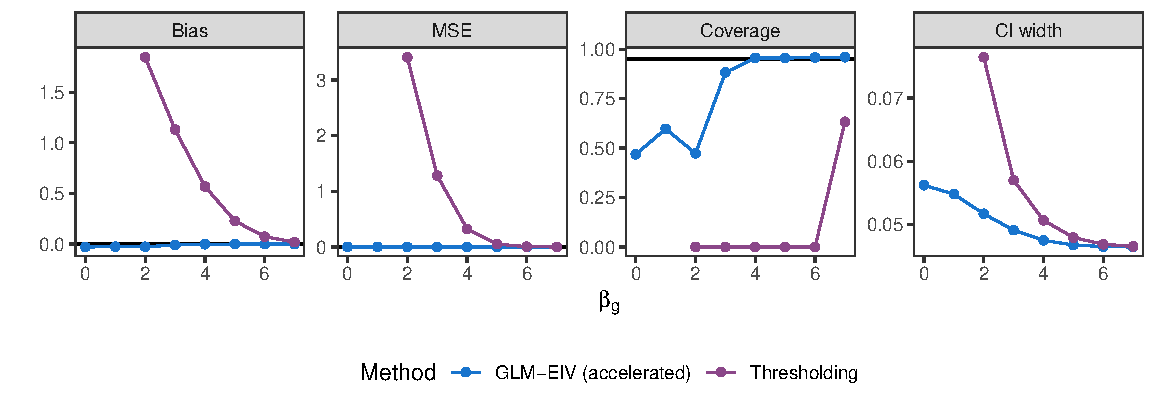
\includegraphics[width=1.0\linewidth]{../../figures/supplement_sim/gaussian}
	\caption{Additional simulation results on Gaussian data. GLM-EIV (accelerated) outperformed the thresholding method on bias, mean squared error, confidence interval coverage rate, and confidence interval width metrics.}\label{fig:gaussian_sim}
\end{figure}

\section{Data analysis details}\label{sec:data_analysis_details}

We performed quality control. We kept cells with percent mitochondrial reads less than 8$\%$. For the Gasperini dataset, we furthermore kept cells with UMI and gRNA counts in the 5th to 95th percentiles to reduce the effect of outliers. (We did not perform this latter filter on the Xie data, as the latter dataset appeared to be less noisy and contained fewer cells.) Next, we kept genes expressed in at least $10\%$ of cells with a mean expression level of at least $1$. We did not QC the gRNAs.

The quality-controlled Xie dataset contained $n = 101,508$ cells, $1,030$ genes, and $516$ gRNAs. There were $50,000$ \textit{in silico} negative control pairs and $681$ candidate \textit{cis} pairs. The quality-controlled Gasperini dataset contained $n = 170,645$ cells, $2,079$ genes, $6,598$ gRNAs. There were $17,028$ candidate \textit{cis} pairs, $97,818$ negative control pairs, and $322$ positive control pairs.

As a point of reference, the Gasperini dataset, which consisted of $>$115,000 pairs, took 2,120 CPU hours to analyze, or equivalently 14 hours distributed across 150 processors. 

- construction of negative control pairs
- cis pairs

\printbibliography
\end{refsection}
\end{appendices}
\end{document}